\chapter{Symmetries in data: connections to unfolding challenges.}
\label{chap:symmetrygan}

\section{Symmetries and unfolding.}
    \subsection{The complementary nature of symmetry discovery and unfolding.}
        Unfolding, as discussed, refers to the inverse problem of inferring underlying truth level distributions from observed detector level data, accounting for distortions due to limited resolution and acceptance.
        %
        Symmetry discovery, aims to identify invariant transformations of the data, that is to say, operations under which the probability distribution of the dataset remains unchanged in a statistical sense~\cite{shaw_lie_2025, shaw_symmetry_2024, hagemeyer_learning_2022}.
        
        At first glance, these two tasks appear distinct;
        %
        one concerns recovering numerical distributions, while the other uncovers structural invariances.
        %
        However, symmetry discovery and unfolding are in fact complementary facets of data driven inference, and integrating the two can yield deeper insights and improved measurements.
    
        From a conceptual standpoint, both tasks share the common goal of revealing hidden truth from observed data.
        %
        Unfolding endeavours to remove the ``detector mask'' and recover the true differential cross section or underlying distribution that generated the measurements.
        %
        Symmetry discovery seeks to reveal underlying structures or invariances in the data---patterns that persist under transformations, reflecting fundamental symmetries of the physical process or the measurement apparatus.
    
        In practice, these goals can be intertwined.
        %
        If one discovers a symmetry in the dataset, that knowledge can constrain the unfolding procedure by reducing the effective degrees of freedom in the solution space.
        %
        Conversely, a properly unfolded distribution is expected to manifest latent symmetries that may have been obscured by detector effects in the raw data.
        %
        Thus, identifying a symmetry and unfolding a distribution reinforce one another.
        %
        The former provides a guiding principle or constraint for the latter, while the latter provides a cleaner canvas on which the former can be observed.
    
        Imposing a symmetry as a prior constraint in unfolding can be seen as a form of physically motivated regularisation.
        %
        For example, architectures that conserve four--momentum or enforce Lorentz invariance by design, as discussed in \cref{chap:ml-for-unfolding}, effectively impose such constraints, narrowing the set of viable solutions.
        %
        By restricting solutions to those that respect a discovered or expected invariance, one reduces the space of admissible unfolded distributions to those that are physically plausible, which leads to improved stability and fidelity of the results~\cite{Brehmer:2024yqw}.
    
        This principle has been implicitly utilised in classical unfolding and simulation based calibration.
        %
        For example, one could assume certain symmetries such as isotropy or detector uniformity when designing the response matrix or when combining symmetric regions of phase space to reduce uncertainties.
        %
        With a data driven symmetry discovery tool in hand, one need not rely solely on presumed symmetries.
        %
        Instead, one can verify them empirically or even discover unexpected invariances.
        %
        In turn, these empirically verified symmetries can be fed back into the inference pipeline to sharpen measurements, such that a discovered symmetry can inform the unfolding algorithm so that the final measured distribution upholds the invariance.
    
        It is instructive to compare symmetry discovery and unfolding side by side to appreciate their complementary roles.
        %
        \cref{tab:unfolding_vs_symmetry} summarises the differences and points of contact between the two.
    
        While unfolding typically requires an explicit model of the measurement process\footnote{E.g., a response matrix or a parametrised detector simulation.} and often relies on supervised learning or iterative inversion techniques, symmetry discovery can be pursued in an unsupervised manner, requiring only the dataset and a class of transformations to probe.
        %
        The outcome of unfolding is a corrected distribution intended for direct physical interpretation.
        %
        The outcome of symmetry discovery is a characterisation of invariances, a set of transformations $T$ such that the dataset’s distribution is invariant under $T$ within statistical uncertainties.
        %
        These outcomes are different in nature, but they are mutually beneficial.
    
        Knowledge of invariant structure can guide numerical inference, and conversely, obtaining a more accurate numerical distribution makes it easier to discern subtle invariant patterns.
        %
        In essence, symmetry discovery and unfolding can form a feedback loop in the broader endeavour of measurement and inference, where each can improve the other.
\begin{table}
    \centering
    \caption[Comparative analysis of unfolding and symmetry discovery methods in particle physics.]{Comparison of unfolding and symmetry discovery approaches in high-energy physics data analysis. While unfolding aims to correct detector effects to recover true physical distributions, symmetry discovery seeks to identify invariance properties directly from data. These complementary techniques can be combined synergistically: unfolding provides cleaner distributions where symmetries become more apparent, while discovered symmetries can constrain and regularise the unfolding process. This bidirectional relationship enables more robust extraction of physical information from experimental data, particularly in scenarios where detector effects might obscure underlying symmetries or where symmetry constraints can help resolve unfolding ambiguities.}
    \label{tab:unfolding_vs_symmetry}
    \begin{tabular}{@{}p{0.12\linewidth} p{0.41\linewidth} p{0.41\linewidth}@{}}
        \toprule
        \textbf{Aspect} & \textbf{Unfolding} & \textbf{Symmetry discovery} \\
        \midrule
        \textbf{Primary goal} & 
        Reconstruct true distributions from detector level observations by inverting detector response & 
        Identify transformation groups under which distributions remain invariant \\
        \midrule
        \textbf{Inputs} & 
        \begin{tabular}[t]{@{}l@{}}
        • Measured detector level data\\
        • Detector response matrix or\\
        • Regularisation scheme
        \end{tabular} & 
        \begin{tabular}[t]{@{}l@{}}
        • Measured or unfolded data\\
        • Parametrised transformations\\
        • Invariance test statistics
        \end{tabular} \\
        \midrule
        \textbf{Outputs} & 
        \begin{tabular}[t]{@{}l@{}}
        • Differential cross sections\\
        • Probability density functions\\
        • Uncertainties/correlations
        \end{tabular} & 
        \begin{tabular}[t]{@{}l@{}}
        • Symmetry generators/parameters\\
        • Invariance confidence levels\\
        • Conserved quantities
        \end{tabular} \\
        \midrule
        \textbf{Basis} & 
        Incorporates domain knowledge through priors/constraints to regularise ill posed inverse problem & 
        Tests generic transformation classes allowing data driven discovery of invariances \\
        \midrule
        \textbf{Approach} & 
        Statistical inference problem to invert \(p(x) =\int r(x\mid z)\,p(z)\,\dd z\) & 
        Hypothesis testing framework to evaluate $p({x}) \stackrel{?}{=} p(g({x}))\cdot|g'(x)|$ \\
        \midrule
        \textbf{Benefit} & 
        Produces distributions where true physical symmetries manifest more clearly, enabling validation of theoretical predictions and discovery of emergent invariances & 
        Discovered symmetries constrain unfolding solution space, reducing regularisation dependence and 
improving stability of deconvolution \\
        \bottomrule
    \end{tabular}
\end{table}
    \subsection{Symmetry aware cross sections.}
        Since differential cross section measurements lie at the core of particle physics,
        %
        achieving high precision in these measurements is essential, as even subtle deviations between the measured spectra and theory predictions can signal new physics or the need for refined models.
        %
        In this context, symmetries play a pivotal role in both the design and interpretation of cross section measurements.

        Many physical processes come with known symmetry expectations.
        %
        For instance, in proton--proton collisions producing particle jets, one expects azimuthal symmetry about the beam axis, i.e. the physics is invariant under rotations in the plane perpendicular to the beam.
        %
        Consequently, the differential cross section should, after correcting for detector non-uniformities, be independent of the absolute azimuthal angle $\phi$ of a jet or dijet system~\cite{Chen:2025rjc, Spinner:2025prg, Pedersen:2023fgr, Froidevaux2009ExperimentalCollider}.
        
        Likewise, for processes initiated by identical colliding particles, one often anticipates a symmetry between forward and backward directions.
        %
        In a symmetric proton--proton collider, this implies that the rapidity distribution of a centrally produced system \footnote{E.g., dijet pair.} should be symmetric about zero rapidity~\cite{Cheung:2017loo, CMS:2011xqa, Cotogno:2020iio}.
        %
        Such symmetry means that the cross section for producing a system at rapidity $+y$ is the same as at $-y$, all else being equal.
        %
        If a measured differential cross section exhibits a significant asymmetry in these variables after unfolding and acceptance corrections, it would either indicate a previously unaccounted detector bias or hint at a physical effect, both of which are of interest to investigate.

        Being symmetry aware in a measurement can mean two things.
        %
        First, verifying that expected symmetries are indeed present, within uncertainties, in the data, and second, leveraging those symmetries to improve the measurement.
        %
        On the verification side, symmetry considerations provide valuable consistency checks.
        %
        Experiments can test whether their unfolded distributions respect fundamental symmetries, and a failure to observe an expected symmetry is a red flag, prompting scrutiny of systematic effects or potential new physics contributions.

        On the other hand, when a symmetry is confirmed, one can exploit it to gain statistical and systematic advantages.
        %
        For example, if a distribution is believed to be symmetric in a certain variable, one can ``augment" or combine data from symmetric regions, effectively doubling the effective statistics for that distribution.
        %
        A common practice is to report differential cross sections as a function of $|y|$ or other symmetry reduced variables, which assumes $y \leftrightarrow -y$ symmetry and thereby reduces statistical fluctuations~\cite{CMS:2013zfg, ATLAS:2014rjv, ATLAS:2016vlf}.
        %
        By incorporating symmetry in this manner, uncertainties can be reduced and the measurement becomes more robust against localised fluctuations.

        Symmetry aware analysis also serves to impose physically motivated constraints that guard against overfitting noise in the unfolding process.
        %
        If one has discovered that a distribution must be invariant under a transformation,\footnote{E.g., rotating the entire event by some angle, or exchanging two identical particles in the final state.} imposing this invariance in the unfolding procedure will tie neural network parameters or bin values together that would otherwise float independently.
        %
        This effectively decreases the number of free parameters describing the unfolded result, acting as a regulariser that prefers solutions consistent with the symmetry.
        %
        The net effect is an improvement in the precision of the measured cross section and a reduction in spurious oscillatory features that might arise from statistical fluctuations.
        %
        Moreover, by reducing the dependence on bins with low occupancy (because they are combined with their symmetric counterparts), binned symmetry aware unfolding can also mitigate the impact of detector acceptance edges or inefficiencies in specific regions of phase space.

        It is important to note, however, that any symmetry based constraint should be applied with careful consideration. One must ensure that the symmetry is either theoretically well founded or empirically validated, lest one impose a false invariance and obscure a genuine asymmetry.
        %
        This caution further motivates the need for data driven symmetry discovery and validation tools.
        
        One can use methods like \textsc{SymmetryGAN}~\cite{PhysRevD.105.096031} to verify whether the data uphold the symmetry to a high degree of confidence.
        %
        Only then would one proceed to incorporate that symmetry into the unfolding process or in the presentation of results.
        %
        Thus symmetry aware differential cross section measurements can harness known, or discovered invariances to enhance precision and reliability, while simultaneously providing a framework to detect symmetry violations that could point to new phenomena.
    
    The research presented in this chapter builds upon the foundations laid in earlier chapters of this thesis, extending the paradigm of symmetry utilization in the context of measurement and unfolding.
    %
    \cref{chap:theoretical-foundations}, in its survey of existing techniques, provides a statistical foundation for incorporating known symmetries into data analyses.
    %
    It also highlights the challenges such approaches face, such as the need for careful validation of assumptions.
    %
    \cref{chap:ml-for-unfolding} includes references to how \textit{a priori} known symmetries can be hard coded into machine learning models, introducing Lorentz group equivariant networks that guarantee Lorentz invariance in the unfolding of particle physics data~\cite{Bogatskiy:2020tje}.
    %
    The inclusion of symmetry constraints in unfolding models described in \cref{chap:npu,chap:moment-unfolding,chap:ran} through preserving physical invariants like momentum or charge conservation in the generative model would reduce the solution space and lead to more physically plausible unfolded results.
    
    All of these strategies rely on prior knowledge of the symmetry.
    %
    This chapter shifts to an data driven approach that provides a novel, flexible, and fully differentiable deep learning based method to discover symmetries directly from data using adversarial learning, which then might allow one to leverage those discovered symmetries to inform the unfolding process.
    %
    This perspective emphasises the overarching theme of the thesis, the interplay of measurement and inference, by using data driven insights in the form of symmetry discovery to enhance the core measurement task of differential cross section unfolding.

    The remainder of this chapter is organised as follows.
    %
    \cref{sec:formalism-and-role, sec:statistical-def-of-symmetries} introduce the formal statistical definition of a dataset symmetry, addressing subtleties like Jacobian volume effects via the concept of an inertial reference density.
    %
    THey also provides a brief overview of the symmetries most relevant to HEP.
    %
    \cref{sec:symmetry-gan-main} presents the \textsc{SymmetryGAN} framework, which employs a generative adversarial network to automatically learn symmetry transformations from data.
    %
    \cref{sec:empirical-experiments} validates this approach on illustrative examples and then applies \textsc{SymmetryGAN} to simulated dijet events, demonstrating how it can uncover physically meaningful symmetries in collider data.
    %
    \cref{sec:symmetry-informed-unfolding} discusses how the discovered symmetry information can be used to constrain unfolding problems: we outline methods to incorporate symmetry constraints into the unfolding procedure to reduce uncertainties and bias.
    %
    In \cref{sec:improved-measurement-prediction}, the chapter introduces a symmetry aware unfolding methodology and discusses how enforcing the symmetries identified by \textsc{SymmetryGAN} can improve the precision of differential cross section measurements.
    %
    Finally, the chapter concludes by highlighting how the insights gained here connect back to the broader narrative of the thesis, reinforcing the benefits of combining machine learning driven discovery with principled measurement techniques.
\section{Formalism and Importance}
\label{sec:formalism-and-role}
    In physics and statistics, a symmetry refers to an invariance of a system or dataset under a well-defined transformation.
    %
    Formally, let $G$ be a group of transformations (continuous or discrete) acting on a space of states or observations $X$.
    %
    A physical system or probability distribution is symmetric under $G$ if applying any transformation $g \in G$ leaves the relevant observables unchanged.
    %
    In group theoretic terms, there exists an action $g: x \mapsto g(x)$ such that for all $x \in X$ and $g \in G$, the value of an function $f(x)$ remains equal to $f(g(x))$.
    %
    However, if $p(x)$ denotes a probability density on $X$, a group $G$ is a symmetry of \(p\) if
    \[
        \forall g \in G \; p(x) \; \dd x = p(g(x)) \; \dd(g(x)).
    \]
    In measure theoretic language, a symmetry corresponds to an invariant measure.
    %
    For any measurable subset $A \subseteq X$ and any transformation $g\in F$, \(g\) is a symmetry of \(A\) if $\mu(A) = \mu(g\cdot A)$, meaning the measure assigned to outcomes in $A$ is the same as that for the transformed set $g\cdot A$.
    %
    This definition encompasses both continuous symmetries\footnote{Lie groups, such as rotations depending on a continuous angle parameter.} and discrete symmetries \footnote{groups constructed as Jordan--H\"older extensions~\cite{solomon_brief_2001, HolderDieOrdnungszahlen, jordan_traite_nodate} e.g. a mirror reflection or a permutation of identical objects}.
    %
    Symmetry principles lie at the heart of modern particle physics and also strongly influence experimental measurements.
    %
    At the theoretical level, fundamental symmetries constrain the form of physical laws and often correspond to conserved quantities or selection rules.
    %
    At the data level, symmetries, and their breaking, shape the distributions of observed events and can be leveraged for more efficient data analysis.
    %
    In the context of colliders, many observables are governed by symmetries of the underlying theory as well as symmetries introduced by the detector and measurement process.
    %
    It is therefore crucial to articulate how these symmetries operate both in ideal physics scenarios and in real observations.
    %
    This section provides a rigorous overview of symmetries relevant to collider physics and measurements.
    %
    It begins with the fundamental symmetries in particle physics that underlie observable phenomena in \cref{subsec:hep-symmetries}.
    %
    \cref{subsec:detector-symmetries} discusses symmetries in detector response functions and how the measurement apparatus can preserve or violate underlying invariances.
    %
    Next, \cref{subsec:cross-section-symmetries} examines how symmetries manifest in measured cross sections and data distributions, clarifying the translation from physical symmetry to statistical patterns in experimental histograms.
    %
    Finally, \cref{subsec:noisy-symmetries} highlights the challenges in identifying symmetries from noisy data, setting the stage for data--driven symmetry discovery techniques.
    %
    This foundation will be essential for later sections that introduce methods like \textsc{SymmetryGAN} for learning symmetries from data.

    \subsection{Fundamental symmetries in HEP.}
    \label{subsec:hep-symmetries}
        Particle physics is built upon a framework of symmetries that determine the allowed forms of interactions and the conservation laws observed in experiments.
        %
        Spacetime symmetries, in particular subgroups of the Poincar\'e group, are foundational.
        %
        The Poincar\'e group includes continuous Lorentz invariance (rotations and boosts) and translations (in spacetime).
        %
        Lorentz invariance implies that the laws of physics take the same form in any inertial reference frame.
        %
        Equivalently, physical observables can be expressed in terms of Lorentz invariant quantities\footnote{E.g., invariant masses, angles, and dimensionless ratios.} that remain unchanged under boosts or rotations.
        %
        For example, the Mandelstam variables $s$, $t$, $u$ in a scattering process or the decay angle distribution in a particle's rest frame are formulated to respect Lorentz symmetry.
        %
        In practice, exact Lorentz invariance means there is no preferred direction or absolute velocity in the underlying theory.
        %
        A given interaction process should yield identical outcomes whether the laboratory frame is, say, Earth bound or boosted to a constant velocity.
        %
        As a consequence of Lorentz symmetry and spatial isotropy, angular momentum and linear momentum are conserved in isolated systems\footnote{Noether’s theorem associates these conservations with rotational and translational symmetry, respectively~\cite{noauthor_nachrichten_nodate}}.
        %
        Time translation symmetry leads to energy conservation, ensuring that system's total energy and the collision centre of mass energy are fixed constants of motion.
        %
        These spacetime symmetries are exact symmetries of all known fundamental interactions and provide the basis for defining covariant formalisms in quantum field theory.

        Beyond spacetime, the internal symmetries of the Standard Model dictate the spectrum of particles and their interactions.
        %
        Chief among these is the gauge symmetry group $SU(3)_C \times SU(2)_L \times U(1)_Y$, which defines quantum chromodynamics and electroweak theory.
        %
        Gauge symmetries are local symmetries that require the introduction of gauge bosons;
        %
        although these are internal symmetries rather than symmetries of observable spacetime, they have observable consequences such as electric charge conservation, associated with $U(1)_Y$ hypercharge symmetry, and the existence of multiple particle generations.
        %
        The gauge symmetries of the Standard Model are spontaneously broken in certain cases.\footnote{One of the most notable examples is the electroweak $SU(2)_L \times U(1)Y$ breaking to $U(1)_{\text{EM}}$ via the Higgs mechanism, which introduces masses for the $W^\pm$ and $Z$ bosons and differentiates the electromagnetic and weak interactions.}
        %
        However, even broken symmetries leave remnant effects, such as the custodial symmetry in the Higgs sector or approximate conservation of isospin in QCD.
        %
        These internal symmetries set selection rules.
        %
        Processes that violate gauge charge conservation are forbidden and decays proceed only via symmetric channels.

        Alongside continuous symmetries, several discrete symmetries play a crucial role in particle physics.
        %
        The most prominent are C (charge conjugation, exchanging particles with their antiparticles), P (parity, spatial inversion or mirror reflection), and T (time reversal).
        %
        Each of these can be considered a transformation that might leave the fundamental laws invariant.
        %
        In the Standard Model, CP symmetry is approximately a symmetry of electromagnetic and strong interactions, but notably broken in weak interactions.
        %
        This manifests as differences in the behaviour of matter and antimatter.
        %
        Like most notable instance of this is the well known CP violation in neutral kaon and $B$-meson decays means those processes occur at different rates or with different phase relationships than their CP-mirrored counterparts~\cite{Neubert:1996qg}.
        %
        If CP were an exact symmetry of the dynamics, one would expect, for example, the angular distribution of decay products in a mirror--reflected process, swapping particles for antiparticles, to be identical to the original.
        %
        The observed deviations are vital clues to physics beyond simple symmetries.
        %
        Parity by itself is also violated maximally in the weak interaction.\footnote{ classic examples are the left handed nature of neutrinos and the parity asymmetric angular distribution of electrons in polarized $^{60}$Co beta decay~\cite{Wu:1957my}}
        %
        On the other hand, the strong and electromagnetic interactions conserve parity, so for many processes, especially at high energies where electroweak effects are subdominant, it is a good symmetry.
        %
        A process governed by QCD, like multijet production, should occur equally in a configuration and its mirror reflected image, unless the experimental setup selects a handedness.
        %
        Charge conjugation is likewise not a symmetry of the full Standard Model, since, for example, there are no right handed neutrinos to pair with left handed ones under C, but for purely electromagnetic processes C symmetry implies, that producing a negatively charged particle is as likely as producing the corresponding positively charged antiparticle under equivalent conditions.
        
        Importantly, the combination CPT is believed to be an exact symmetry of local quantum field theory.
        %
        CPT symmetry implies, for instance, that particle and antiparticle masses and lifetimes are exactly equal~\cite{Kostelecky:1998ic}.
        %
        While CPT is typically not directly tested by single distribution symmetries in HEP experiments, it provides a fundamental consistency check on any observed CP or T violation. \cref{tab:fundSymSummary} summarises these fundamental symmetries, their group theoretic character, and their status in the Standard Model.
\begin{landscape}
\begin{longtable}{@{}m{0.13\linewidth} M M m{0.24\linewidth} m{0.16\linewidth}@{}}
    \caption[Fundamental symmetries and their manifestations in HEP observables.]{Summary of fundamental symmetries relevant to particle physics, their group theoretic structure, and experimental signatures. The table includes spacetime symmetries, gauge symmetries, discrete symmetries, and quantum statistical symmetries.
    %
    ``Conserved charge'' refers broadly to conserved quantities arising from continuous symmetries via Noether's theorem or to quantum numbers constrained by discrete symmetries.
    %
    The ``Status in SM'' column indicates whether each symmetry is exact, approximate, or explicitly broken within the Standard Model.
    %
    Observable signatures provide experimental handles for testing these symmetries.
    %
    The hierarchy of symmetry breaking guides the search for BSM physics through precision tests of invariance.}
    \label{tab:fundSymSummary} \\
    \toprule
    \textbf{Symmetry} & \textbf{Group structure} & \textbf{Conserved charge} & \textbf{Observable signatures} & \textbf{Status in SM} \\
    \midrule
    \endfirsthead
    
    \multicolumn{5}{c}{\textit{Table \ref{tab:fundSymSummary} continued from previous page}} \\
    \toprule
        \textbf{Symmetry} & \textbf{Group structure} & \textbf{Conserved charge} & \textbf{Observable signatures} & \textbf{Status in SM} \\
    \midrule
    \endhead
    
    \midrule
    \multicolumn{5}{r}{\textit{Continued on next page}} \\
    \endfoot
    
    \bottomrule
    \endlastfoot
    
    \textbf{Lorentz}\-\textbf{invariance} & 
    \mathrm{SO}(3,1) & 
    x^\mu p^\nu - x^\nu p^\mu & 
    Invariant mass; angular distributions & 
    Exact~\cite{Kostelecky:2010ze} \\
    \midrule
    \textbf{Spacetime translation} & 
    \mathbb{R}^{1,3} & 
    p^\mu & 
    Missing momentum; vertex momentum conservation & 
    Exact~\cite{Weinberg:1995mt} \\
    \midrule
    \textbf{Gauge\-symmetry} & 
    \mqty*{
    SU(3)_C\times\\
    SU(2)_L\times U(1)_Y} & 
    \mqty*{\text{Colour, isospin,}\\\text{hypercharge}} & 
    Jet colour flow patterns; $W$ boson charge asymmetry; & 
    Exact (local)~\cite{peskin_introduction_1995} \\
    \midrule
    \textbf{Electroweak} & 
    \langle H \rangle \neq 0 & 
    M_W, M_Z & 
    $\rho = M_W^2/(M_Z^2\cos^2\theta_W)$ & 
    Broken~\cite{PhysRevLett.13.508} \\
    \midrule
    \textbf{Charge conjugation (C)} & 
    \mathbb{Z}_2: \psi \to \mathcal{C}\bar{\psi}^T & 
    \alpha_{q\pm}\leftrightarrow\alpha_{\bar{q}\mp} & 
    $e^+/e^-$ production ratios; $\pi^0 \to \gamma\gamma$, $\pi^0 \not\to 3\gamma$ & 
    Conserved in QED/QCD; violated in weak~\cite{Wu:1957my} \\
    \midrule
    \textbf{Parity (P)} & 
    \mathbb{Z}_2$: $\vec{x} \to -\vec{x} & 
    \eta_P = \pm 1 & 
    Neutrino helicity; asymmetric $\beta$ decay & 
    Conserved in QED/QCD; violated in weak~\cite{Lee:1956qn} \\
    \midrule
    \textbf{CP} & 
    \mathbb{Z}_2 \times \mathbb{Z}_2 & 
    \delta_{CP}, \theta_{\text{strong CP}} & 
    $B^0$-$\bar{B}^0$ mixing asymmetry; kaon decay: $\epsilon_K \sim 10^{-3}$ & 
    Violated: $\delta_{CP} \approx 68\deg$~\cite{Charles2005CPFactories} \\
    \midrule
    \textbf{Time reversal (T)} & 
    \mathbb{Z}_2: t \to -t & 
    \text{Amplitudes} & 
    Electric dipole moments; $K_L \to \pi^+ \pi^- e^+ e^-$ decay & 
    Violated (CPT theorem)~\cite{Luders:1957zz} \\
    \midrule
    \textbf{CPT} & 
    \mathbb{Z}_2 \text{ (anti-unitary)} & 
    m, \tau_{q\pm} = m, \tau_{\bar{q}\mp} & 
    $|m_p - m_{\bar{p}}|/m_p < 10^{-10}$; $|\tau_\mu - \tau_{\bar{\mu}}|/\tau_\mu < 10^{-5}$ & 
    Exact (theorem)~\cite{Streater:1989vi} \\
    \midrule
    \textbf{Permutation} & 
    S_n/A_n & 
    \text{Bose/Fermi stats} & 
    HBT correlations in $\pi^+\pi^+$; Pauli exclusion in spectra & 
    Exact~\cite{Pauli:1940zz} \\
\end{longtable}
\end{landscape}

        Beyond the Standard Model’s built in symmetries, there are approximate global symmetries that often prove useful in particle physics.
        %
        Examples include isospin symmetry, an $SU(2)$ symmetry treating up and down quarks as identical in the limit of equal masses, and flavour symmetries, like the $SU(3)$ of the light $uds$ quarks, both of which are not exact, but underlie patterns in hadron production and decay.
        %
        For instance, isospin symmetry implies that processes differing only by swapping an up quark with a down quark, such as producing a proton versus a neutron, have nearly equal cross sections, up to corrections from the up--down mass difference or electromagnetic effects.
        
        Similarly, the universality of physical laws under interchange of identical particles leads to permutation symmetry.
        %
        If two particles of the same type appear in a final state, the probability distribution is invariant under exchanging them.
        %
        In quantum theories this is enforced by (anti)symmetrization of identical particle states.
            %
            In HEP observables, permutation symmetry means that one cannot physically distinguish, say, which of two identical jets in an event is `jet 1' or `jet 2'---any labelling is arbitrary and the underlying physics treats the two jets on equal footing.
            %
            When calculating cross sections, this symmetry is accounted for by dividing by the a symmetry factor to avoid over counting identical configurations.
            
            In practical analyses analysis one often has to impose an ordering, such as `leading' and `subleading' jet by momentum, for convenience, but the fundamental permutation invariance implies that any physical conclusion should not depend on this arbitrary ordering.

            In summary, fundamental symmetries, Poincar\'e (Lorentz and translations), gauge invariances, discrete symmetries like CPT, and permutation invariance for identical particles, provide a set of invariance principles for particle interactions.
            %
            These symmetries constrain the form of theoretical cross sections and transition rates.
            
            Many measurable quantities in experiments such as cross sections, angular distributions, etc., either reflect these symmetries, when they hold, or provide avenues to detect symmetry breaking when deviations are observed.
            %
            However, the symmetries of nature at the fundamental level are not always manifest in what detectors actually record.
            %
            We next turn to how the detector response and measurement process can modify or obscure these symmetries.

    \subsection{Symmetries in detector response functions}
    \label{subsec:detector-symmetries}
        The detector response function $r(x\mid z)$ describes the probability of observing a measurement outcome $x$ given a true state $z$.
        %
        An ideal detector with perfect resolution would preserve all physical symmetries present at the particle level.
        %
        In reality, detectors often break or reduce symmetries that the underlying physics possesses.
        %
        Understanding which symmetries are preserved, approximated, or lost convolution with $r(x\mid z)$ is crucial for interpreting measured data.
        %
        Here we discuss several common invariances and how they are affected by realistic detectors in their response.

        \subsubsection{Spatial uniformity and rotational symmetry.}
            Many detectors are designed with a roughly cylindrical geometry around a natural axis, such as the beam axis in collider experiments, aiming for azimuthal symmetry.
            %
            Hence they are designed to provide close to uniform coverage in the plane normal to the axis.
            
            Ideally, if the physical process yields a uniform distribution in the azimuthal angle $\phi$ (i.e. no preferred direction around the axial line), a perfectly symmetric detector would register an equal number of events in each azimuthal segment.
            %
            In practice, certain asymmetries are present in any measurement.
            
            For example, a detector may have support structures or cabling at certain angles, or irregular segmentation, leading to variation in efficiency with $\phi$.
            %
            The electromagnetic calorimeter (ECAL), as an illustration, might be segmented into modules that cover specific $\phi$ slices.
            %
            Given this, events falling into the gap between modules could be recorded with lower efficiency or energy resolution, creating a $\phi-$dependence in the observed data even if the true distribution was uniform.
            %
            Detectors often have periodic segmentation, meaning continuous rotational invariance is broken down to a discrete rotation symmetry, invariant only under rotations corresponding to full module spacings.
            
            As a concrete example, imagine a detector with 360 identical modules each covering $\Delta\phi = 1^\circ$.
            %
            This detector is invariant under rotation by multiples of \(1\deg\) increments, but a rotation by an arbitrary angle (say $0.5\deg$) would lead to a different alignment of a particle's trajectory with respect to module boundaries, yielding a measurably different response~\cite{Nabat:2024nce}.
            %
            Thus, the continuous symmetry is reduced to a discrete one, and even that discrete symmetry may be imperfect if modules are not exactly identical or have time varying efficiency.
            
            Thus azimuthal symmetry at the physics level is usually preserved approximately by detector design, but slight non-uniformities in $\phi$ response are common and must be accounted for either via calibration or acceptance corrections.

        \subsubsection{Polar coverage and boost invariance.}
            Often detectors in HEP experiments, especially collider experiments, also have limited coverage in the polar direction, along the beam axis.
            %
            No real detector covers the full $4\pi$ solid angle;
            %
            there is always a cut off at some polar angle (or pseudorange $\eta$) beyond which particles escape detection.
            %
            In particular, the forward regions close to a beam are notoriously difficult to instrument.
            
            This breaks the full spherical symmetry of space.
            %
            A process that is symmetric under arbitrary rotations, such as a perfectly isotropic decay in its rest frame, will not appear isotropic in the laboratory measurement if a significant portion of the solid angle is unobserved.
            %
            Detectors are typically ideally symmetric under rotations about the beam axis but not under arbitrary rotations that tilt the beam axis, because the beam direction is a fixed axis of symmetry.
            
            In other words, the presence of beams singles out a preferred direction, the beam axis $\hat{z}$, and detectors are built around this axis. Consequently, the data may reflect cylindrical symmetry, invariant under \(SO(2)\) rotations around $\hat{z}$, but not full $SO(3)$ rotational symmetry.
            
            This also has consequences for Lorentz boost invariance.
            %
            While the underlying physics is Lorentz invariant, the detector is a fixed apparatus in one frame.
            %
            A boost along the beam direction, i.e. a change to the reference frame moving with respect to the collision, will generally change how events are distributed relative to the detector acceptance.
            
            As an example, consider a boost that causes particles to have higher longitudinal momentum;
            %
            in the lab frame, more particles will end up at small polar angles, closer to the beam line, where detection efficiency is lower, thus the observed distribution of, say, pseudorapidity $\eta$ will shift.
            %
            The detector has a finite acceptance in $\eta$, so a Lorentz boost that moves events into the far forward region will result in a fraction of events being lost.
            %
            Therefore, the measured distributions are not invariant under Lorentz boosts, even though the underlying parton level kinematics can be expressed in Lorentz invariant terms.
            
            Thus the physical construction of detectors break global translational and boost symmetry by virtue of being static and having edges.
            %
            A high energy interaction viewed in different inertial frames is physically identical, but a detector at rest in the lab frame will record it differently unless one corrects for acceptance and inefficiencies.

        \subsubsection{Resolution effects and approximate invariance.}
            Even if a symmetry could hold in principle, the resolution and threshold effects of detectors often spoil exact invariance.
            %
            A salient example arises with Lorentz invariance and invariant mass reconstruction.
            
            As a thought experiment, imagine a two body decay producing a pair of muons, such as $Z^0 \to \mu^+\mu^-$.
            %
            The true invariant mass of the muon pair is fixed, irrespective of the $Z$ boson’s momentum, because it is simply a Lorentz scalar.
            %
            However, a detector measures muon momenta with finite precision, and that precision typically degrades at high momentum\footnote{Tracking detectors determine momentum from curvature in a magnetic field, which becomes very small for high momentum muons, leading to larger relative uncertainty in the measurement.}.
            %
            If the $Z$ boson is produced nearly at rest in the lab, its decay muons have moderate momenta and the detector might reconstruct the invariant mass with a narrow resolution.
            %
            If instead the $Z$ is produced with a large boost, the muons each have higher lab frame momenta, and the detector's momentum resolution broadens the reconstructed mass distribution.
            %
            The result is that the distribution of reconstructed $m_{\mu\mu}$ for boosted $Z$ events is broader (and potentially biased) compared to that for non-boosted events.
            
            Thus, a Lorentz boost, which should not matter to an ideal measurement, actually changes the statistical distribution of an observable due to detector response.
            %
            This is an example of an approximately respected symmetry.
            %
            At low boost the symmetry holds well, but at high boost the symmetry is effectively broken by detector effects.
            
            Similarly, thresholds in detector sensitivity (e.g. a calorimeter that only records energy above some minimum) can break symmetry under transformations that redistribute energy.
            %
A detector that is equally efficient for electrons and positrons should demonstrate C symmetry.
%
However, if the process produces a broad energy spectrum, imposing a cut on low energy particles can introduce a bias.
%
Low energy $e^+$ are more likely to be lost than $e^-$ due to their different interaction rates with detector material.
%
In such cases, even an underlying physical symmetry may not yield equal measured counts.

        \subsubsection{Mirror and charge symmetry.}
            Detectors are not usually built to be fully symmetric under parity inversion or charge conjugation, even though one often assume these symmetries for the relevant physics should reflect in data.
            %
            A parity inversion would swap the `forward' and `backward' directions in the detector.
            %
            If the detector has identical coverage in the forward ($+z$) and backward ($-z$) hemispheres, one could say that it is parity symmetric with respect to the interaction point.
            
            Many detectors strive for this by having symmetric endcaps on both sides of the interaction region.
            %
            However, even then, subtle asymmetries can exist because it is not feasible to prevent one side from having a slightly different material distribution or a different calibration from the other.
            %
            As a result, a process that is forward--backward symmetric in its physics\footnote{In $p-p$ collisions for example, the two beam directions are equivalent so the distribution of particles as a function of rapidity $y$ should be symmetric about $y=0$.} might show a forward--backward asymmetry in the raw data.
            %
            Experiments typically correct for such differences by equalizing calibrations, but the point stands that the intrinsic detector response can break the symmetry.
            
            Likewise, charge conjugation symmetry in detection would mean the detector is equally sensitive to positive and negative charges.
            %
            While the detector electronics and geometry generally don’t prefer one charge sign, magnetic fields introduce a notable asymmetry, because charged particles bend in opposite directions, and this can lead to charge dependent acceptance.
            %
            In a magnetic spectrometer, positively charged particles bend in one direction and negatively charged particle in the opposite direction.
            %
            If the acceptance boundaries, like the edge of the detector volume, cut off tracks in one curvature direction more than the other, one will observe a difference in detection rates even if production is symmetric.
            
            Another example is that the different interaction of $e^+$ and $e^-$ with matter could lead to different detection efficiencies.
            %
            These are lower order effects, but they illustrate that a detector is a physical object that need not respect the abstract symmetries of the theory.
            %
            Careful simulations and calibrations are performed to quantify and mitigate these asymmetries in HEP experiments.

        \subsubsection{Permutation symmetry and identical particles.}

            Physically, as noted, swapping two identical particles should change nothing in an ideal measurement.
            %
            Detectors, however, could introduce differences.
            %
            Two identical particles (say two photons) that go into different regions of the detector can have their energies might be measured with different resolutions or one might pass quality cuts and the other fail due to region specific noise. 
            %
            As a result, the joint distribution of the two particle system in the measured data might not be symmetric under exchange, even though it was at truth level.
            
            As a another simple example, consider two jets in an event for which, at the particle level, the probability $P(E_1, \eta_1; E_2, \eta_2)$ is symmetric under $(1\leftrightarrow 2)$.
            %
            After detection, suppose that jet 1 falls in the central barrel, with excellent energy resolution and jet 2 falls in the forward region, with poorer resolution and lower efficiency.
            %
            The measured energies $E_1^\text{(meas)}$ and $E_2^\text{(meas)}$ will have different response smearing.
            %
            If one then orders jets by measured energy and calls the highest energy jet the leading jet, the distribution of leading and subleading jets will not mirror one another exactly.
            %
            Effectively, the detector induced asymmetry has assigned labels to the jets where none existed.
            %
            Analysts must be wary of these effects;
            %
            one option used is to `symmetrize' the analysis if possible to recover the permutation symmetry that the physics assures.

        \cref{tab:detectorSym} summarises a few key examples of how an ideal symmetry at the particle level can be broken or reduced by detector effects.
        %
        These examples illustrate why fully accounting for detector response is essential when testing physical symmetry hypotheses with data.

        Despite these challenges, experimentalists strive to design detectors with as much symmetry as feasible and to correct for known asymmetries.
        %
        For instance, collider detectors often have nearly full $2\pi$ azimuthal coverage and layered symmetries, segmenting in $\phi$ and $\eta$ uniformly, specifically to preserve rotational invariance and facilitate combining data over symmetric regions.
        %
        Detector simulation and calibration are used to quantify symmetry breaking.
        %
        If a $\phi-$dependence is observed in calibration data, it can be corrected so that the final analysis treats those variations as a systematic uncertainty or removes them.
        %
        Nonetheless, the reality remains that physical symmetries can fail to translate into measured symmetries.
\begin{longtable}{@{}m{0.18\linewidth}m{0.27\linewidth}m{0.49\linewidth}@{}}
    \caption[Symmetry breaking induced by detector effects in HEP experiments.]{Ideal SM symmetries and detector induced symmetry breaking in HEP experiments.
    %
    While fundamental interactions may respect certain symmetries exactly,  detector geometries, material distributions and reconstruction algorithms violate these symmetries at measurement level.
    %
    The table illustrates how common detector limitations transform SM symmetries.
    %
    These effects must be carefully modelled in simulations and corrected through calibration to extract the underlying physics.
    }
    \label{tab:detectorSym} \\
    \toprule
    \textbf{Symmetry} &
    \textbf{Ideal outcome} &
    \textbf{Detector effect} \\
    \midrule
    \endfirsthead
    
    \multicolumn{3}{c}{\textit{Table \ref{tab:detectorSym} continued from previous page}} \\
    \toprule
    \textbf{Symmetry} &
    \textbf{Ideal outcome} &
    \textbf{Detector effect} \\
    \midrule
    \endhead
    
    \midrule
    \multicolumn{3}{r}{\textit{Continued on next page}} \\
    \endfoot
    
    \bottomrule
    \endlastfoot
    
    \textbf{Azimuthal rotation} $\phi \to \phi + \alpha$ &
    Rotational invariance: uniform distribution in $\phi \in [0, 2\pi]$. No preferred transverse direction &
    Discrete $n$-fold symmetry: detector segmentation creates $\phi-$dependent acceptance.
    %
    Dead material between modules introduces periodic inefficiencies.
    %
    Triggers based on detector regions further break symmetry \\
    
    \textbf{Lorentz boost} $\beta_z \to \beta_z + \Delta\beta$ &
    Physics invariant under longitudinal boosts; cross sections expressible in terms of Lorentz scalars. &
    Lab frame dependence: fixed detector geometry defines preferred frame. Forward boosts push particles beyond acceptance. Resolution degrades for highly boosted objects. Trigger thresholds defined in lab frame are not invariant \\
    
    \(\mqty*{\textbf{Parity}\\ \vb x \to -\vb x}\) &
    For P conserving processes: equal rates and distributions for original and parity transformed events &
    Geometric asymmetry: detectors rarely possess reflection symmetry about $z=0$. Forward and backward regions have different instrumentation, acceptance, and resolution. Magnetic field direction picks out handedness \\
    
    \(\mqty*{\textbf{Charge}\\\textbf{conjugation} \\ q \to -\bar q}\) &
    C symmetric interactions produce particles and antiparticles with identical rates and kinematic distributions &
    Charge dependent efficiency: opposite charges bend oppositely in magnetic field, sampling different detector regions. Material interactions differ (e.g., $K^+$ vs $K^-$ nuclear cross sections). Trigger and particle ID algorithms may have charge bias \\
    
    \textbf{Permutation Symmetry} $(i \leftrightarrow j)$ &
    For identical particles: joint distribution exhibits exchange symmetry &
    Position dependent response: particles in different regions experience different resolutions, efficiencies, and systematics. Ordering by $p_T$ obscures underlying symmetry. Combinatorial background differs for same region vs different region pairs \\
\end{longtable}
        In the language of probability distributions, if $p(z)$ is invariant under transformation $T$, but the response $r(x\mid z)$ is not invariant in the corresponding way, then the folded distribution $p(x) = \int r(x\mid z)\,p(z),\dd z$ will not be invariant under $T$ applied to $x$.
        %
        Only if both $p_{\text{truth}}$ and $r$ share the symmetry $T$ will $p_{\text{data}}$ exhibit it.
        %
        This conceptual understanding is vital when one interprets measured cross sections and tries to infer or discover symmetries from data.

    \subsection{How symmetries manifest in measured cross sections.}
    \label{subsec:cross-section-symmetries}
        Given the above considerations, one can now examine how symmetries and symmetry violations are reflected in the measured distributions that experiments record and report.
        %
        A measured cross section differential in some observable is effectively a statistical aggregate of many collision events, after selection cuts and corrections.
        %
        If the underlying physics possesses a symmetry, one might expect the differential cross section to reflect that, provided the measurement process does not hide or distort it.
        %
        In practice, one observes in histograms a mixture of genuine physical symmetry patterns and effects of detector acceptance or sample selection.

        \subsubsection{Exact symmetries and flat distributions.}
            A hallmark of a symmetry in a distribution is a repeated pattern indicating invariance.
            %
            For example, consider azimuthal invariance in a proton--proton collision.
            %
            Since the colliding protons provide a cylindrically symmetric initial state of two identical beams head on, no physics process at the parton level prefers a particular $\phi$ direction.
            %
            Consequently, the true differential cross section $\nicefrac{\dd\sigma}{\dd\phi}$ for an inclusive process is invariant under the transformation $\phi\mapsto\phi+\delta\phi$ (aside from small QED effects or residual detector magnetization influences).
            %
            If the detector has uniform $\phi$ coverage and the analysis has no $\phi-$dependent cuts, the measured distribution of events as a function of $\phi$ should be approximately flat.
            %
            Any significant deviation from flatness might indicate an instrumental problem or a selection bias.
            
            Once the symmetry has been established, one might combine data from all $\phi$ slices (since they are equivalent) to improve statistical precision, effectively using the symmetry to gather more data.
            %
            However, as noted, small modulations can appear if certain detector modules deviate from the rest; these are corrected or quoted as systematic uncertainties.

            Another example is rapidities in symmetric collisions: in a $p-p$ collider, for example, at equal beam energies, the centre of mass frame coincides with the lab frame, and the process is symmetric under exchanging the two beam directions.
            %
            This implies that the distribution of particles in rapidity $y$ is symmetric about $y=0$ for processes that do not involve a bias.\footnote{For instance, pure QCD dijet production should yield a symmetric $\nicefrac{\dd\sigma}{\dd y}$ for jets, with equal activity in the forward ($+y$) and backward ($-y$) hemispheres.}
            %
            This is why measurements of inclusive jet or hadron yields often present results as a function of $|y|$ or $|\eta|$, the absolute value of rapidity or pseudorapidity, invoking the symmetry $y \leftrightarrow -y$ to double the statistics and simplify presentation.
            %
            The physical symmetry (identical proton beams) justifies this, and one checks that, within uncertainties, the $+y$ and $-y$ distributions are consistent before merging.
            %
            Thus, a symmetry in initial conditions and dynamics (here, invariance under $y\to -y$) leads to a clear symmetry in the measured cross section (equal yields for $\pm y$).

        \subsubsection{Symmetries in kinematic shapes.}
            Symmetries often impose recognizable shapes or constraints on distributions.
            %
            For example, energy and momentum conservation require that for each event, the vector sum of momenta of final state particles equals that of initial state.
            %
            As a result, distributions of total transverse momentum in events would be expected to peak at zero, and any significant imbalance indicates e.g. neutrinos or detector holes.
            %
            This is not a symmetry in the sense of a group acting on one event's space, but rather a deterministic constraint on the ensemble.
            %
            The distribution of missing momentum should be centered at zero and isotropic in azimuth.
            %
            Experiments can thus verify that the missing transverse momentum vector has no preferred direction to validate rotational symmetry and momentum conservation in aggregate.
            
            If one measures the transverse momentum spectrum of the first jet against that of the second jet in dijet events (with jets ordered by $p_T$), there is no fundamental reason for these spectra to differ except for the ordering bias.
            %
            The leading jet $p_T$ distribution will be harder by construction, and the subleading softer, but any jet is equally likely to be at a given $p_T$ as its partner, aside from that ordering.
            %
            This symmetry can therefore by verified through the similarity between the distribution of subleading jet $p_T$ and the leading jet $p_T$ distribution of a lower energy subset, or by symmetrising the dataset by swapping jets event by event and seeing no change in overall two jet correlation distributions.
            
            In summary, wherever a symmetry exists, one finds redundancies or equalities in the measured spectra: sections of phase space that should mirror other sections.
            %
            Experimental analyses often exploit this to measure detector backgrounds, by assuming that an uninstrumented region should have similar counts as a well instrumented region after normalisation.

        \subsubsection{Interplay of physical and detector symmetries.}
            It is important to disentangle which symmetries in a measured cross section come from physics and which from measurement procedure.
            %
            An analysis might impose a cut that itself introduces a symmetry or asymmetry.
            %
            When presenting a measured cross section, unfolding detector effects to reconstruct particle level distributions to the extent possible, to report a cross section as it would appear with an ideal detector, can restore the symmetries that belong to the physics by removing the distortions of measurement~\cite{DAgostini:265717}.
            %
            For example, if the raw data show a $\phi-$dependence due to detector inefficiency, the unfolded cross section as a function of $\phi$ should be flat, with larger uncertainties reflecting the correction.
            
            In this sense, symmetries provide a consistency check.
            %
            If after unfolding one still sees a symmetry violation in a quantity that should be symmetric by physics, the unfolding procedure might be flawed.
            %
            Conversely, if a symmetry is expected to be broken by physics, one must be careful to ensure the detector is not distorting the size of the asymmetry.
            %
            For instance, measuring a forward--backward asymmetry in top quark production requires excellent control of any detector differences between the forward and backward directions so that the observed asymmetry can be trusted as a physical sign of potential weak interaction interference (or potentially new physics).

            A physical symmetry is a property of the underlying probability law.
            %
            It requires equal probabilities for events and their transformed versions.
            %
            A statistical symmetry of a dataset entails that the finite sample of observed data appears invariant under some transformation, within the limits of noise, so that with large data, one expects the symmetry to become apparent as the fluctuations average out.
            %
            If deviations persist significantly beyond expected fluctuations, that flags either a real symmetry violation or unaccounted systematics.
            

    \subsection{Challenges in identifying symmetries from noisy data.}
    \label{subsec:noisy-symmetries}
        Identifying symmetries in experimental data is not always straightforward.
        %
        Noisy data, stemming from finite statistics, background processes, and detector imperfections, can obscure or mimic symmetry signals.
        %
        This section outlines the main challenges one faces in discerning true invariances or symmetry violations within collider datasets, and the need for methods like the \textsc{SymmetryGAN} approach developed later in this work to address these challenges.

        A fundamental challenge is that any empirical distribution has random fluctuations.
        %
        If an underlying distribution is perfectly symmetric (say truly uniform in $\phi$), a finite sample will still exhibit some variation across $\phi$ bins.
        %
        Hence any symmetry discovory method must have a mechanism to distinguish a real asymmetry from a mere fluctuation.
        
        Conversely, an underlying asymmetry can be washed out by limited statistics.
        %
        This is especially pertinent in searches for new symmetries or violations.
        %
        The signals are often at the level of small deviations and can be difficult to detect over statistical fluctuation.
        %
        Moreover, multiple comparisons increase the probability that one finds an apparent ``symmetric pattern'' in some projection of the data purely by chance.

        As discussed, detector effects can induce or conceal asymmetries.
        %
        Often the largest uncertainties in measuring symmetry come from how well we understand the detector.
        %
        For example, in measuring a forward--backward asymmetry, uncertainties in the relative efficiency of the forward and backward region directly translate to uncertainty in the asymmetry observable.
        %
        If those efficiencies are poorly known, one might not be able to distinguish a symmetry violation from detector effects.
        
        Similarly, backgrounds and other processes that mimic the signal might not share the symmetry of the signal.
        %
        Suppose one is looking for a symmetry in a certain particle decay distribution; if there is a significant background from a different process that does not respect that symmetry, the combined data will appear to break the symmetry even if the signal alone is symmetric.
        %
        Careful background subtraction or isolation is required.
        %
        In practice, identifying a symmetry often involves comparing two distributions (e.g. $P(x)$ vs $P(Tx)$ for some transformation $T$) and seeing if they differ. If they do, one must estimate if the difference is due to known systematic effects.
        %
        This typically demands high-precision calibration.
        %
        For instance, to confirm CP symmetry in production of particle vs antiparticle to the $10^{-3}$ level, one needs detector efficiencies known to better than 0.1\% between positively and negatively charged particle detection~\cite{Gordon:2013eha}

        \subsubsection{Dimensionality challenges.}
            HEP interaction events are often high dimensional, consisting of many particles with various kinematic attributes.
            %
            A symmetry might not be evident in any single one dimensional projection, but rather in a complicated combination of variables.
            %
            For example, Lorentz invariance is best seen when considering all 4--momenta together or invariants like masses; a naive look at just one momentum component would not show it.
            %
            Permutation symmetry in a multijet event is a property of the joint distribution of all jet momenta, not necessarily obvious if one only looks at single jet spectra.
           
            This is where machine learning methods become attractive, because they can, in principle, detect subtle patterns in high dimensional data.
            %
            However, even ML models need guidance.
            %
            The space of possible transformations is huge, and hence searching it naively for invariances is intractable.
            %
            Hence traditional methods often restrict attention to physically motivated symmetry transformations (rotations, reflections, boosts, particle exchanges, etc.).

            Since scanning for symmetries by comparing all possible pairs of transformed distributions is computationally impossible, as data volumes grow and analysis spaces become more complex, more automated symmetry discovery mechanisms are needed.
            %
            The \textsc{SymmetryGAN} approach discussed in this chapter is one attempt to automate the discovery of symmetries by leveraging generative adversarial networks.
            %
            Conceptually, \textsc{SymmetryGAN} trains a generator (applying candidate transformations) against a discriminator to test if the transformed data is statistically indistinguishable from the original data.
            %
            If the generator generates a transformation under which the discriminator is maximally confounded, that transformation corresponds to a symmetry of the data distribution.
            %
            Implementing this is challenging: the model must search a continuous space of transformations, handle approximate symmetries, and avoid trivial solutions.
            %
            A careful choice of network architecture using known mathematical structure is needed to make such learning robust.

            In summary, identifying symmetries from noisy HEP data requires
            \begin{enumerate}
                \item Sufficient statistics and rigorous statistical tests to differentiate real invariances from fluctuations,
                \item Precise control of detector systematics,
                \item Methods to probe high dimensional and subtle symmetry patterns that might elude simple projection analyses, and
                \item Methodological consideration to handling approximate symmetries in a principled way.
            \end{enumerate}
            These challenges motivate the development of tools like \textsc{SymmetryGAN}, which will be introduced in \cref{sec:symmetry-gan-main}.
            %
            Such tools aim to combine physical insights with machine learning's ability to detect patterns, thereby providing a statistical discovery framework for symmetries.
            %
            \textsc{SymmetryGAN} and similar approaches offer a promising path to unveil symmetries that are latent in complex data.
            %
            The rigorous understanding of symmetry and symmetry--breaking provided in this section will form the foundation on which those computational methods build, ensuring that any discovered ``symmetry'' is physically meaningful and relevant to the challenges of unfolding and analysing collider data.

\section{Statistical definition of dataset symmetries.}
    \label{sec:statistical-def-of-symmetries}
    The concept of symmetry in physics typically evokes images of rotational invariance in crystals, parity conservation in weak interactions, or gauge transformations in field theory.
    %
    Yet when one turns one's attention to experimental data, especially the high dimensional datasets emerging from modern HEP experiments, the notion of symmetry becomes surprisingly subtle.
    %
    What does it mean for a collection of measured events to possess a symmetry?
    %
    This question, deceptively simple in appearance, reveals profound connections between statistical inference, group theory, probability theory and physics.
    
    \subsection{Distinction between point and dataset symmetries.}
        Statistical symmetries in datasets represent a fundamental departure from traditional geometric symmetries, requiring careful consideration of probability measures, transformation Jacobians and reference densities.
        %
        This section explores the mathematical foundations, practical applications and machine learning approaches to understanding and leveraging dataset symmetries.
        %
        The distinction between symmetries of individual data elements and entire datasets lies at the heart of statistical theory of symmetries.
        
        For individual data points, symmetry is characterised by simple invariance: a transformation \(g\) preserves element \(x\) if \(g(x) = x\).
        %
        This represents a straightforward geometric notion where specific points remain fixed under transformation.
        %
        Distribution level symmetries, however, operate on probability measures rather than individual points.
        %
        A measure space \(X\) with probability measure \(\mu\) exhibits symmetry under group \(G\) when the measure remains invariant~\cite{hudson_symmetry_1986}.
        \[
            \forall A\subseteq X \, \forall g\in G\, \mu(A) = \mu(g(A))
        \]
        This measure theoretic definition captures the statistical properties of entire distributions rather than individual elements.
        
        The critical insight, as formalised in the \textsc{SymmetryGAN} framework, is that dataset symmetries are ambiguous due to Jacobian factors introduced during coordinate transformations~\cite{jacobi_determinantibus_1841}.
        %
        Unlike point symmetries, where transformations either preserve or don't preserve specific locations, dataset symmetries must account for how probability densities transform under coordinate changes.
        %
        This fundamental difference necessitates the introduction of inertial reference densities to properly define statistical symmetries.
        
    \subsection{Inertial reference densities and their theoretical role}
        The concept of inertial reference densities emerges as a necessary theoretical construct, analogous to inertial frames in classical mechanics~\cite{noauthor_classical_1980, noauthor_philosophiae_1687, Einstein:1916vd}.
        %
        These reference densities provide a baseline against which statistical symmetries can be meaningfully defined, resolving the ambiguity inherent in coordinate transformations of probability measures.

        In the formal framework, a reference density \(\rho(x)\) establishes a canonical measure for comparing probability distributions, enabling the definition of relative entropy
        \[
            H_\rho[X] = -\mathbb{E}_\mu\qty[\log\frac{\dd\mu}{\dd\rho}].
        \]
        Additionally, it provides a coordinate independent way to specify symmetry transformations, ensuring that symmetry definitions remain consistent across different parametrisations of the same statistical manifold.
        %    
        This can be analogized to phase space shifting operations that leave the Gibbs integration measure invariant can be understood as gauge transformations, with the reference density playing the role of a gauge fixing condition~\cite{Muller:2024rlq}.
        
        The mathematical machinery for statistical symmetries centres on how probability densities transform under coordinate changes.
        %
        Under a transformation \(X = g(Y)\), probability densities transform as
            \[
                p_Y(y) = p_X(g(y))\,|\det g'(y) |
            \]
        This transformation law, involving the absolute value of the Jacobian determinant \(J = \det g'(y),\) ensures probability conservation.
        %
        The Jacobian factor measures how volumes scale under transformation.
        %
        \(|\det(J)| = 1\) characterises volume preserving transformations like rotations and reflections.

        \begin{definition}
        Let $X\subset\mathbb{R}^n$ be an open set and let 
        \[
            G \times X \;\to\; X,\qquad (g,x)\;\mapsto\;g\cdot x
        \]
        be a $C^1$ action of a group $G$ on $X$. 
        %
        Let $\mathrm{d}x$ denote the Lebesgue measure on $X$.
        %
        A probability density 
        \[
            p : X \;\to\; [0,\infty)
        \]

\[
    \forall \;\text{measureable} \;A \subseteq X,\quad \forall g\in G,\quad
    \mu_p\bigl(g\cdot A\bigr)\;=\;\mu_p(A)
\]
where \[
    \mu_p(A)\;=\;\int_A p(x)\,\mathrm{d}x
    \]
This definition implies that, for almost every $x\in X$ and every $g\in G$,
\[
    p\bigl(g\cdot x\bigr)\,\bigl|\det Dg(x)\bigr|
    \;=\;p(x),
\]
where $Dg(x)$ is the Jacobian of the diffeomorphism $x\mapsto g\cdot x$.
\end{definition}

\noindent
This invariance is strictly stronger than mere `point symmetry,' since it requires that the \emph{entire} probability measure be preserved under \emph{all} elements of $G$, compensating exactly for any local volume distortion. More formally,

\begin{definition}
Let $(\Omega,\mathcal{F},\mu)$ be a probability space and $G$ a group.  \(G\) is defined to have a \emph{symmetric action} on the measure space $(\Omega,\mathcal{F})$ if there exists a function
\[
    \phi: G \times \Omega \to\Omega,\quad (g,\omega)\mapsto g\cdot\omega
\]
such that
\begin{enumerate}
  \item \[\forall\omega \in\Omega\quad\phi(1, \omega) = \omega\]
  \item \[\forall\omega\in\Omega\quad\forall g_1, g_2\in G\quad \phi(g_1g_2, \omega) = \phi(g_1 (\phi (g_2, \omega))\]
  \item 
\[
    \forall g\in G\quad\forall\,A\in\mathcal{F}\quad\mu\bigl(g\cdot A\bigr)=\mu(A),
\]
\end{enumerate}
\end{definition}~\cite{luzzatto_chapter_2006}.
        %
        Such a group can be decomposed using the orbit--stabiliser theorem, decomposing the action into orbits and stabilisers.
        %
        Representation theory then enables the systematic construction of invariant functions and the decomposition of function spaces into irreducible components.
\subsection{Inertial densities and relative symmetry.}
\label{subsec:inertial_densities}
    In the preceding discussion, we demonstrated that any candidate symmetry transformation $g : \R^n \to \R^n$ preserve a target probability density $p$.  However, preservation of $p$ alone is too weak to capture the notion of symmetry familiar from physics.  In particular, in one dimension every continuous distribution admits a `quantile flip' map that preserves its density, yet such maps do not correspond to genuine physical symmetries.
\subsubsection{Failure of the na\"ive PDF preserving criterion.}
    Let $X$ be a real random variable with cumulative distribution function (CDF) $F$.  By the probability integral transform,
    \begin{equation}
        U = F(X) \sim \mathcal{U}[0,1],
    \end{equation}
    and conversely, for $U\sim \mathcal{U}[0,1]$, the inverse transform
    \begin{equation}
        X = F^{-1}(U)
    \end{equation}
recovers the original distribution of $X$~\cite{Casella2024StatisticalEdition}. 
%
The uniform distribution on $[0,1]$ admits a non-trivial involution
\begin{equation}
    \widetilde{g}(u) \;=\; 1 - u,
    \quad
    \widetilde{g}\circ \widetilde{g} = \mathbbm{1},
\end{equation}
which clearly preserves the uniform density.
%
Transporting $\widetilde{g}$ back to the domain of $X$ defines the quantile involution map
\begin{equation}
    \label{eq:quantile_symmetry}
    g(x) \;=\; F^{-1}\bigl(\widetilde{g}(F(x))\bigr),
\end{equation}
which satisfies
\[
    p\bigl(g(x)\bigr)\,\bigl|g'(x)\bigr|
    \;=\; p(x).
\]
Thus every univariate random variable admits a $\Z_2$ `symmetry' of the form \eqref{eq:quantile_symmetry}.
%
Yet these transformations depend explicitly on $p$ and do not reflect any model independent invariance.

\subsubsection{Relative symmetry.}
    To eliminate such spurious symmetries, one must introduce a \emph{reference} or \emph{inertial} density $p_I : \R^n \to \R_{\ge0}$. 
    %
    \begin{definition}
        A diffeomorphism $g$ is defined to be a symmetry of a density $p$ \emph{relative} to $p_I$ if both $p$ and $p_I$ are preserved.
    \begin{equation}\label{eq:relative_symmetry}
        p\bigl(g(x)\bigr)\,\bigl|\det Dg(x)\bigr|
        \;=\; p(x),
        \quad
        p_I\bigl(g(x)\bigr)\,\bigl|\det Dg(x)\bigr|
        \;=\; p_I(x).
    \end{equation}
    \end{definition}
In this formulation, $g$ must belong to the intersection of the symmetry groups of $p$ and $p_I$.
%
Quantile based maps like \cref{eq:quantile_symmetry} will generally fail to preserve any fixed $p_I$ across different target densities.

\subsubsection{Choice of the inertial density.}

The analogy to inertial frames in mechanics suggests choosing $p_I$ to reflect the ambient geometry of the data.  For many physical applications in $\R^n$, or \(\R^{p, q}\) in a space of signature $(p,q)$, the most natural inertial density is the \emph{constant} (Lebesgue) density:
\begin{equation}
    p_I(x) \;\propto\; 1,
    \quad
    x\in\R^{p, q}.
\end{equation}
Under this choice, the relative symmetry condition \cref{eq:relative_symmetry} reduces to 
\[
    \label{eq:equiareal-maps}
    p\bigl(g(x)\bigr)\,\bigl|\det Dg(x)\bigr|
    = p(x),
    \quad
    \bigl|\det Dg(x)\bigr| = 1,
\]
so that genuine symmetries must be volume preserving transformations under which $p$ is invariant.
%
In particular, the affine group $\operatorname{Aff}_{p,q}(\R)$ acts by linear maps with unit Jacobian determinant, independently of signature.  This choice of $p_I$ recovers the standard symmetry groups employed in particle physics and continuum mechanics.

Requiring joint preservation of $p$ and a fixed inertial density $p_I$ provides a rigorous definition of symmetry that excludes trivial, density dependent involutions and aligns with the model independent invariances central to physics.    
    \subsection{Applications to particle physics.}
        Particle physics provides a rich domain for applying statistical symmetries, particularly in detector calibration, data unfolding, and inference tasks at collider experiments~\cite{Wilson:2020zey}.
        %
        In detector response modelling, statistical symmetries constrain how identical particles must be treated~\cite{Council1Elementary-ParticleMatter}.
        %
        Permutation symmetry requires that detector analysis respect the indistinguishability of identical particles, affecting event reconstruction algorithms, particle identification methods, and background estimation techniques~\cite{calvo-barles_machine_2025}.
        %
        Response matrices used in unfolding procedures must respect particle exchange symmetries, with regularisation procedures preserving these symmetry properties.

        Unfolding represents an interesting application where statistical symmetries could guide the correction of detector effects.
        %
        The process must preserve the statistical symmetries of the underlying physics, maintaining correlations between identical particles and ensuring conservation laws implied by symmetries remain valid.
        %
        Full phase space unfolding could be facilitated by statistical symmetries that constrain unfolding procedures in high dimensional phase spaces.
        %
        Background estimation methods also exploit symmetry properties through carefully designed control regions, while systematic uncertainties account for potential symmetry violations.

        In this way statistical symmetries fundamentally shape measurement and inference tasks through multiple pathways.
        %
        Phase space shifting operations that preserve physically meaningful quantities have even been used outside of HEP to develop new computational approaches for molecular simulations~\cite{hermann_noethers_2021}.
        %
        These symmetries lead to exact correlation relations between interactions and observable properties, offering systematic ways to derive new statistical relationships.
        
        In machine learning too, encoding known symmetries dramatically improves performance.
        %
        Symmetry encoding reduces sample complexity exponentially, with multidimensional symmetries providing disproportionately large returns~\cite{tahmasebi_exact_2023}.
        %
        Equivariant neural networks, designed to respect known symmetries through architectural constraints, achieve superior data efficiency and generalisation~\cite{basheer_current_2024}.

        The theoretical framework connects reference measures, symmetry principles, and statistical inference in profound ways.
        %
        Reference measure selection can be guided by symmetry considerations, leading to principled approaches for prior selection in Bayesian inference~\cite{kolmogorov_theorie_1957}.
        %
        Symmetry principles suggest natural classes of invariant estimators, while statistical analogues of physical conservation laws emerge from symmetry considerations, constraining the behaviour of statistical systems~\cite{Gross:1996avf}.
        %
        This unified framework offers concrete advantages for computational statistics and machine learning while opening new directions for both theoretical development and practical applications.

\section{\textsc{SymmetryGAN}: Discovering Symmetries with Adversarial Learning}
\label{sec:symmetry-gan-main}
The challenge of automatically discovering symmetries in high dimensional data represents a fundamental problem at the intersection of physics and machine learning.
%
While physicists have long relied on theoretical insight to identify symmetries, the explosion of complex data from modern experiments demands automated approaches.
%
\textsc{SymmetryGAN} emerges as an elegant solution, leveraging the power of adversarial learning to discover hidden invariances without prior knowledge of their existence.

The core insight driving \textsc{SymmetryGAN} is deceptively simple.
%
If a transformation truly represents a symmetry of a dataset, then a well trained discriminator should not be able to distinguish between the original data and its transformed counterpart.
%
This principle, when combined with a framework of inertial reference densities, yields a powerful methodology for symmetry discovery that is both theoretically sound and practically effective.
    \subsection{The \textsc{SymmetryGAN} Architecture}
    The \textsc{SymmetryGAN} framework modifies the traditional generative adversarial network architecture in a fundamental way.
    %
    Rather than mapping from random noise to structured data, \textsc{SymmetryGAN} maps from data to data, learning transformations that preserve the underlying probability distribution.
    %
    Like a traditional GAN, however, \textsc{SymmetryGAN} consists of two neural networks engaged in adversarial training.
    \begin{enumerate}
        \item A generator \(g: \R^n \to \R^n\) that learns symmetry transformations, and
        \item A discriminator \(d: \R^n \to [0, 1]\) that attempts to distinguish original from transformed data.
    \end{enumerate}
    The generator network \(g\) parametrises potential symmetry transformations of the input space.
    %
    Unlike traditional GANs where the generator creates new samples, here it generates transformations that are applied to existing data points.
    %
    The discriminator \(d\) plays its familiar adversarial role, attempting to classify whether a given sample comes from the original dataset or has been transformed by \(g\).

    The training objective is related but different from standard GANs.
    %
    The loss function is
    \[
        L[g,d] = -\frac{1}{N}\sum_{i=1}^{N} \log d(x_i) + \log\big(1-d(g(x_i))\big)
    \]
    This formulation differs from the usual binary cross entropy in that the same data samples appear in both terms, creating a self--adversarial structure.
    %
    The generator is trained to produce transformations that maximally confound the discriminator, while the discriminator learns to detect deviations from the true data distribution.

    By varying the loss with respect to the neural networks, one can show that at the theoretical optimum, the optimal discriminator is
    \[
        d_*(x) = \frac{p(x)}{p(x) + p(g_*(x))|g_*'(x)|} = \frac{1}{2}
    \]
    and the optimal generator obeys
    \[
        p(x) = p(g_*(x))|g_*'(x)|.
    \]
    i.e. the discriminator is maximally confounded with equal probability of classifying any sample as original or transformed, and the generator obeys precisely the definition of a statistical symmetry.

    The architecture naturally handles both discrete and continuous symmetries.
    %
    For discrete symmetries like reflections or cyclic groups, the generator learns specific transformation matrices.
    %
    For continuous symmetries like rotations, it learns individual Lie group elements, parametrised by continuous parameters.
    %
    This flexibility makes \textsc{SymmetryGAN} applicable across diverse physical systems.
\begin{figure}
    \centering
    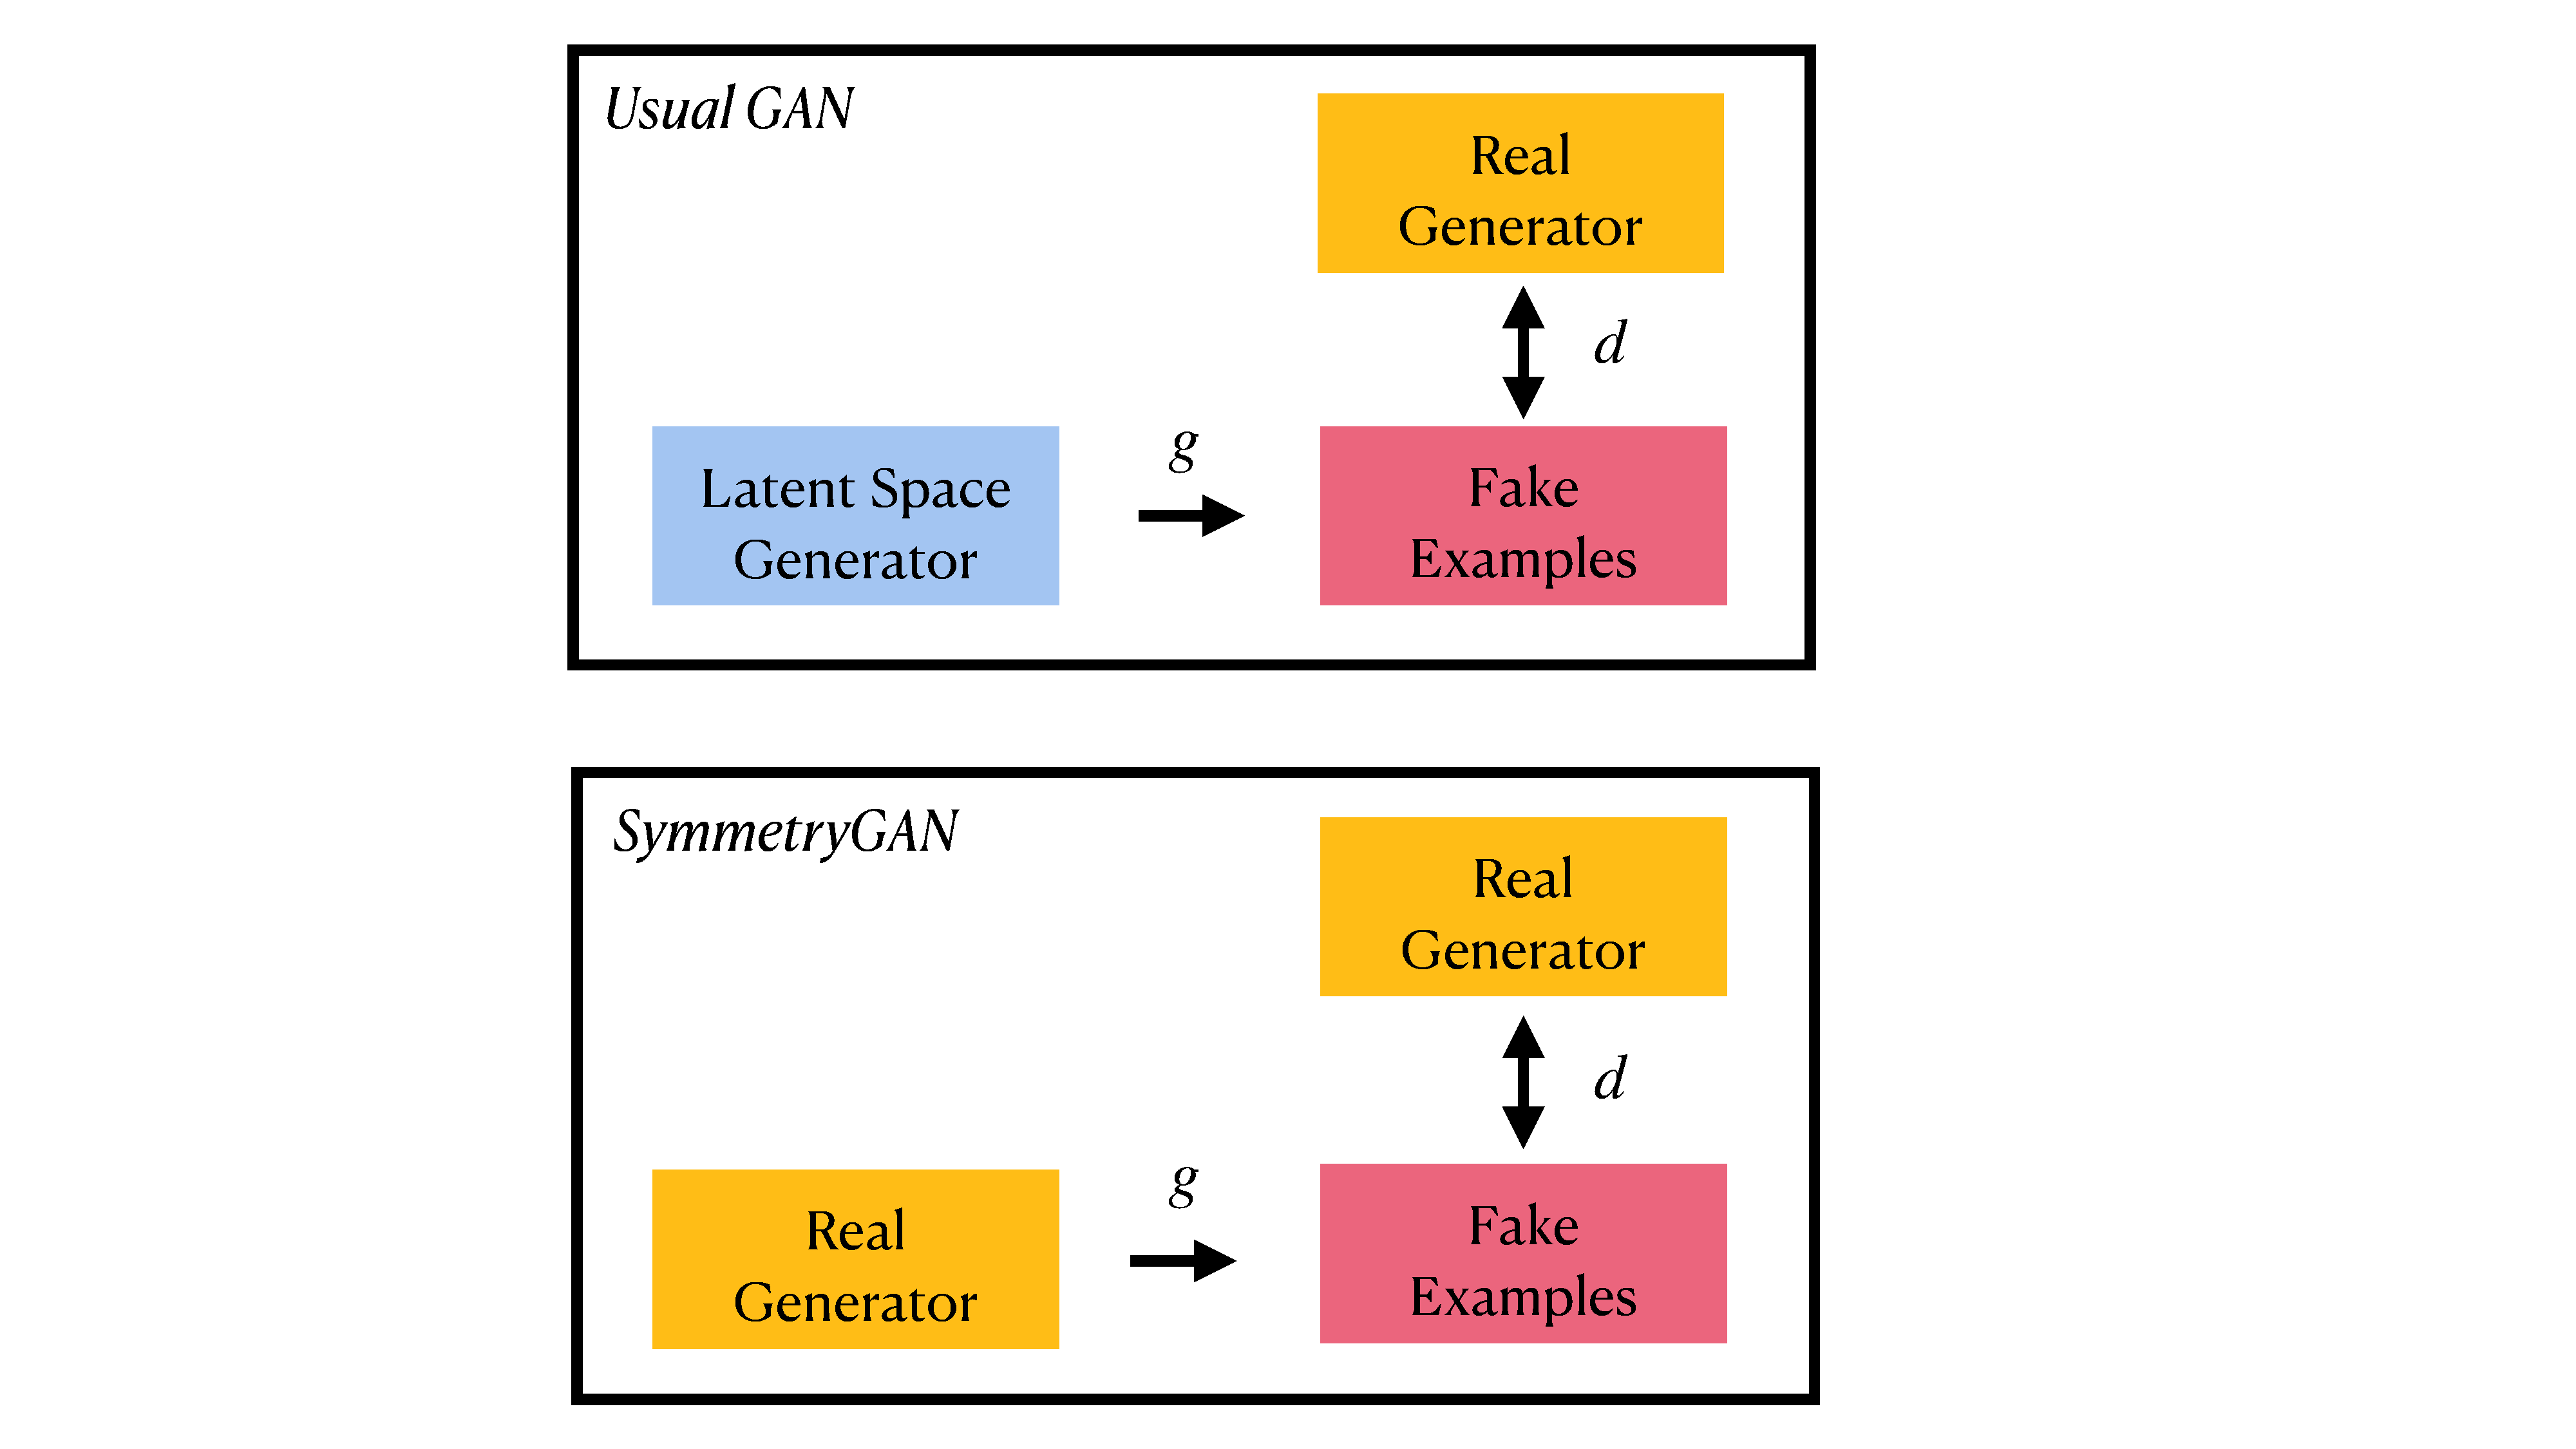
\includegraphics[width=0.6\textwidth]{figures/chapter-09/SchematicSymmetry2.pdf}
    \caption[Architectural comparison of standard GAN and SymmetryGAN for automated symmetry discovery.]{Schematic comparison of training architectures for (top) a standard Generative Adversarial Network (GAN) and (bottom) the proposed SymmetryGAN framework for automated symmetry discovery in particle physics data.
    %
    In a standard GAN, the generator $g: \mathcal{Z} \to \mathcal{X}$ maps random noise $z \sim p_z$ to synthetic data samples, while the discriminator $d: \mathcal{X} \to [0,1]$ attempts to distinguish real data $x \sim p_{\text{data}}$ from generated samples $g(z)$. The adversarial training objective drives $g$ to match the data distribution without explicit physics constraints.
    %
    The SymmetryGAN architecture modifies this framework with a symmetry transformation module $g_\theta: \mathcal{X} \to \mathcal{X}$, parametrized by learnable parameters $\theta$, which acts on both real samples. The discriminator receives transformed pairs $(x, T_\theta(x)),$ learning to identify distribution preserving transformations. When the discriminator cannot distinguish between a sample and its transformed version, the transformation $T_\theta$ represents an symmetry of the distribution.
    %
    The inertial reference dataset, while not explicitly shown in this diagram, is incorporated directly into the generator architecture in \cref{sec:empirical-experiments}}
    \label{fig:schematic}
\end{figure}
    \cref{fig:schematic} shows the modified GAN architecture of \textsc{SymmetryGAN}.
    
    \subsection{Machine Learning with Inertial Restrictions}
    The incorporation of inertial reference densities, as established in \cref{subsec:inertial_densities}, presents both theoretical necessity and practical challenges.
    %
    These restrictions can be implemented through three distinct approaches.
    \begin{enumerate}
        \item \textbf{Simultaneous discrimination}:
            %
            In this approach, discriminators evaluate transformations on both the target dataset and samples from the inertial density.
            %
            The loss function is extended to include terms from the inertial distribution \(p_I\)
            \[
                \widetile L[g,d,d_I] = L[g,d] + \lambda L_I[g,d_I]
            \]
            where \(d_I\) is a separate discriminator network specialized for the inertial distribution.
            %
            This method offers maximal flexibility, allowing discovery of symmetries even when the inertial distribution's symmetries are not known analytically.
            %
            However, it requires the ability to sample from \(p_I\) which becomes problematic for improper priors like uniform distributions on \(\mathbb{R}^n\).
        \item \textbf{Two stage selection}:
            %
            This approach involves first identifying all PDF preserving maps, then filtering for those preserving the inertial density.
            %
            The two stage approach decouples the symmetry discovery problem into training multiple generators to find PDF preserving transformations of the target data and \textit{post hoc} verifying which transformations also preserve \(p_I\)
            %
            While conceptually clean, this method proves computationally wasteful, as the space of PDF preserving maps vastly exceeds the space of true symmetries.
        \item \textbf{Upfront restriction}:
            %
            Here one constrains the generator architecture to only produce transformations that preserve the inertial density by construction in the first place, using prior knowledge about \(p_I\).
    \end{enumerate}
    
    It is this third approach that is adopted in the \textsc{SymmetryGAN} implementation.
    %
    When the inertial distribution is uniform on \(\mathbb{R}^n\) the generator should be restricted to equiareal maps---transformations with unit Jacobian determinant, as shown in \cref{eq:equiareal-maps}.
    %
    The intersection of the equiareal group and affine group \(\operatorname{Aff}_n(\R)\) corresponds to the affine special linear group \(\mathbb{A}SL^\pm_n(\mathbb{R})\) and its extensions.

    The upfront restriction method offers computational efficiency gains by searching only among valid symmetries in addition to theoretical guarantees that discovered transformations are true symmetries.
    %
    It also simplifies training without multiple discriminators or \textit{post hoc} verification.

    The restriction to affine equiareal maps, while limiting, captures a rich class of symmetries including rotations, reflections, shears, and all their compositions.
    %
\begin{theorem}[Iwasawa Decomposition of the Affine Group~\cite{iwasawa_types_1949}]
\label{thm:iwasawa_affine}
Let 
\[
    \operatorname{Aff}_n(\R)= GL_n(\R)\ltimes\R^n
\]
be the real affine group.  Define the subgroups
\[
\begin{aligned}
Z &= \{\pm I_n\}\cong \mathbb{Z}_2,\\
K &= SO(n),\\
A &= \bigl\{D(\vb r)=\operatorname{diag}(r_1,\dots,r_n)\;\big|\;r_i\in(0,\infty)\bigr\},\\
N &= \bigl\{S(u) \;\big|\;S_{ii}=1,\ S_{i < j}\in\R, S_{i>j}=0\bigr\},\\
V &= \qty{\vb v \mid v_i\in\R }\cong\R^n.
\end{aligned}
\]
Then every element $M\in\operatorname{Aff}_n(\R)$ admits a unique factorisation
\[
M \;=\;
\sqrt{|\det M|}\;\bigl(\pm I_n\bigr)^{\frac{1-\text{sgn}(\det M)}{2}}
\;R(\vb\theta)\;D(\vb r)\;S(u) + \vb v,
\]
where
\)
\pm I_n\in Z,\quad R(\vb\theta)\in K,\quad D(\vb r)\in A,\quad S(u)\in N,\quad \vb v\in V.
\)
\end{theorem}
\noindent\textbf{Example (}\(n=2\)\textbf{).}  In two dimensions these matrices take the form
\begin{gather}
I_2=\begin{bmatrix}1&0\\0&-1\end{bmatrix},\\
R(\theta)=\begin{bmatrix}\cos\theta & -\sin\theta\\
\sin\theta & \cos\theta\end{bmatrix},\\
D(r)=\begin{bmatrix}r & 0\\0 & r^{-1}\end{bmatrix},\\
S(u)=\begin{bmatrix}1 & u\\0 & 1\end{bmatrix},\\
v=\begin{bmatrix}v_1\\v_2\end{bmatrix}.
\end{gather}
Hence every $g\in\operatorname{Aff}_2(\R)$ admits the six parameter representation
\[
g(x)=\sqrt{|d|}\,\bigl(I_2\bigr)^{\frac{1-\sgn(d)}{2}}
R(\theta)\,D(r)\,S(u)\,x \;+\;v,
\qquad d=\det g,
\]
which is well suited to gradient based optimization over the space of affine symmetries.

\subsection{Deep learning implementation details.}

    The practical implementation of \textsc{SymmetryGAN} requires careful attention to architectural choices, training dynamics, and numerical stability.
    %
    The framework's success depends on balancing the adversarial training process while maintaining the theoretical properties that enable symmetry discovery.
    
    For linear symmetries, the generator directly parametrises transformation matrices.
    %
    Rather than using fully connected layers, the generator outputs parameters of the Iwasawa decomposition, ensuring all generated transformations lie within the constrained search space.
    %
    This architectural choice provides interpretability, where each parameter has clear geometric meaning, stability, by avoiding ill conditioned matrices through structured parametrisation, and efficiency, by reducing the parameter count compared to unconstrained matrices from \(n^2\) to \(\nicefrac{n(n-1)}{2}.\)

    To investigate specific symmetry subgroups, the loss function can further incorporate additional constraints.
    %
    For example, to find cyclic symmetries \(\mathbb{Z}_q\) the loss can be augmented to encourage \(g^q = \mathbbm{1}\).
    \[
        \label{eq:cyclic-loss}
        L_{\text{cyclic}}[g,d] = L_{\text{BCE}}[g,d] + \alpha \sum_{i} ||g^q(x_i) - x_i||^2.
    \]

    The discriminator architecture should follow standard practices for the data domain.
    %
    For low dimensional examples, simple feedforward networks with \(2-3\) hidden layers suffice.

    Analysing the loss landscape reveals its topological structure.
    %
    For simple distributions like Gaussians, the loss landscape contains distinct maxima corresponding to each symmetry, separated by deep valleys.
    %
    This topology explains why random initialisation reliably discovers different symmetries.
    %
    The generator converges to the nearest local maximum, which corresponds to a true symmetry, and there is no reason to expect that the nearest local maximum for any given random initialisation should be the identity map.

    The framework demonstrates remarkable robustness to hyperparameter choices.
    %
    Across experiments with Gaussian mixtures and particle physics data, a range of hyperparameter settings achieve consistent symmetry discovery.

    \subsection{Verification.}
    A few different checks can be applied to verify that the discovered transformation represents a true symmetry.
    \begin{itemize}
        \item \textbf{Visual inspection}: Visually inspecting low dimensional slices of the original and transformed data serves as a simple sniff test.
        \item \textbf{Loss value}: True symmetries always achieve a loss of \(2\log2\) at convergence. Hence measuring the loss function at discovered transformations can validate whether the transformation is a symmetry or not.
        \item \textbf{Distribution matching}: Statistical divergences between \(X\) and \(g(X)\) such as the KL divergence measure whether the two datasets have the same probability density or not.
        \item Invariant verification: known invariants, such as moments, should be identical between the distributions.
    \end{itemize}
    
    \subsection{Other symmetry discovery methods.}
        The landscape of symmetry discovery in machine learning has evolved considerably, with approaches ranging from classical statistical methods to modern deep learning architectures.
        %
        Understanding \textsc{SymmetryGAN}'s position within this ecosystem illuminates both its unique contributions and its connections to broader methodological trends.

        Classical statistical approaches traditionally rely on hypothesis testing and moment matching.
        %
        These methods typically test specific, predefined symmetry hypotheses by relying on low dimensional projections or summary statistics.
        %
        They struggle with high dimensional data or complex symmetry groups and require extensive domain knowledge to formulate appropriate tests.

        The Cramer-von Mises~\cite{von_mises_wahrscheinlichkeit_1928, cramer_composition_1928} and Anderson-Darling tests~\cite{anderson_asymptotic_1952} exemplify this approach to check whether transformed data follows the same distribution as the original.
        %
        While rigorous, these methods scale poorly and cannot discover unexpected symmetries, they can only validate known symmetries.

        Machine learning methods introduced automation to the symmetry discovery process.
        %
        Methods like Group-Invariant Autoencoders~\cite{Hao2023LorentzAutoencoders} learn representations invariant to known symmetry groups but cannot discover unknown symmetries
        %
        Spatial Transformer Networks~\cite{Jaderberg2015SpatialNetworks} learn task-specific transformations but don't explicitly identify symmetries \textit{per se}.
        %
        Maximum Mean Discrepancy approaches~\cite{tolstikhin_minimax_2016} and other kernel methods can test symmetry but struggle with continuous groups.

        Contemporary deep learning methods have introduced a range of innovations to the field.
        %
        Lie Group Learning Networks directly parametrise Lie algebra generators~\cite{gabel_learning_2023}.
        %
        Such methods have excellent theoretical grounding, and physically interpretable parameters.
        %
        They are, however, restricted to continuous symmetries, and require complex optimisation for convergence.
        %
        Latent LieGAN (LaLiGAN) enables the discovery nonlinear symmetries via latent space linearization~\cite{yang_latent_2024}.
        %
        It made strides in handling non-linear group actions, but the additional complexity leads to potential latent space artifacts

        \textsc{SymmetryGAN} exemplifies several important trends in modern machine learning for HEP.
        %
        Methods have broadly benefited from incorporating domain knowledge through architectural constraints and loss terms.
        %
        In general the rise of equivariant learning has driven the move beyond invariance to discover the underlying symmetry structure.
        
        \textsc{SymmetryGAN} also exemplies the trend towards interpretability by producing human understandable symmetry parameters rather than opaque features.
        %
        The method is however limited in its restriction to parametrisable symmetry classes.
        %
        It also exclusively enables symmetry discovery, the task of identifying elements of the symmetry group of a dataset.
        %
        Although the work does provide some steps towards symmetry inference, the task of identifying and classifying the symmetry group as a whole, it remains challenging to infer complete symmetry group structure from discovered elements.
        
        The field continues to evolve rapidly, with \textsc{SymmetryGAN} representing a significant step toward automated, theoretically grounded symmetry discovery.
        %
        Its success in particle physics applications, detailed in the following section, demonstrates the practical value of this principled approach to uncovering hidden invariances in complex data.

\section{Empirical experiments.}
\label{sec:empirical-experiments}
        The theoretical machinery of \textsc{SymmetryGAN}, with its rigorous statistical framework and inertial reference densities, proves its worth through empirical validation.
        %
        Moving from abstract formulations to concrete applications reveals both the method's effectiveness and challenges that might drive future research.
        %
        This section details the application of this method on carefully controlled Gaussian experiments to complex collider data, demonstrating how \textsc{SymmetryGAN} bridges the gap between mathematical elegance and practical discovery.

        \subsection{Gaussian experiments.}
            The choice to begin with Gaussian distributions reflects more than mere mathematical convenience; it represents a strategic approach to validating a novel methodology.
            %
            Gaussians offer analytically tractable loss landscapes that allow direct comparison between theoretical predictions and empirical results, serving as a crucial proof of concept before tackling high dimensional HEP data.

            \subsubsection{One-dimensional Gaussian.}
                The simplest non-trivial test case consists of a Gaussian distribution \(\mathcal{N}(0.5,1.0)\) with a reflection symmetry about \(x=0.5\).
                %
                This apparently simple example harbours surprising richness.
                %
                The disconnected nature of the symmetry space in even this simple example demonstrates the training dynamics in a \textsc{SymmetryGAN.}

                The distribution admits precisely two linear symmetries: the identity transformation \(g(x)=x\) and the reflection \(g(x)=1-x\).
                %
                When the generator is parametrised as an arbitrary one dimensional affine transformation, \(g(x)=b+cx\), the analytic loss landscape has the topology shown in \cref{fig:Z2analytic}.
                %
                The two maxima corresponding to these symmetries are separated by a deep valley at \(c=0\), creating a disconnected solution space.
 \begin{figure}
     \centering
     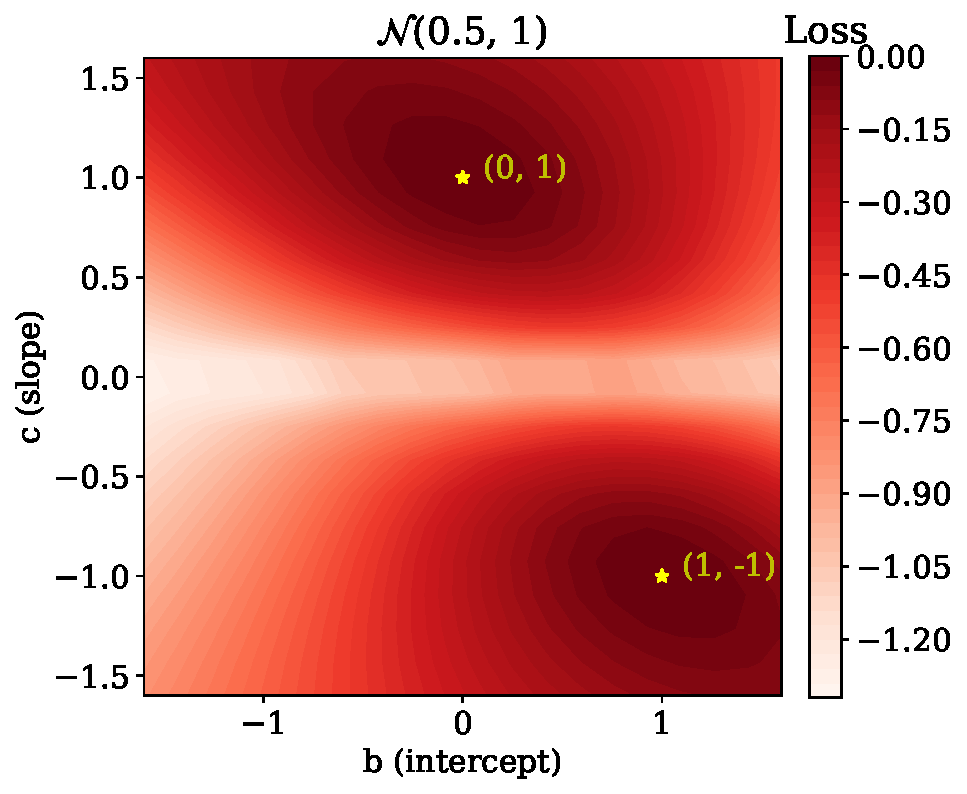
\includegraphics[width=0.6\linewidth]{figures/chapter-09/Z2analytic.pdf}
     \caption{Analytic loss landscape for the one-dimensional uniform distribution $\mathcal{N}((0.5,1))$ under affine transformations $g(x) = b + cx$. The landscape exhibits two distinct maxima (indicated by stars) corresponding to the identity transformation $(b,c) = (0,1)$ and reflection $(b,c) = (1,-1)$, separated by a deep valley at $c = 0$.
     %
     This topological barrier creates a disconnected solution space that deterministically routes optimisation trajectories based on initial parameter values.
     }
     \label{fig:Z2analytic}
 \end{figure}               
                The empirical results validate the theoretical predictions with remarkable precision.
                %
                Random initialisation of parameters \((b_i, c_i) \sim \mathcal{U}([-5, 5]^2)\) leads to convergence at one of two distinct clusters: \((b_f, c_f) = (0, 1)\) for the identity or \((1, -1)\) for the reflection as can be seen in \cref{fig:Z2numeric}.
                %
                The loss barrier at \(c=0\) acts as a watershed, deterministically routing the optimisation based on the sign of the initial slope.
                %
                This behaviour illuminates that the loss landscape topology directly determines the discoverable symmetry structure.
\begin{figure}
    \centering
    \begin{subfigure}[b]{0.31\textwidth}
        \centering
        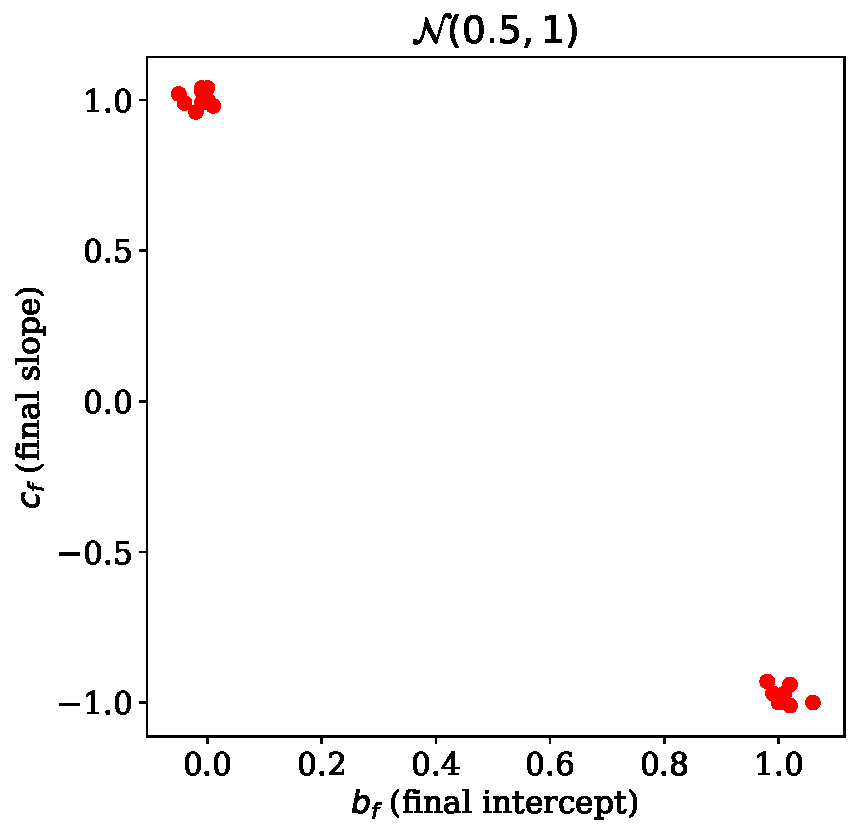
\includegraphics[width=\textwidth]{figures/chapter-09/b_fc_f.pdf}
        \caption{}
        \label{fig:Z2numeric_i}
    \end{subfigure}
    \hfill
    \begin{subfigure}[b]{0.31\textwidth}
        \centering
        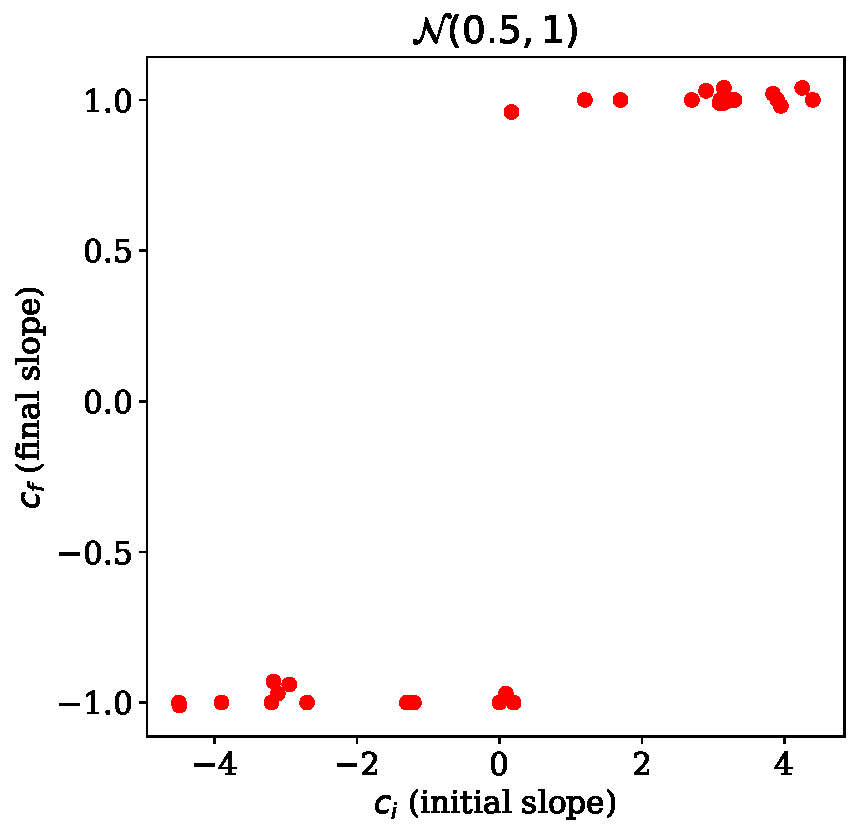
\includegraphics[width=\textwidth]{figures/chapter-09/c_ic_f.pdf}
        \caption{}
        \label{fig:Z2numeric_ii}
    \end{subfigure}
    \hfill
    \begin{subfigure}[b]{0.31\textwidth}
        \centering
        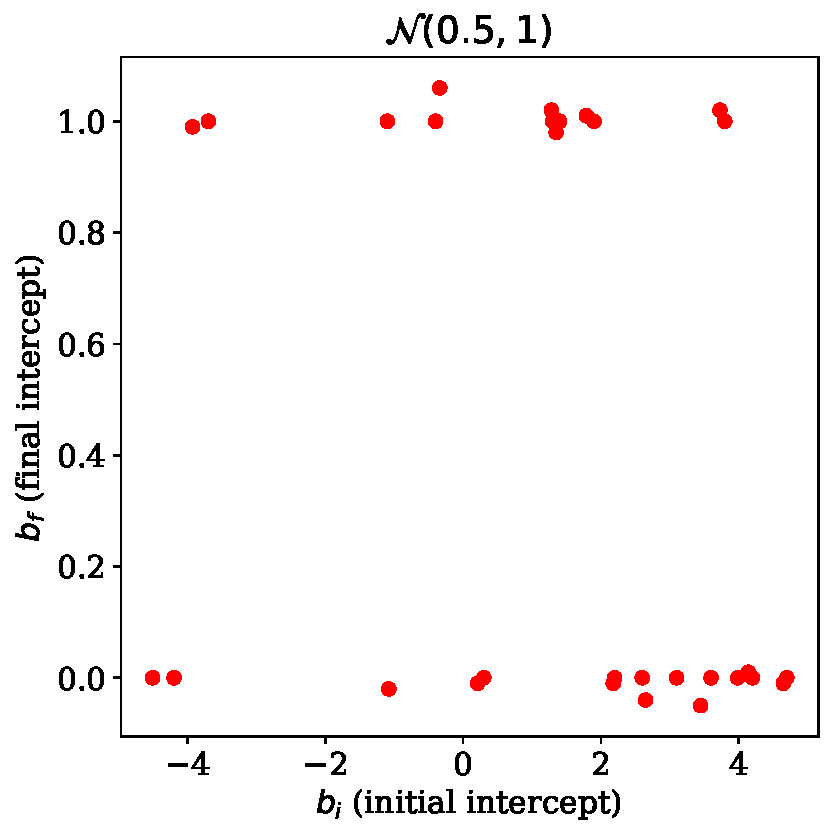
\includegraphics[width=\textwidth]{figures/chapter-09/b_ib_f.pdf}
        \caption{}
        \label{fig:Z2numeric_iii}
    \end{subfigure}
    \caption[Empirical validation of \textsc{SymmetryGAN} on 1 dimensional Gaussian data showing convergence to discrete symmetries based on initial conditions.]{Empirical validation of \textsc{SymmetryGAN} on 1 dimensional Gaussian data showing convergence to discrete symmetries based on initial conditions.
    %
    Random initialisation with $(b_i, c_i) \sim \mathcal{U}([-5, 5]^2)$ leads to convergence at two distinct fixed points. (a) Distribution of final parameters $(b_f, c_f)$ reveals two clusters at $(0,1)$ and $(1,-1)$, corresponding to the identity and reflection symmetries respectively. (b) Deterministic routing based on initial slope: $c_i > 0$ converges to identity $(c_f = 1)$ while $c_i < 0$ converges to reflection $(c_f = -1)$, with a sharp phase transition at $c_i = 0$. (c) Final intercept $b_f$ shows no correlation with initial value $b_i$, demonstrating that the loss landscape has no barrier in intercept space.}
    \label{fig:Z2numeric}
\end{figure}
            \subsubsection{Two dimensional Gaussians.}
                Two dimensional Gaussian examples increase the complexity while maintaining analytical tractability.
                %
                Consider first the standard bivariate normal \(N_{1, 1} = \mathcal{N}(\mathbf{0}, \mathbbm{1}_2)\), which possesses the full orthogonal group \(O(2)\) as its symmetry group.
                %
                When the generator is restricted to the form
{\setlength{\arraycolsep}{12pt}
\[
  \label{eq:SO2_generator}
  g(x)=\begin{bmatrix}
     c & s\\
    -s & c
  \end{bmatrix}x
\]
}
                \textsc{SymmetryGAN} would be expected to discover that only transformations satisfying \(c^2 + s^2 = 1\) represent true symmetries.
                %
                As can be seen in \cref{fig:SO2-i}, the empirical results demonstrate the method's ability to learn this constraint without explicit enforcement.
                %
                Starting from random initialisations within \([-1, 1]^2\), the learned parameters consistently converge to the unit circle, validating that \textsc{SymmetryGAN} can discover not just discrete symmetries but continuous symmetry manifolds.
                %
                This represents a significant achievement: the neural network learns the algebraic constraint defining \(SO(2)\) purely from data.
\begin{figure}
    \centering
    \begin{subfigure}[b]{0.45\textwidth}
        \centering
        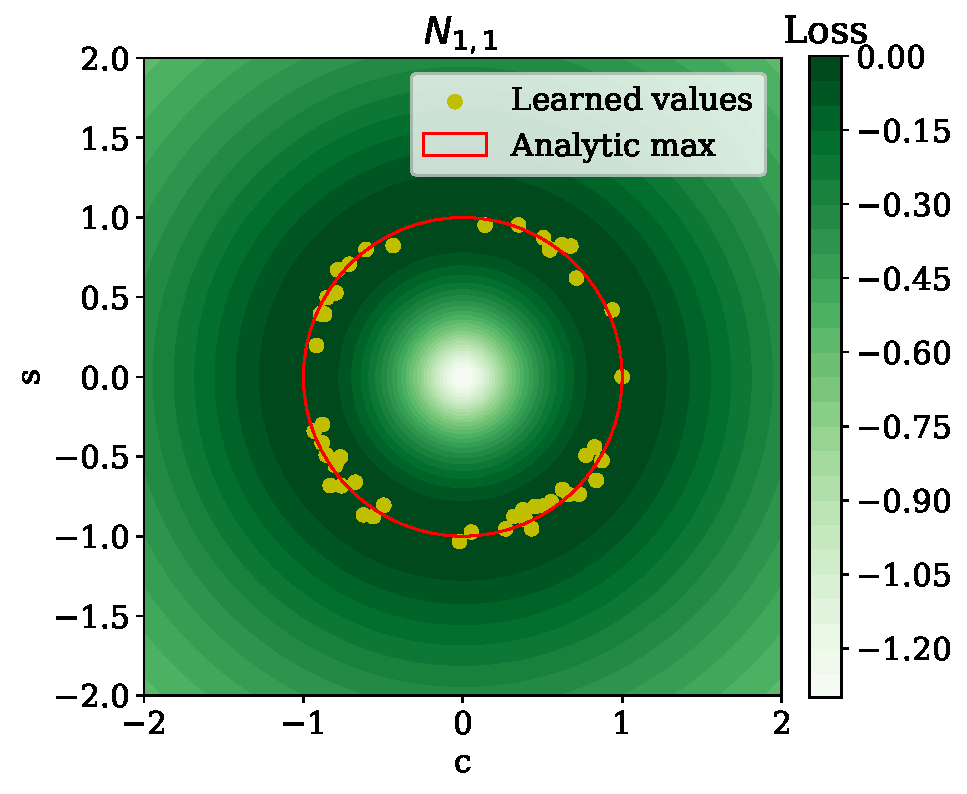
\includegraphics[width=\textwidth]{figures/chapter-09/SO2symmAnalytic.pdf}
        \caption{}
        \label{fig:SO2-i}
    \end{subfigure}
    \hfill
    \begin{subfigure}[b]{0.45\textwidth}
        \centering
        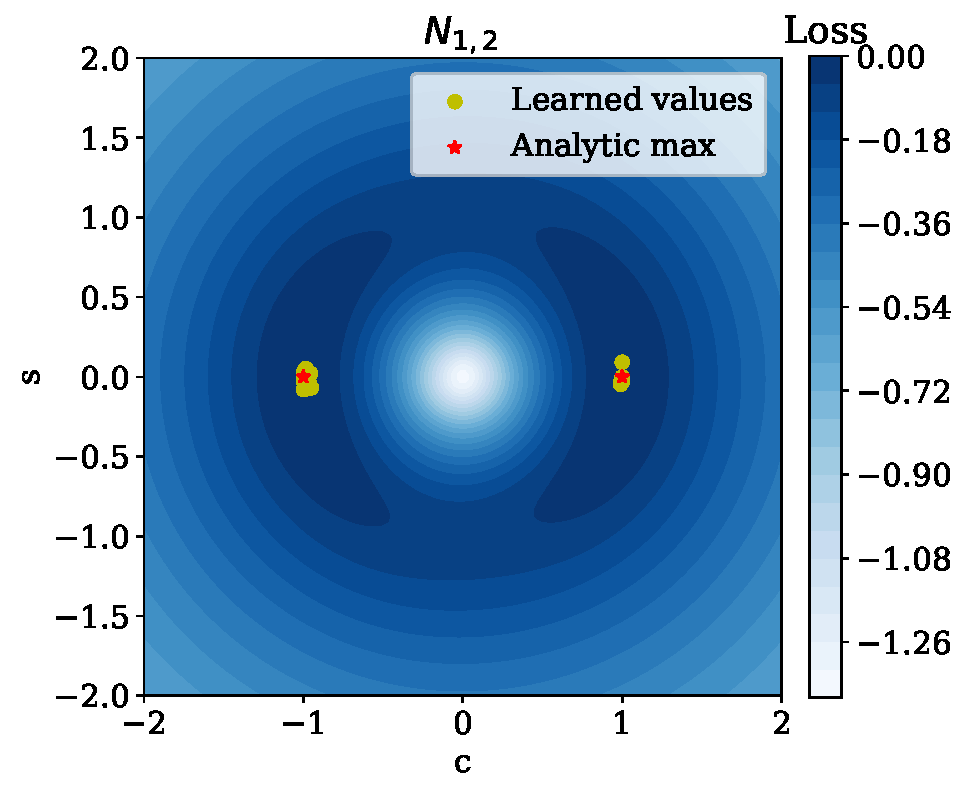
\includegraphics[width=\textwidth]{figures/chapter-09/4O2asymmAnalytic.pdf}
        \caption{}
        \label{fig:SO2-iii}
    \end{subfigure}
    \caption[Loss landscapes demonstrating \textsc{SymmetryGAN's} ability to discover continuous $SO(2)$ and discrete $V_4$ symmetries in isotropic and anisotropic 2D Gaussians.]{Analytic loss landscapes for two dimensional Gaussian distributions under rotation like transformations $g(\mathbf{x}) = \begin{pmatrix} c & -s \\ s & c \end{pmatrix}\mathbf{x}$, with empirically discovered symmetries overlaid as scatter points. (a) Isotropic Gaussian $\mathcal{N}(\mathbf{0}, \mathbbm{1})$ exhibits continuous $SO(2)$ symmetry, with loss maxima forming a circle at $c^2 + s^2 = 1$. The discovered symmetries densely populate this manifold, confirming the theoretical prediction. (b) Anisotropic Gaussian $\mathcal{N}(\mathbf{0}, \text{diag}(1,2))$ possesses only discrete Klein four--group symmetries $V_4$, with isolated maxima at $(c,s) \in \{(\pm 1, 0), (0, \pm 1)\}$. The symmetry breaking from continuous to discrete group structure is induced by the non-uniform covariance. Darker regions indicate higher loss values; stars mark theoretical optima.}
    \label{fig:SO2}
\end{figure}
\begin{figure}
    \centering
    \begin{subfigure}[b]{0.31\textwidth}
        \centering
        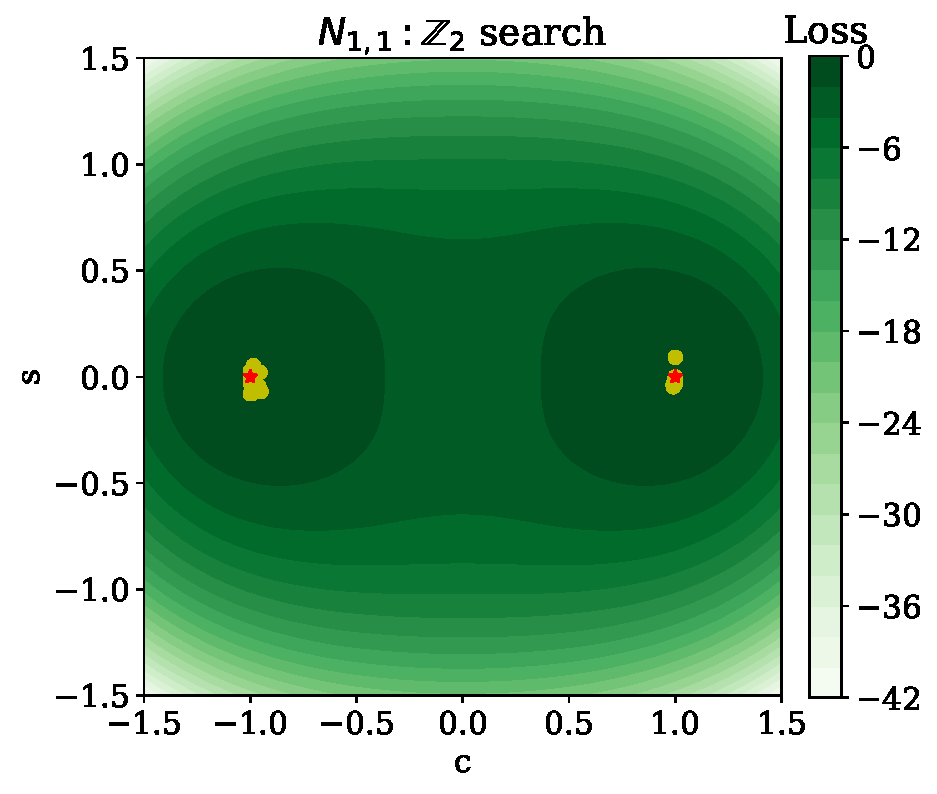
\includegraphics[width=\textwidth]{figures/chapter-09/C2MSE.pdf}
        \caption{}
        \label{fig:MSE_i}
    \end{subfigure}
    \hfill
    \begin{subfigure}[b]{0.31\textwidth}
        \centering
        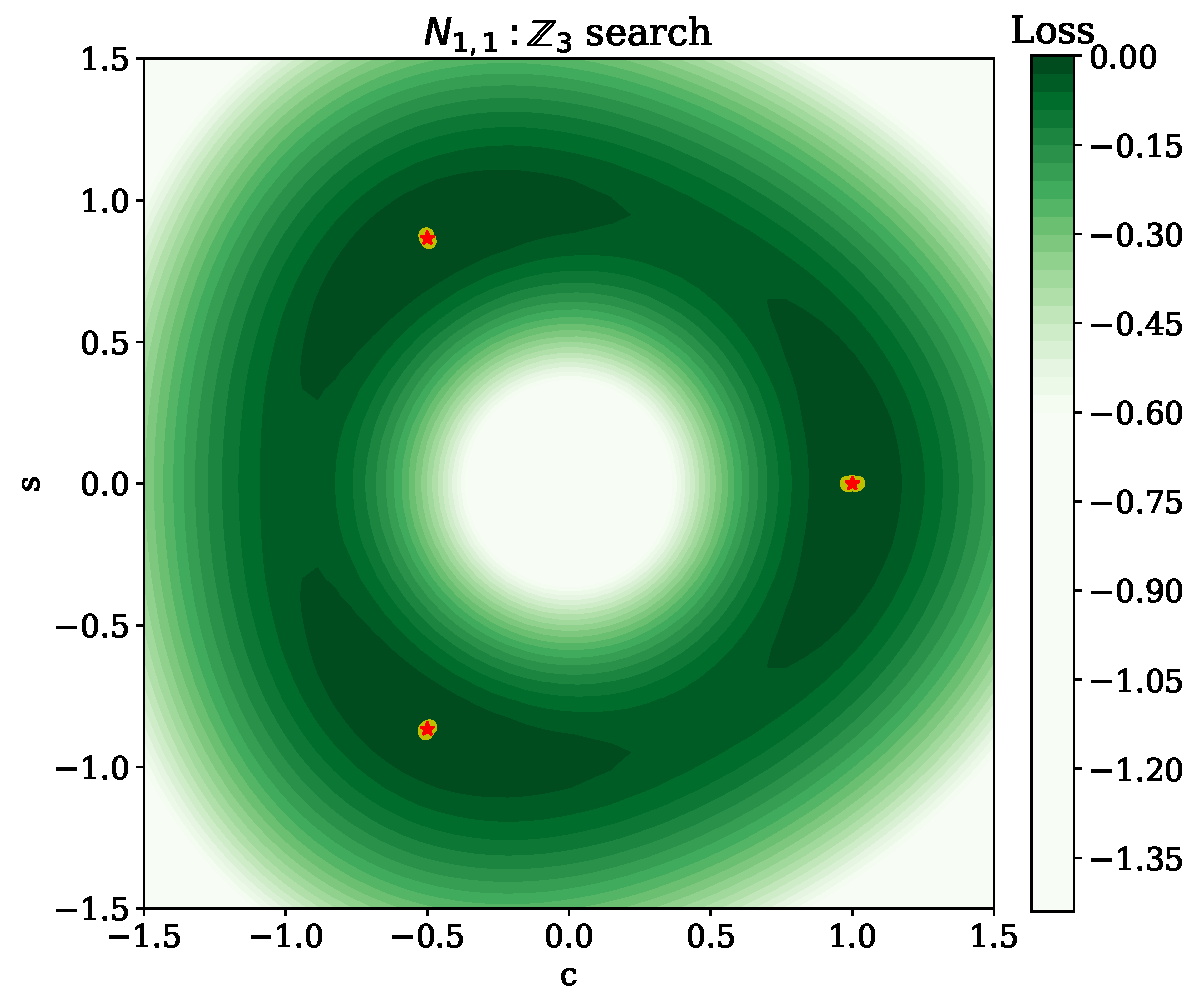
\includegraphics[width=\textwidth]{figures/chapter-09/C3MSE.pdf}
        \caption{}
        \label{fig:MSE_ii}
    \end{subfigure}
    \hfill
    \begin{subfigure}[b]{0.31\textwidth}
        \centering
        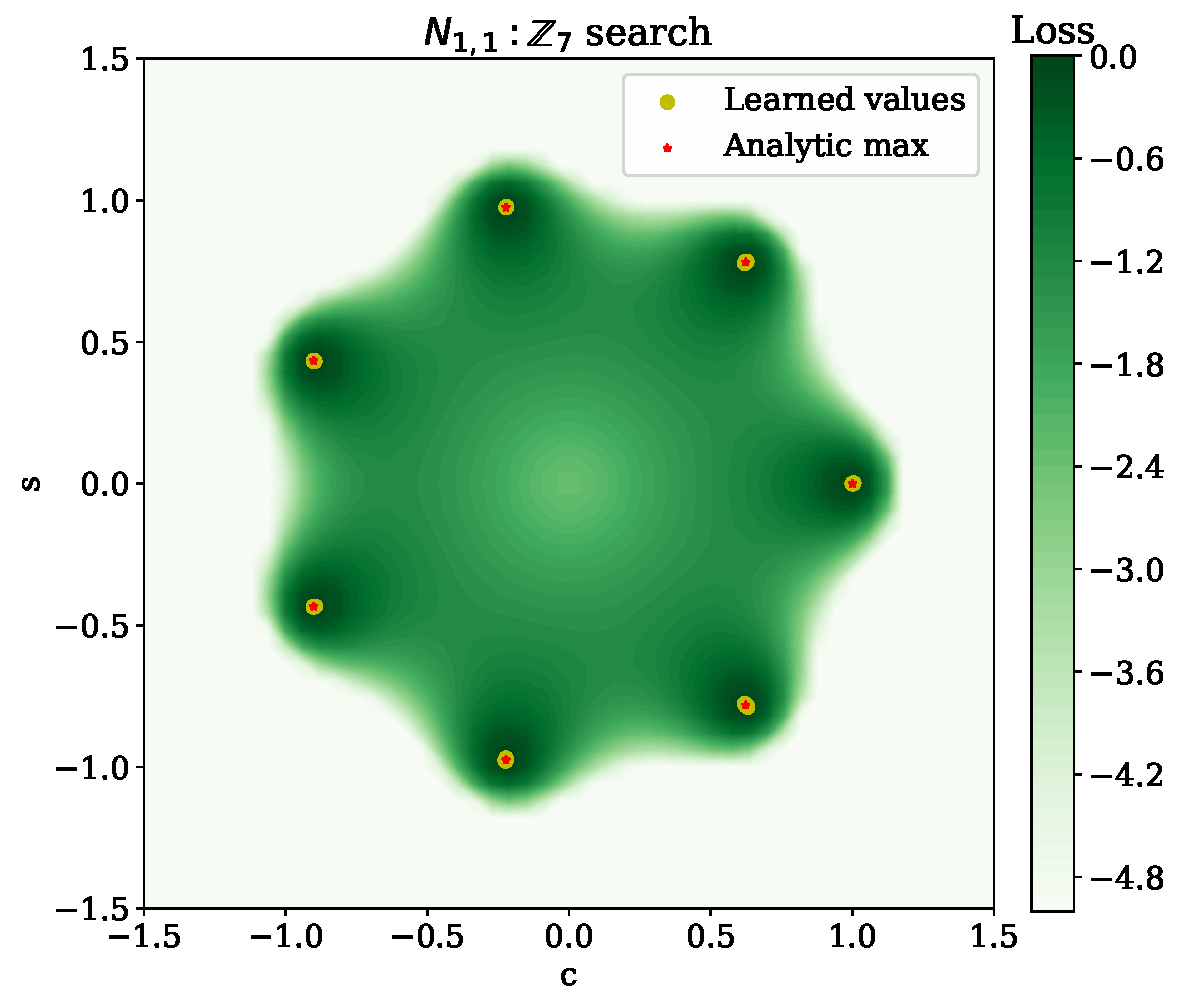
\includegraphics[width=\textwidth]{figures/chapter-09/C7MSE.pdf}
        \caption{}
        \label{fig:MSE_iii}
    \end{subfigure}
    \caption[Controlled discretization of continuous $SO(2)$ symmetry into cyclic subgroups $\mathbb{Z}_q$ via constraint enforcement.]{Controlled symmetry breaking in the isotropic Gaussian $\mathcal{N}(\mathbf{0}, \mathbbm{1})$ through cyclic constraint enforcement. The loss function is augmented with a mean squared error term $\alpha \|g^q(\mathbf{x}) - \mathbf{x}\|^2$ that enforces $q-$fold cyclic symmetry. The continuous $SO(2)$ symmetry observed in \cref{fig:SO2-i} is discretised into cyclic subgroups: (a) $\mathbb{Z}_2$ symmetry with $q=2$, showing two antipodal maxima at $(c,s) = (\pm 1, 0)$; (b) $\mathbb{Z}_3$ symmetry with $q=3$, displaying three maxima at the cube roots of unity; (c) $\mathbb{Z}_7$ symmetry with $q=7$, exhibiting seven equally spaced maxima on the unit circle. The discovered symmetries (scatter points) precisely align with the $q^{\text{th}}$ roots of unity, validating the theoretical prediction that the cyclic constraint induces symmetry discovery of discrete components. Darker regions indicate higher loss values, stars indicate analytic maxima.}
    \label{fig:MSE}
\end{figure}               

                The two dimensional Gaussian example also allows us to test the approach described in \cref{eq:cyclic-loss}.
                %
                \cref{fig:MSE} shows the discovered symmetries for the \(N_{1, 1}\) distribution when the loss function is augmented with the constraint \cref{eq:cyclic-loss}, for \(q = 2, 3,\) and \(7\), with \(\alpha = 0.1\).
                %
                Both the analytic loss landscape and \textsc{SymmetryGAN}'s output confirm that the continuous \(SO(2)\) symmetry is split into discrete symmetries at the \(q^{th}\) roots of unity upon the inclusion of the mean squared error term.

                One could also consider a two dimensional Gaussian with a non-trivial covariance matrix, such as \(N_{1, 2} = \mathcal{N}(\mathbf{0}, \text{diag}(1, 2)\).
                %
                The full symmetry group of this distribution is highly non-trivial and is described below, but among other features, it contains as a subgroup the Klein \(4-\)group \(V_4 = \qty{\mathbbm{1}, -\mathbbm{1}, \sigma_3, -\sigma_3}\) for the Pauli matrix \(\sigma_3\).
                %
                When \textsc{SymmetryGAN} is limited to transformations of the form \cref{eq:SO2_generator}, it discovers the Klein \(4-\)group \(V_4\) as demonstrated in \cref{fig:SO2-iii}.
                %
                When the generator is allowed to search for general linear transformations inside \(\operatorname{Aff}_2(\mathbb{R})\), it discovers the full symmetry group that comprises the aforementioned Klein \(4-\)group as well as transformations involving dilatations.

                \cref{fig:AGL2symm} shows the discovered symmetries for the \(N_{1, 1}\) distribution and \cref{fig:AGL2asymm} shows the discovered symmetries for \(N_{1, 2}\) when the generator is able to discover general affine transformations in \(\operatorname{Aff}_2(\R).\)
\begin{figure}
    \centering
    \begin{subfigure}[b]{0.31\textwidth}
        \centering
        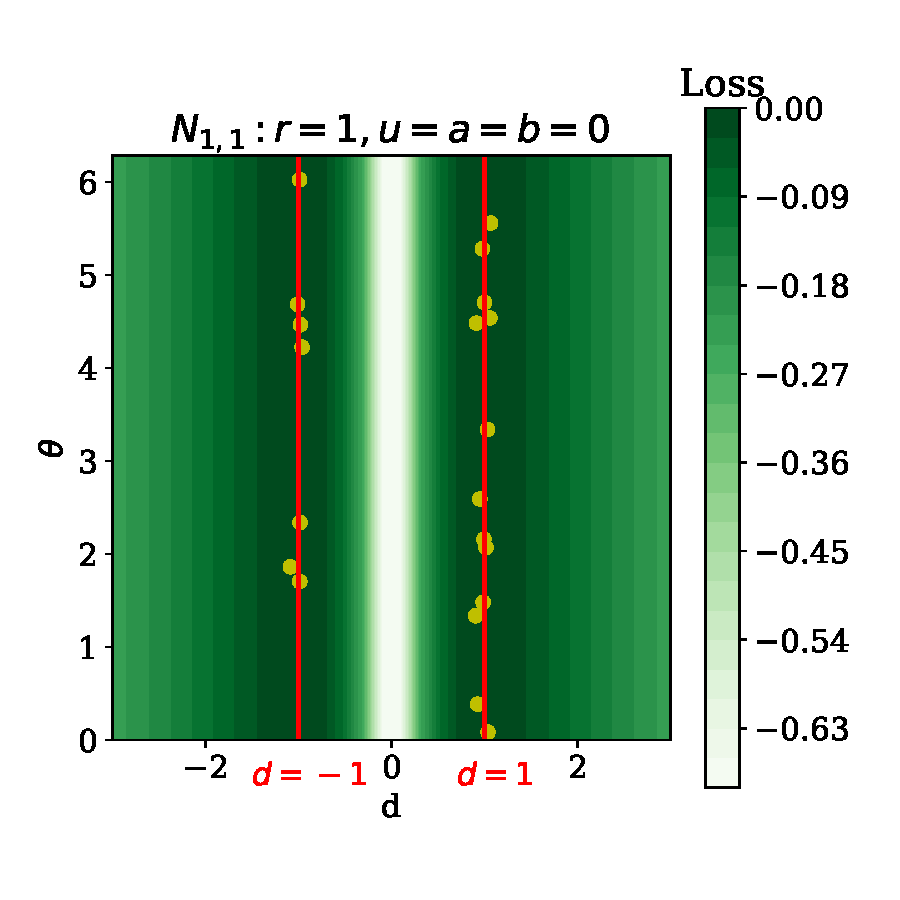
\includegraphics[width=\textwidth]{figures/chapter-09/6O2d-tsymm.pdf}
        \caption{}
        \label{fig:AGL2symm_i}
    \end{subfigure}
    \hfill
    \begin{subfigure}[b]{0.31\textwidth}
        \centering
        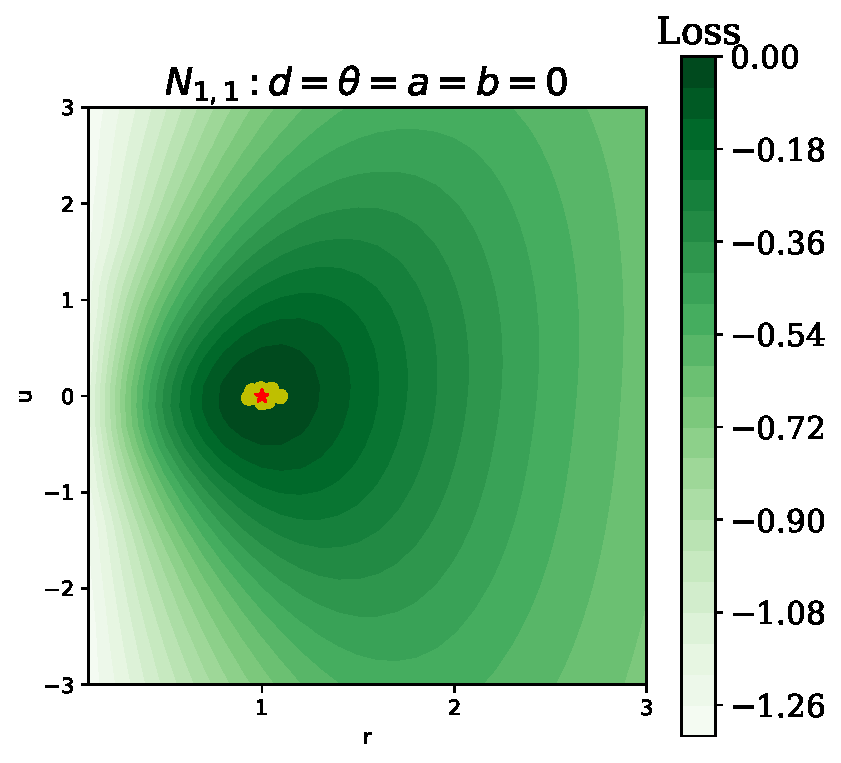
\includegraphics[width=\textwidth]{figures/chapter-09/6GL2symmRU.pdf}
        \caption{}
        \label{fig:AGL2symm_ii}
    \end{subfigure}
    \hfill
    \begin{subfigure}[b]{0.31\textwidth}
        \centering
        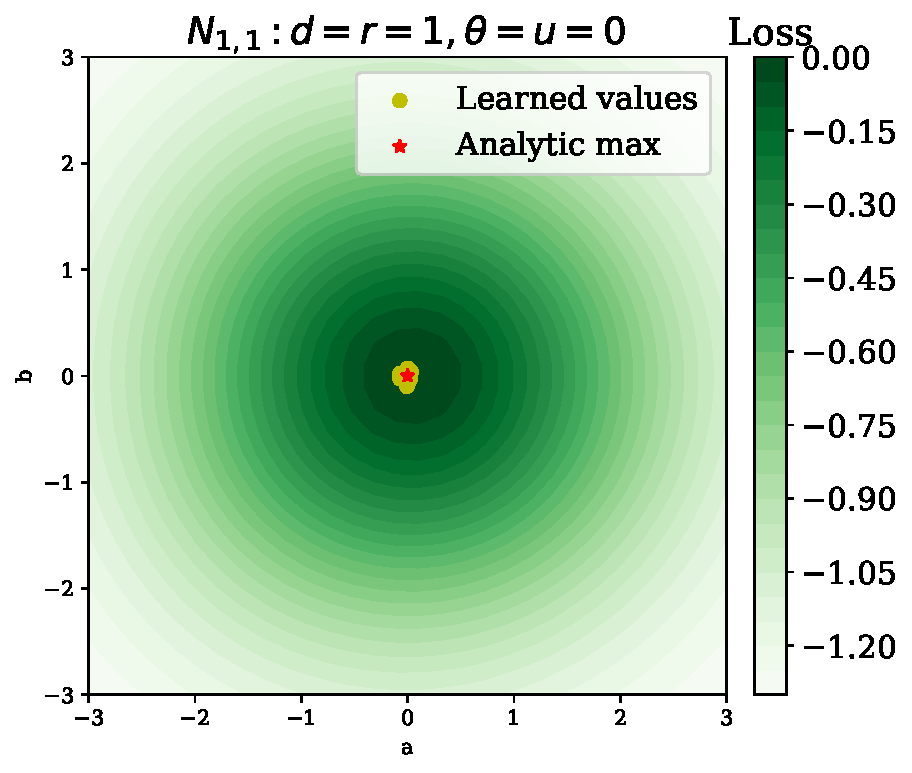
\includegraphics[width=\textwidth]{figures/chapter-09/6GL2symmAB.pdf}
        \caption{}
        \label{fig:AGL2symm_iii}
    \end{subfigure}
    \caption[Orthogonal slices of $\operatorname{Aff}_2(\mathbb{R})$ symmetries for isotropic Gaussian.]{Symmetry discovery in the full affine group $\operatorname{Aff}_2(\mathbb{R})$ for the isotropic Gaussian $\mathcal{N}(\mathbf{0}, \mathbbm{1})$, decomposed via Iwasawa parametrization $g = \sqrt{|d|} I^{\frac{1-\text{sgn}(d)}{2}} \cdot R(\theta) \cdot D(r) \cdot S(u) + \mathbf{v}$. Three orthogonal slices through the 6 dimensional loss landscape reveal the symmetry structure: (a) Determinant-rotation space $(d, \theta)$ shows continuous maxima along $d = \pm 1$ (vertical red lines) for all rotation angles. (b) Dilation-shear space $(r, u)$ exhibits a unique maximum at $(r, u) = (1, 0)$ (red star), indicating that only uniform scaling preserves the isotropic structure. (c) Translation space $(v_1, v_2)$ peaks at the origin (red star), verifying that the centred Gaussian admits no translational symmetries. Empirically discovered transformations (yellow points) cluster precisely at the theoretical optima, validating the analytic predictions.}
    \label{fig:AGL2symm}
\end{figure}
\begin{figure}
    \centering
    \begin{subfigure}[b]{0.31\textwidth}
        \centering
        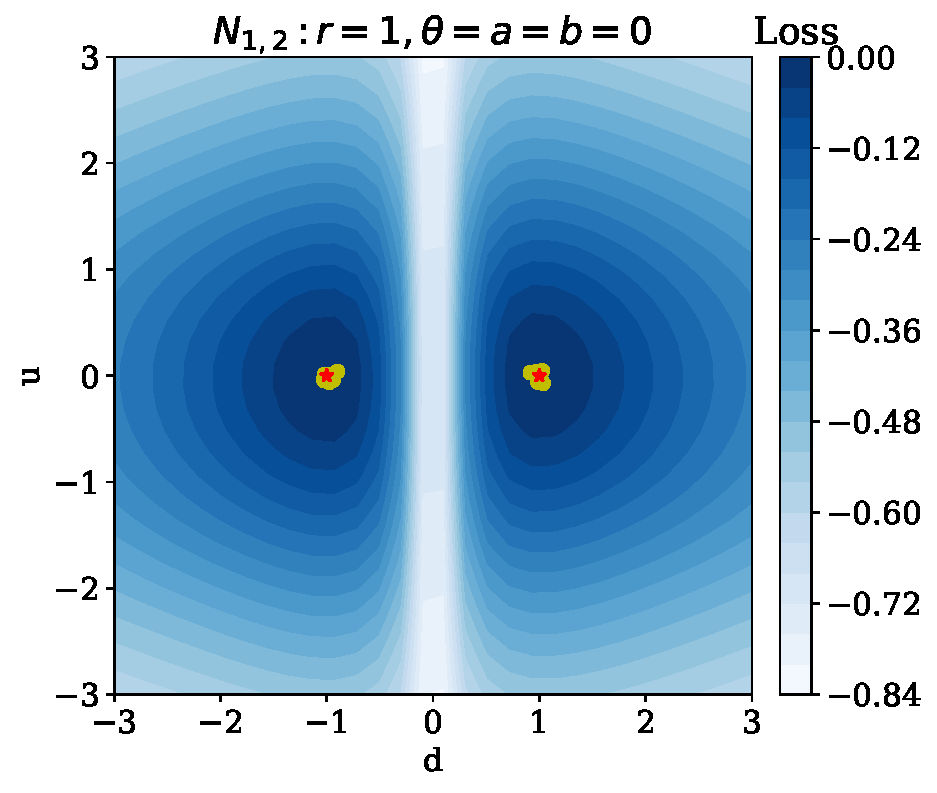
\includegraphics[width=\textwidth]{figures/chapter-09/6GL2asymmDU.pdf}
        \caption{}
        \label{fig:AGL2asymm_i}
    \end{subfigure}
    \hfill
    \begin{subfigure}[b]{0.31\textwidth}
        \centering
        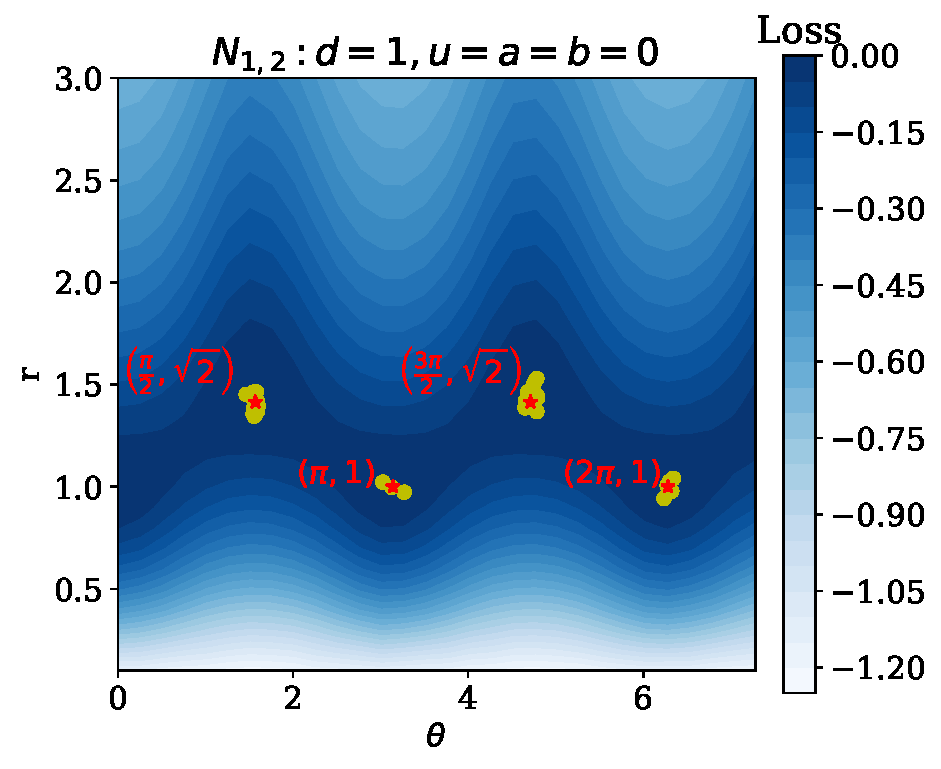
\includegraphics[width=\textwidth]{figures/chapter-09/6GL2asymmTR.pdf}
        \caption{}
        \label{fig:AGL2asymm_ii}
    \end{subfigure}
    \hfill
    \begin{subfigure}[b]{0.31\textwidth}
        \centering
        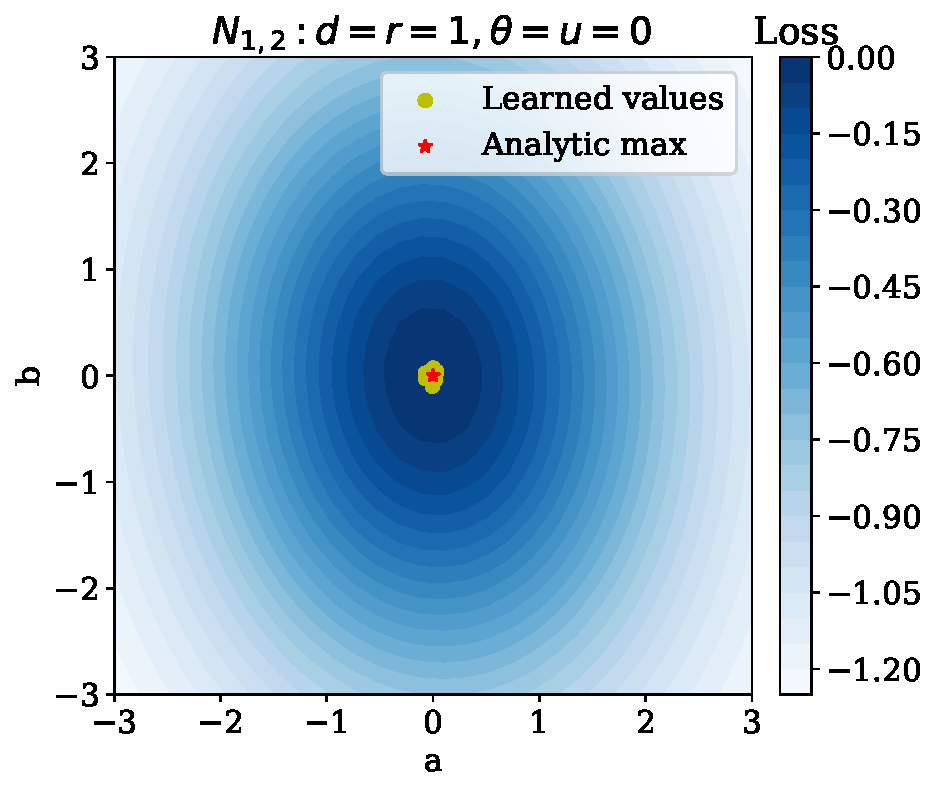
\includegraphics[width=\textwidth]{figures/chapter-09/6GL2asymmAB.pdf}
        \caption{}
        \label{fig:AGL2asymm_iii}
    \end{subfigure}
    \caption[Discrete symmetry structure of anisotropic Gaussian in $\text{Aff}_2(\mathbb{R})$ discovered by \textsc{SymmetryGAN}.]{Symmetry discovery in $\text{Aff}_2(\mathbb{R})$ for the anisotropic Gaussian $\mathcal{N}(\mathbf{0}, \text{diag}(1,2))$, revealing discrete symmetry breaking compared to the isotropic case (\cref{fig:AGL2symm}). The anisotropic covariance structure constrains the symmetry group to a supergroup of the Klein four-group $V_4$: (a) Determinant-shear space $(d, u)$ exhibits two isolated maxima (red stars) at $(d, u) \in \{(1, 0), (-1, 0)\}$, corresponding to orientation-preserving and orientation-reversing transformations with no shear. (b) Dilation-rotation space $(r, \theta)$ shows four discrete maxima (red stars) at $(r, \theta) \in \{(1, 0), (1, \pi), (\sqrt{2}, \pi/2), (\sqrt{2}, 3\pi/2)\}$, representing identity, $\pi$-rotation, and the two coordinate flips scaled by $\sqrt{2}$ to account for the eigenvalue ratio. (c) Translation space $(v_1, v_2)$ remains peaked at the origin (red star), confirming no translational symmetries. The discovered transformations (yellow points) cluster at these discrete locations, demonstrating how anisotropy breaks continuous symmetries into a discrete group.}
    \label{fig:AGL2asymm}
\end{figure}
            \subsubsection{Gaussian Mixture Models}
                The power of \textsc{SymmetryGAN} becomes more apparent when applied to Gaussian mixture models with complex symmetry groups.
                %
                Three such examples are considered, inspired by the the examples in~\cite{fisher_boltzmann_2018}.
                %
                The first is a one dimensional bimodal distribution,
                \[
                    p(x) = \frac{1}{2} \mathcal{N}(-1, 1) + \frac{1}{2} \mathcal{N}(1, 1)
                \]
                which possesses the cyclic group \(\mathbb{Z}_2 = \qty{x \mapsto \pm x}\) as its symmetry group.
                %
                The discovered symmetries are shown in \cref{fig:otherdistributions-1D}.
\begin{figure}
    \centering
    \begin{subfigure}[b]{0.4\textwidth}
        \centering
        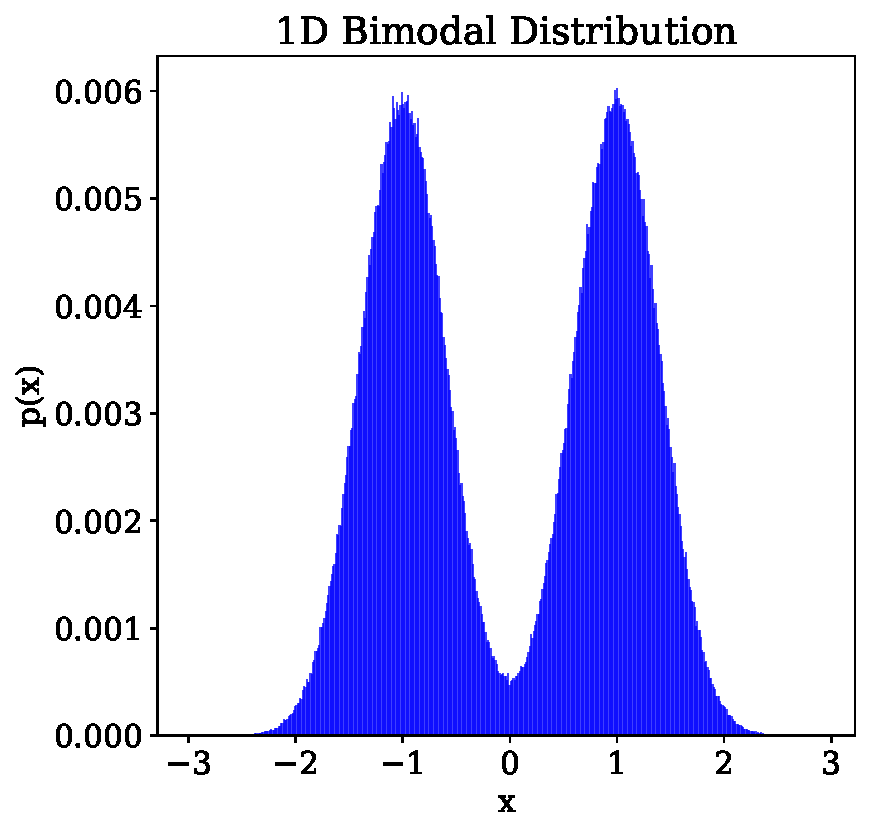
\includegraphics[height=\textwidth]{figures/chapter-09/1d_bimodalplot.pdf}
        \caption{}
        \label{fig:otherdistributions_1Di}
    \end{subfigure}
    \begin{subfigure}[b]{0.4\textwidth}
        \centering
        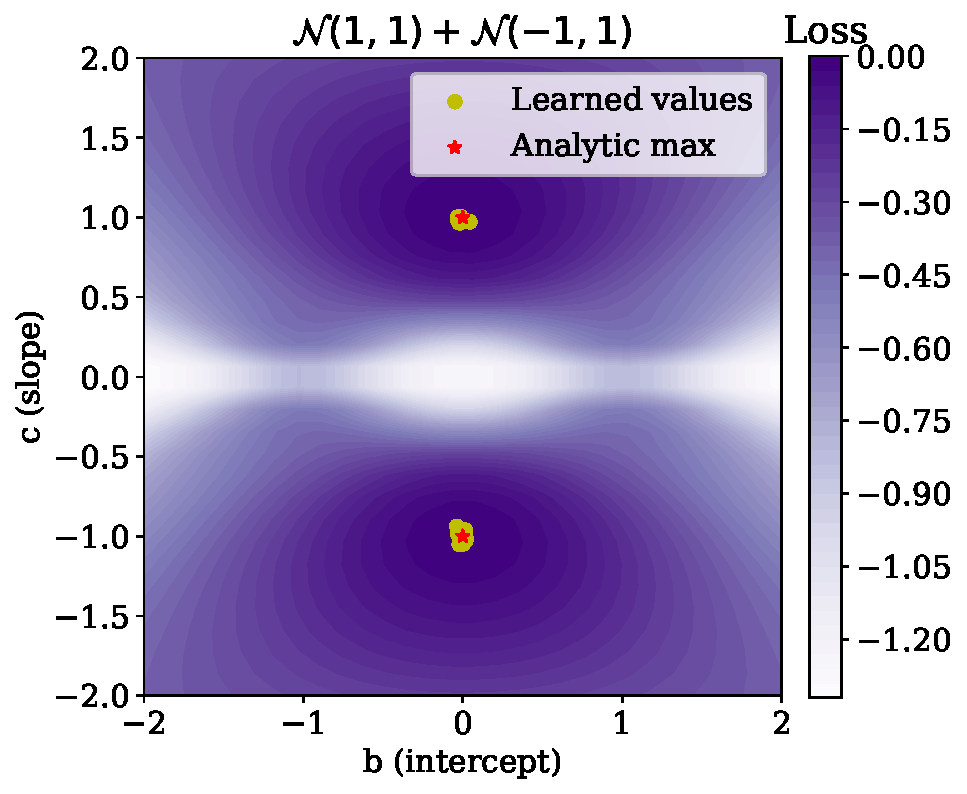
\includegraphics[height=\textwidth]{figures/chapter-09/1d_bimodalsymm.pdf}
        \caption{}
        \label{fig:otherdistributions_1Dii}
    \end{subfigure}
    \caption[\textsc{SymmetryGAN}'s predictions for a bimodal Gaussian mixture with $\mathbb{Z}_2$ reflection symmetry and corresponding loss landscape validation.]{Symmetry discovery for a one dimensional bimodal Gaussian mixture $p(x) = \frac{1}{2}\mathcal{N}(-1, 1) + \frac{1}{2}\mathcal{N}(1, 1)$ possessing $\mathbb{Z}_2$ symmetry. (a) Probability density function showing two symmetric modes at $x = \pm 1$ with equal weights and variances, creating a distribution invariant under reflection about the origin. (b) Analytic loss landscape in the $(b, c)$ parameter space for linear transformations $g(x) = b + cx$, with empirically discovered symmetries overlaid (blue points). The landscape exhibits two distinct maxima at $(b, c) = (0, 1)$ and $(0, -1)$, corresponding to the identity and reflection transformations respectively. The discovered symmetries cluster precisely at these theoretical optima, confirming that \textsc{SymmetryGAN} correctly identifies the cyclic group $\mathbb{Z}_2 = \{x \mapsto \pm x\}$ as the complete symmetry group of the distribution.}
    \label{fig:otherdistributions-1D}
\end{figure}
\begin{figure}
    \centering
    \begin{subfigure}[b]{0.27\textwidth}
        \centering
        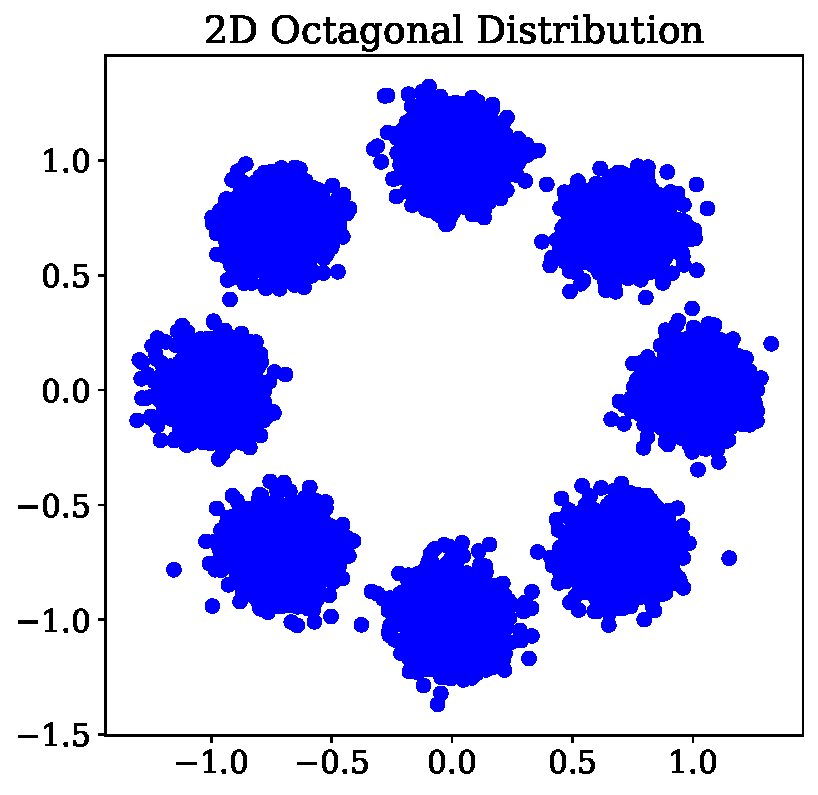
\includegraphics[height=\textwidth]{figures/chapter-09/2d_circularplot.pdf}
        \caption{}
        \label{fig:otherdistributions_2D_i}
    \end{subfigure}
    \hfill
    \begin{subfigure}[b]{0.28\textwidth}
        \centering
        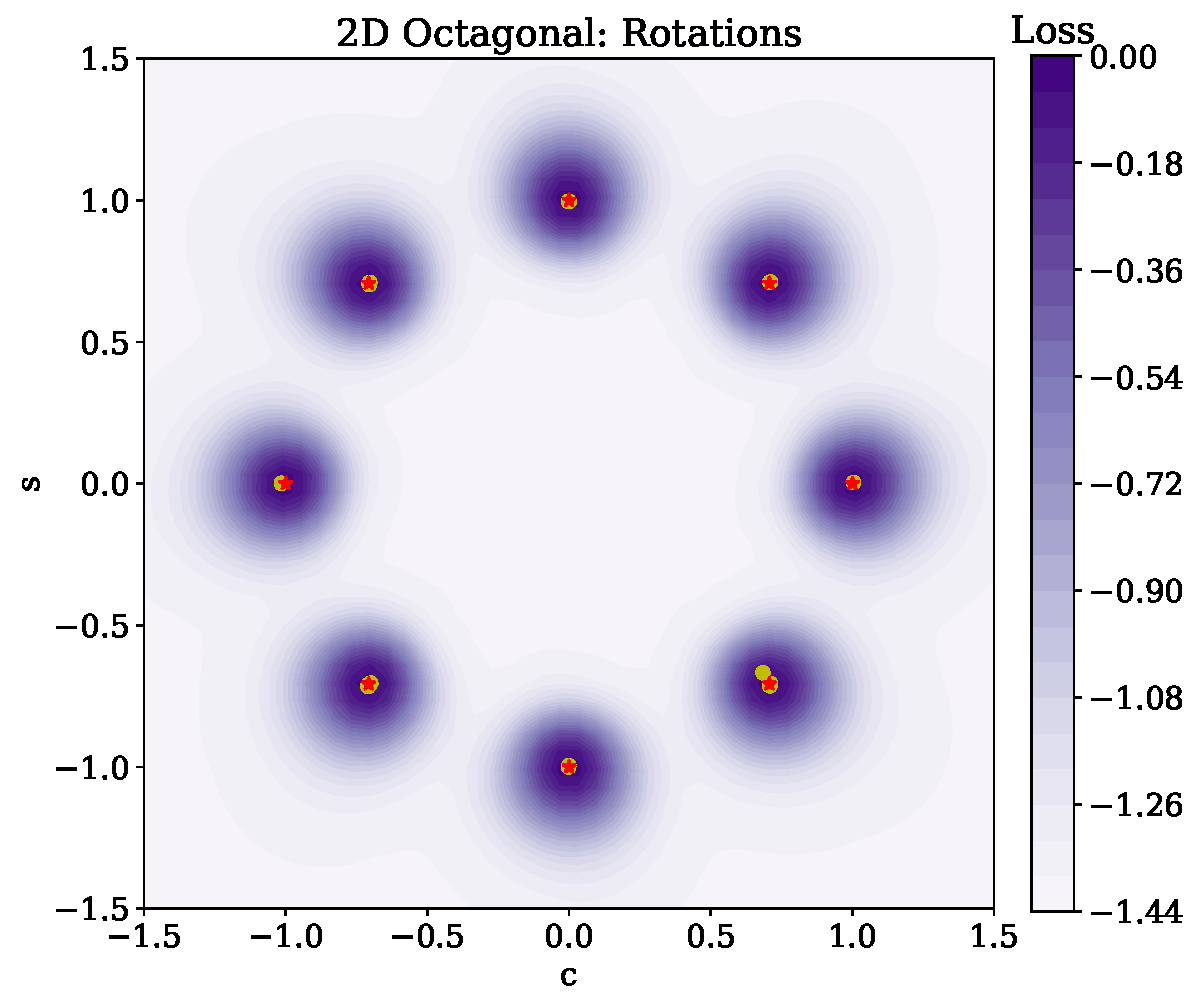
\includegraphics[height=\textwidth]{figures/chapter-09/2doctagonalrotations.pdf}
        \caption{}
        \label{fig:otherdistributions_2D_ii}
    \end{subfigure}
    \hfill
    \begin{subfigure}[b]{0.27\textwidth}
        \centering
        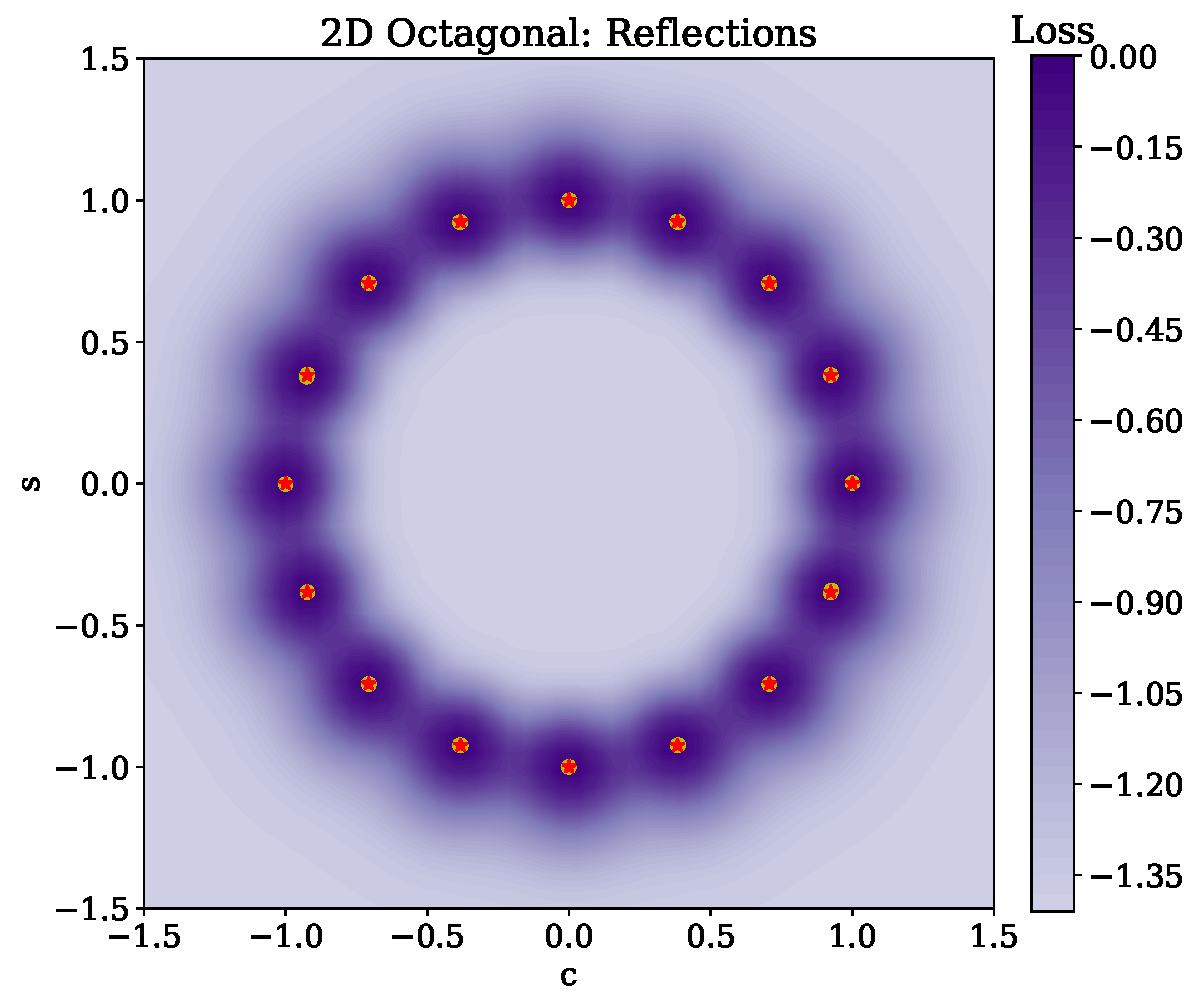
\includegraphics[height=\textwidth]{figures/chapter-09/2doctagonalreflections.pdf}
        \caption{}
        \label{fig:otherdistributions_2D_iii}
    \end{subfigure}
    
    \vspace{0.3cm}
    
    \begin{subfigure}[b]{0.27\textwidth}
        \centering
        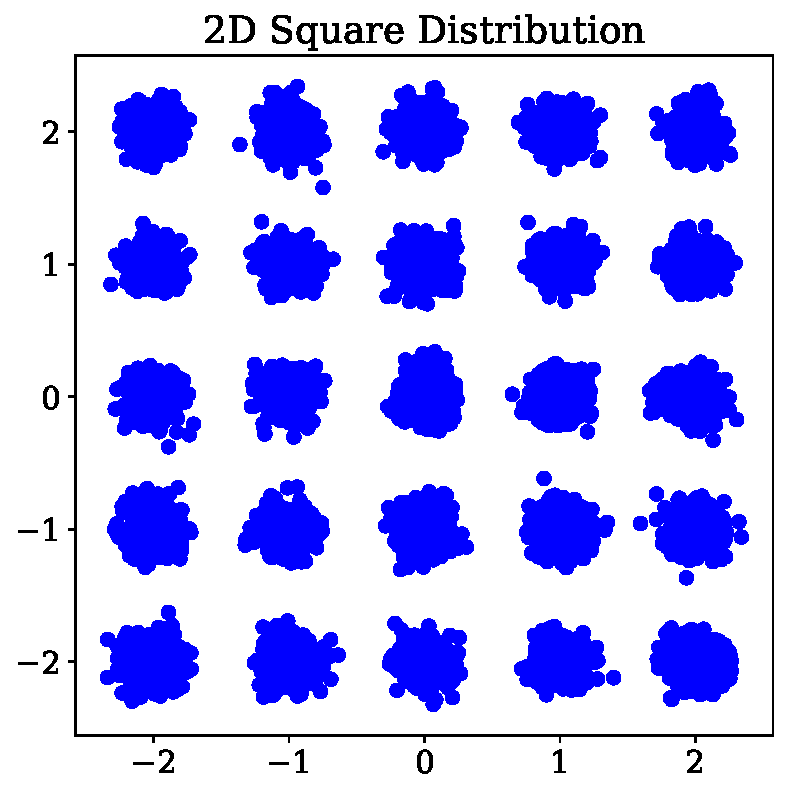
\includegraphics[height=\textwidth]{figures/chapter-09/2d_squareplot.pdf}
        \caption{}
        \label{fig:otherdistributions_2D_iv}
    \end{subfigure}
    \hfill
    \begin{subfigure}[b]{0.28\textwidth}
        \centering
        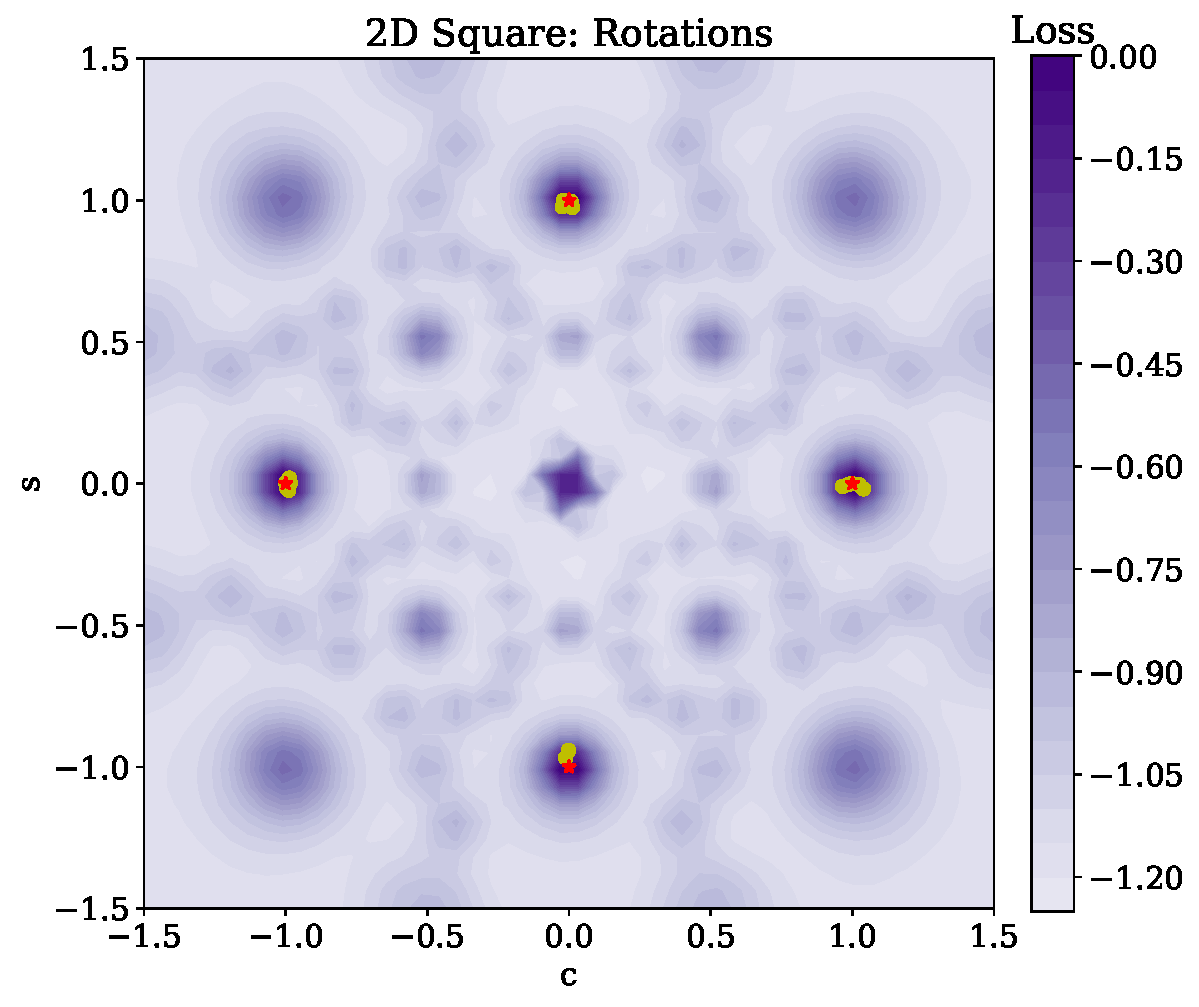
\includegraphics[height=\textwidth]{figures/chapter-09/2dsquarerotations.pdf}
        \caption{}
        \label{fig:otherdistributions_2D_v}
    \end{subfigure}
    \hfill
    \begin{subfigure}[b]{0.27\textwidth}
        \centering
        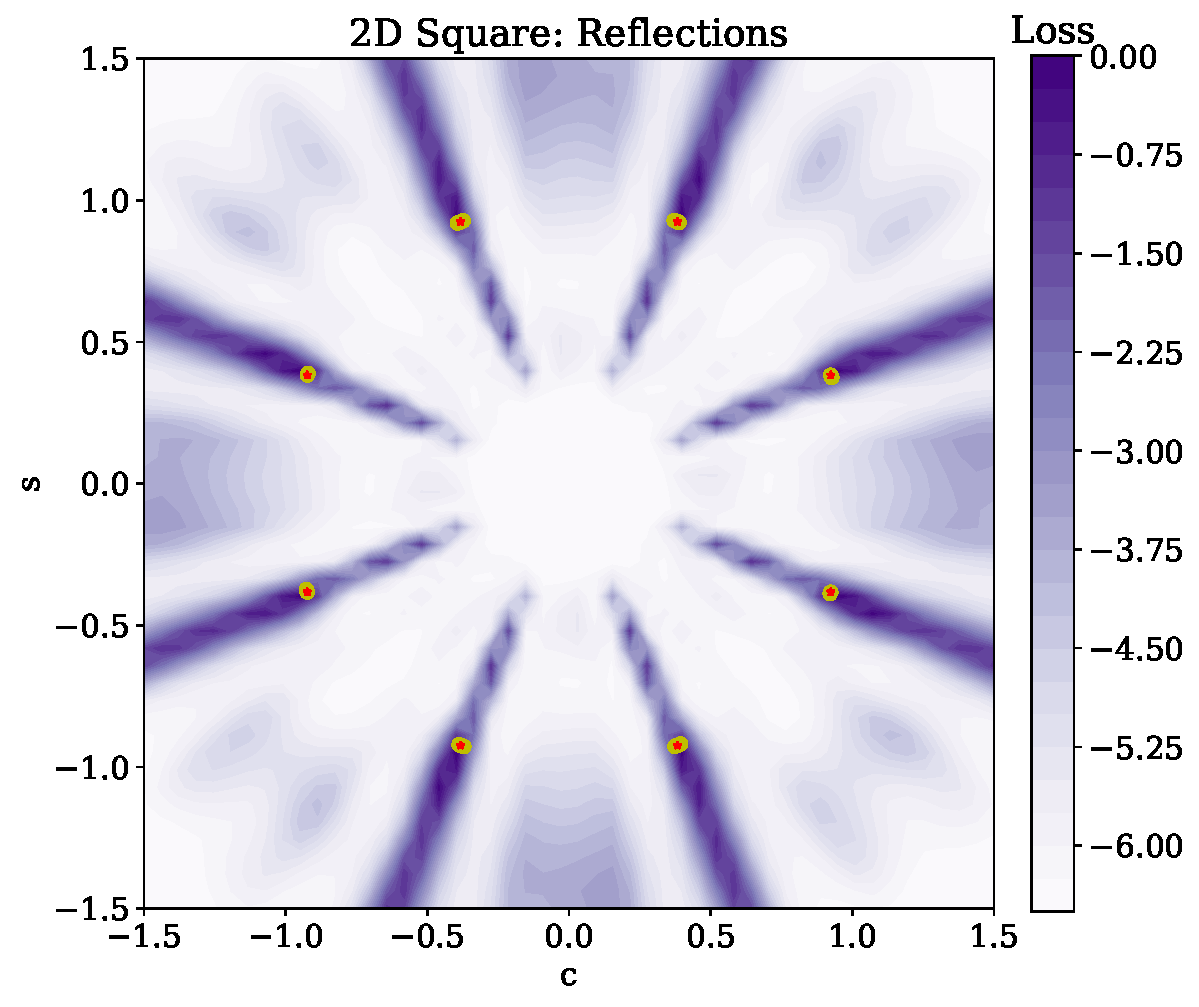
\includegraphics[height=\textwidth]{figures/chapter-09/2dsquarereflections.pdf}
        \caption{}
        \label{fig:otherdistributions_2D_vi}
    \end{subfigure}
    
    \caption[Discovery of dihedral symmetries $D_8$ and $D_4$ in octagonal and square lattice Gaussian mixtures.]{Symmetry discovery for two dimensional Gaussian mixture models with non-commutative discrete symmetry groups. Top row: Octagonal distribution $p(\mathbf{x}) = \frac{1}{8}\sum_{k=0}^{7} \mathcal{N}(\mathbf{\mu}_k, 0.1\mathbbm{1})$ where $\mathbf{\mu}_k = (\cos\frac{2\pi k}{8}, \sin\frac{2\pi k}{8})$, possessing dihedral symmetry $D_8$. (a) Probability density showing eight equally-spaced modes on the unit circle. (b) Discovered rotations cluster at multiples of $\frac{\pi}{4}$, corresponding to the eight rotational symmetries. (c) Discovered reflections appear at eight angles, with antipodal points representing the same reflection axis. Bottom row: Square lattice distribution $p(\mathbf{x}) = \frac{1}{25}\sum_{i,j=-2}^{2} \mathcal{N}((i,j), 0.1\mathbbm{1})$ with dihedral symmetry $D_4$. (d) Probability density showing a $5 \times 5$ grid of Gaussian modes. (e) Discovered rotations concentrate at $0, \frac{\pi}{2}, \pi, \frac{3\pi}{2}$, identifying the four rotational symmetries. (f) Discovered reflections cluster at four angles corresponding to horizontal, vertical, and diagonal reflection axes. The precise alignment of discovered symmetries with theoretical predictions demonstrates \textsc{SymmetryGAN}'s ability to identify complex non-commutative groups.}
    \label{fig:otherdistributions-2D}
\end{figure}
                The second is a two dimensional octagonal distribution,
                \[
                    p(x) = \frac{1}{8}\sum_{i=1}^{8} \mathcal{N}(\cos\frac{2\pi i}{8}, 0.1)\times \mathcal{N}(\sin\frac{2\pi i}{8}, 0.1)
                \]
                which has the dihedral group \(D_8\) as its symmetry group, a non-commutative discrete group containing both rotations and reflections.
                %
                The third is a \(5\times 5\) square distribution,
                \[
                    p(x) = \frac{1}{25}\sum_{i=0}^{4}\sum_{j=0}^{4} \mathcal{N}(i-2, 0.1)\times \mathcal{N}(j-2, 0.1)
                \]
                which has the dihedral group \(D_4\) as its symmetry group, also a non-commutative discrete group containing both rotations and reflections.
                %
                The left column of \cref{fig:otherdistributions-2D} shows data from each of these distributions, the middle column shows the discovered rotations, and the right column shows the discovered reflections.
                %
                In each case \textsc{SymmetryGAN} is able to correctly discover the symmetries of the distribution.

        \subsection{Particle physics experiments.}
            
            The transition from Gaussian toy models to HEP data represents a significant increase in complexity.

            This study focuses on dijet data.
            %
            Jets are the collimated streams of hadrons that emerge when high energy quarks or gluons undergo fragmentation, and two jet final states constitute one of the dominant signatures recorded at the LHC.
            
            Given an infrared- and collinear-safe clustering algorithm, every jet is assigned a unique 4--momentum;
            %
            The ensuing kinematic ensemble permits a systematic search for symmetries in the momentum distributions.

            This analysis employs the background dijet sample released for the LHC Olympics anomaly-detection challenge \cite{Kasieczka:2021xcg,kasieczka_rd_2019}.
            %
            Parton showering and hadronisation are simulated with \textsc{Pythia} 8.219 \cite{Sjostrand:2007gs}, while detector effects are modelled using \textsc{Delphes} 3.4.1 \cite{DeFavereau2014DELPHESExperiment,Mertens:2015kba}.
            %
            Final state particles reconstructed by \textsc{Delphes} are clustered into anti$-k_T$ jets with radius parameter $R=1$ using \textsc{FastJet} 3.3.0 \cite{Cacciari:2008gp,Cacciari2008TheAlgorithm,Cacciari2012FastJetManual}.
            %
            Events must pass a single jet trigger requiring $p_T>\num{1.2}{\TeV}$;
            %
            the subsequent analysis is restricted to the two highest$-p_T$ jets in each event, where transverse momentum is defined by $p_T=\sqrt{p_x^{2}+p_y^{2}}$.
\begin{figure}
    \centering
    \begin{subfigure}[b]{0.4\textwidth}
        \centering
        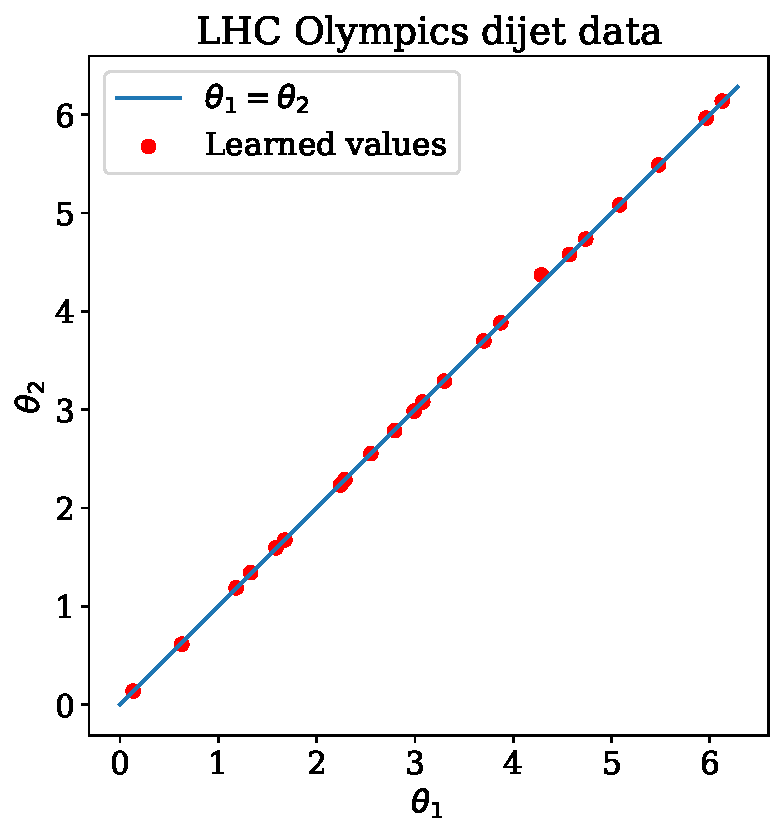
\includegraphics[height=\textwidth]{figures/chapter-09/LHCO.pdf}
        \caption{}
        \label{fig:LHCO_i}
    \end{subfigure}
    \begin{subfigure}[b]{0.4\textwidth}
        \centering
        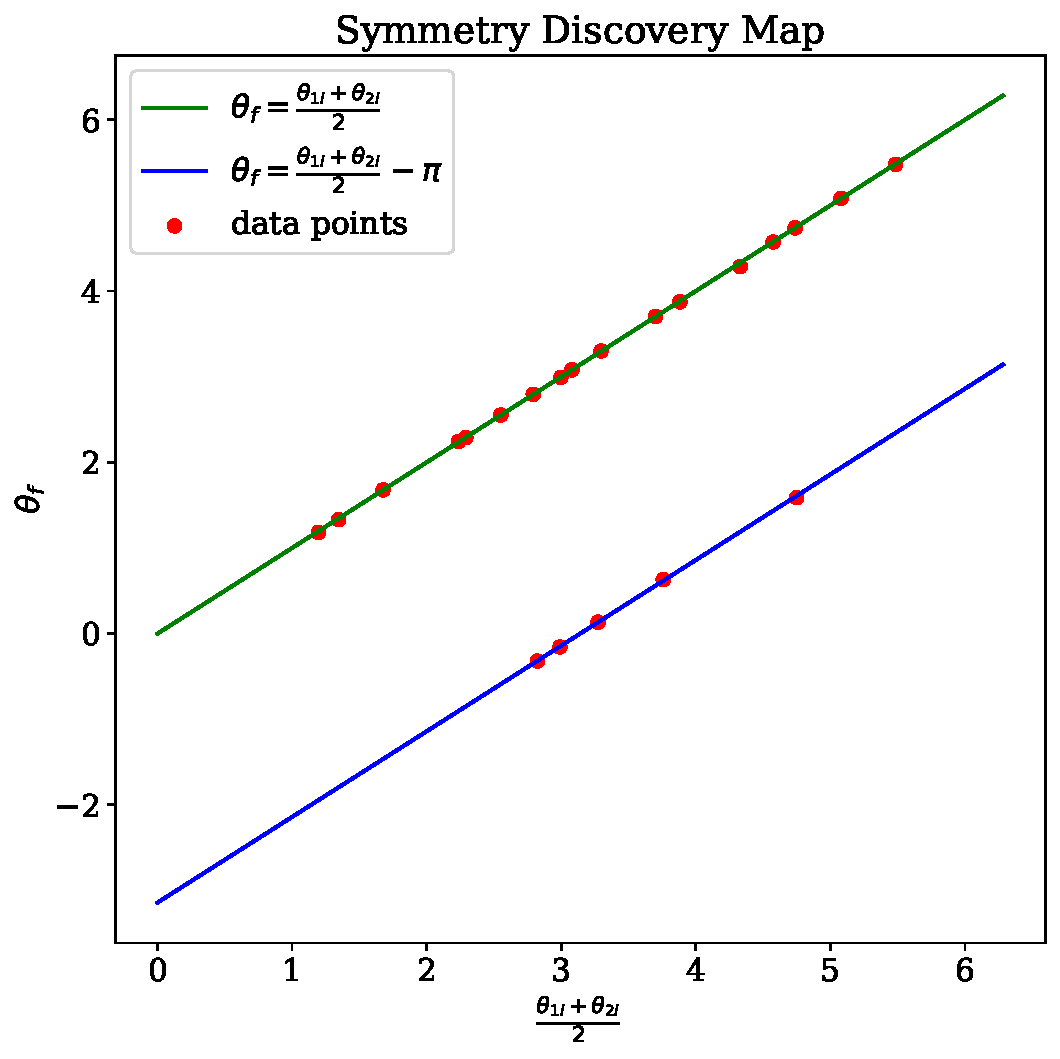
\includegraphics[height=\textwidth]{figures/chapter-09/LHCO_avg.pdf}
        \caption{}
        \label{fig:LHCO_ii}
    \end{subfigure}
    \caption{Symmetry discovery on transverse momenta of dijet events using \textsc{SymmetryGAN} with a $SO(2) \times SO(2)$ search space, where each jet undergoes independent azimuthal rotation $g_{\theta_1,\theta_2}(\mathbf{p}) = (R(\theta_1)\mathbf{p}_1, R(\theta_2)\mathbf{p}_2)$. (a) Distribution of converged parameters $(\theta_1^f, \theta_2^f)$ from independent training runs initialised uniformly in $[0, 2\pi)^2$. The discovered symmetries cluster along the diagonal $\theta_1 = \theta_2$ (blue line), confirming that only simultaneous rotations preserve the dijet distribution, a direct consequence of transverse momentum conservation. (b) Symmetry discovery map $\Omega: (\theta_1^i, \theta_2^i) \mapsto \theta^f$ revealing the loss landscape dynamics. The final rotation angle follows $\theta^f = \frac{\theta_1^i + \theta_2^i}{2}$ when $|\theta_1^i - \theta_2^i| < \pi$ (shown in green), and $\theta^f = \frac{\theta_1^i + \theta_2^i}{2} - \pi$ when $|\theta_1^i - \theta_2^i| > \pi$ (shown in blue). This bisection rule represents the path of steepest ascent in the loss landscape, demonstrating how gradient dynamics naturally discover the physical constraint without prior knowledge.}
    \label{fig:LHCO}
\end{figure}
           This experiment was also repeated on the transverse momenta of dijet events from CMS Open Data~\cite{komiske_cms_2019}.
           %
           \textsc{SymmetryGAN} produced similar results on both datasets.
            
            Each event is characterised by the transverse momentum components
            \[
                \mathbf{x} = (p_{1x}, p_{1y}, p_{2x}, p_{2y})
            \]
            The initial exploration considers transformations from \(SO(2) \times SO(2)\), independently rotating each jet in the transverse plane.
            %
            The generator is restricted to the block diagonal form
            \[
                g_{\theta_1,\theta_2}(\mathbf{x}) = \begin{bmatrix}
                    R(\theta_1) & 0 \\
                    0 & R(\theta_2)
                \end{bmatrix} \mathbf{x}
            \]
            %
            Momentum conservation predicts that only simultaneous rotations \(\theta_1 = \theta_2\) should preserve the distribution.
            %
            The empirical results confirm this beautifully: starting from random initializations in \([0, 2\pi)^2\), the learned parameters cluster along the diagonal \(\theta_1 = \theta_2\).
            %
            \cref{fig:LHCO_i} shows the discovered symmetries for the \(SO(2) \times SO(2)\) case.
            %
            The symmetry discovery map for this system reveals unexpected elegance.
            %
            The mapping from initial to final parameters follows:
            \[
                \Omega(\theta_1, \theta_2) = \begin{cases}
                    \frac{\theta_1 + \theta_2}{2} & |\theta_1 - \theta_2| < \pi \\
                    \frac{\theta_1 + \theta_2}{2} - \pi & |\theta_1 - \theta_2| > \pi
                \end{cases}
            \]
            %
            This bisection of the angular difference represents the path of steepest ascent in the loss landscape, demonstrating how gradient dynamics naturally discover the constraint imposed by momentum conservation, illustrated in \cref{fig:LHCO_ii}.
\begin{figure}
    \centering
    \begin{subfigure}[b]{0.4\textwidth}
        \centering
        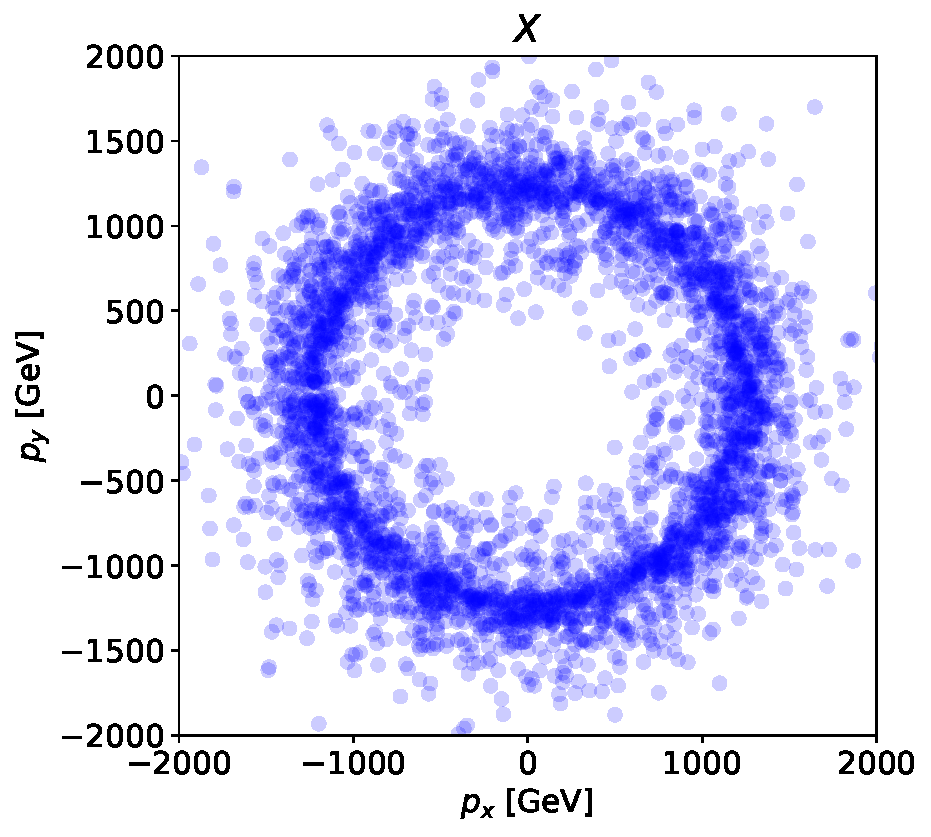
\includegraphics[width=\textwidth]{figures/chapter-09/LHCO_Comparison1.pdf}
        \caption{}
        \label{fig:LHCOComparison_i}
    \end{subfigure}
    \hfill
    \begin{subfigure}[b]{0.4\textwidth}
        \centering
        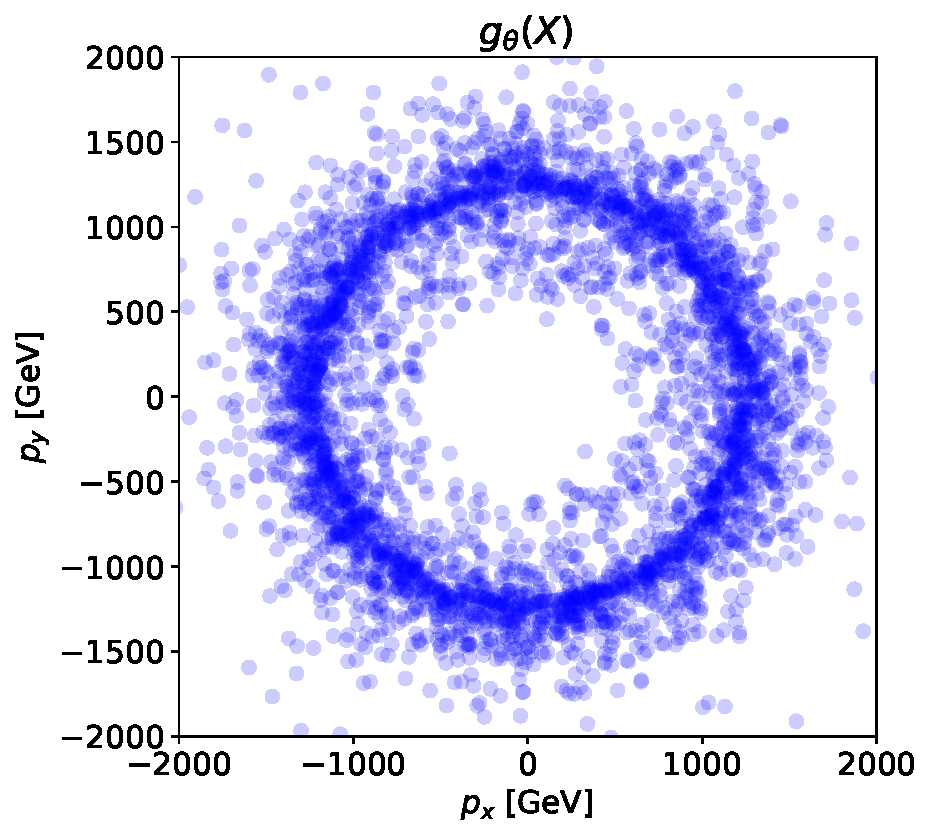
\includegraphics[width=\textwidth]{figures/chapter-09/LHCO_Comparison2.pdf}
        \caption{}
        \label{fig:LHCOComparison_ii}
    \end{subfigure}
    \caption[Visual validation of discovered dijet symmetry through transverse momentum preservation.
]{Visual validation of discovered symmetry in dijet events through transverse momentum distributions. (a) Original LHC Olympics showing the two leading jets' momenta $(p_x, p_y)$ in the transverse plane. The circular structure reflects the detector's azimuthal symmetry. (b) Same events transformed by a discovered generator from \textsc{SymmetryGAN}, showing identical statistical properties. The preservation of the ring structure and angular distribution confirms that the discovered transformation represents a genuine symmetry of the dijet system. Each point represents one event.}
    \label{fig:LHCO_Comparison}
\end{figure}

\begin{figure}
    \centering
    \begin{subfigure}[b]{0.45\textwidth}
        \centering
        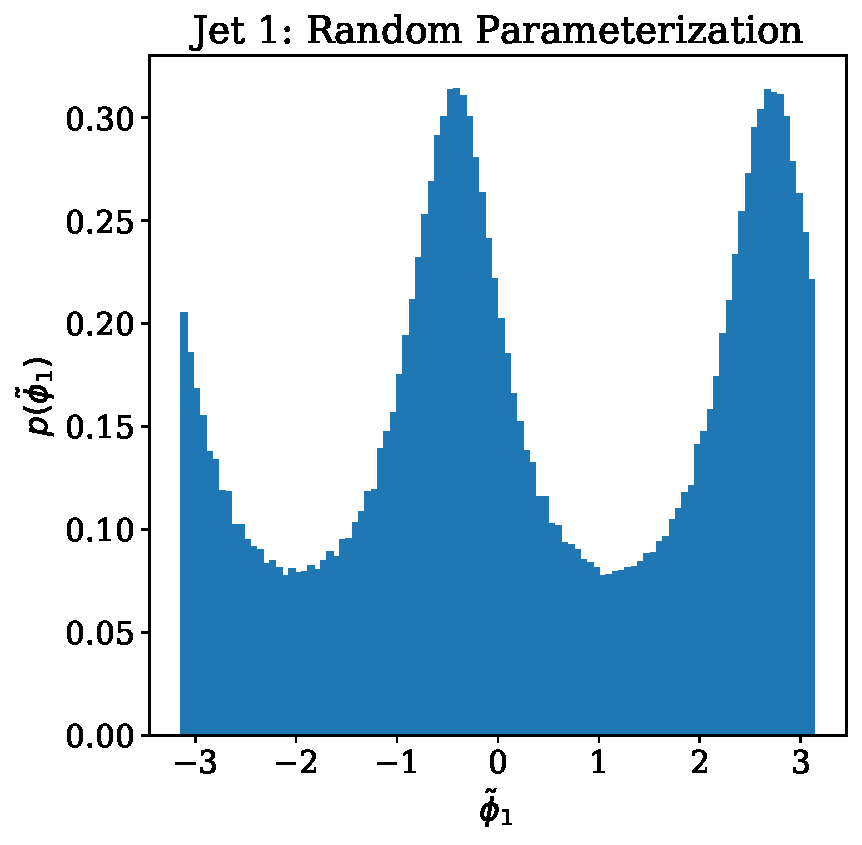
\includegraphics[width=\textwidth]{figures/chapter-09/KL_rand1.pdf}
        \caption{}
        \label{fig:KLrand_i}
    \end{subfigure}
    \hfill
    \begin{subfigure}[b]{0.45\textwidth}
        \centering
        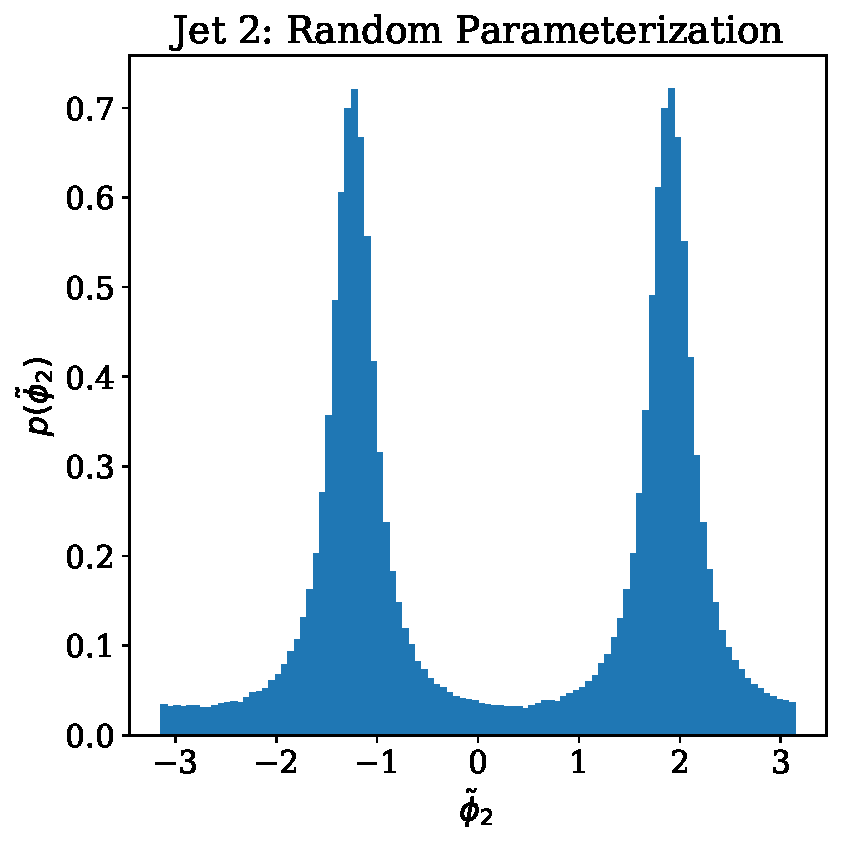
\includegraphics[width=\textwidth]{figures/chapter-09/KL_rand2.pdf}
        \caption{}
        \label{fig:KLrand_ii}
    \end{subfigure}
\\
    \begin{subfigure}[b]{0.45\textwidth}
        \centering
        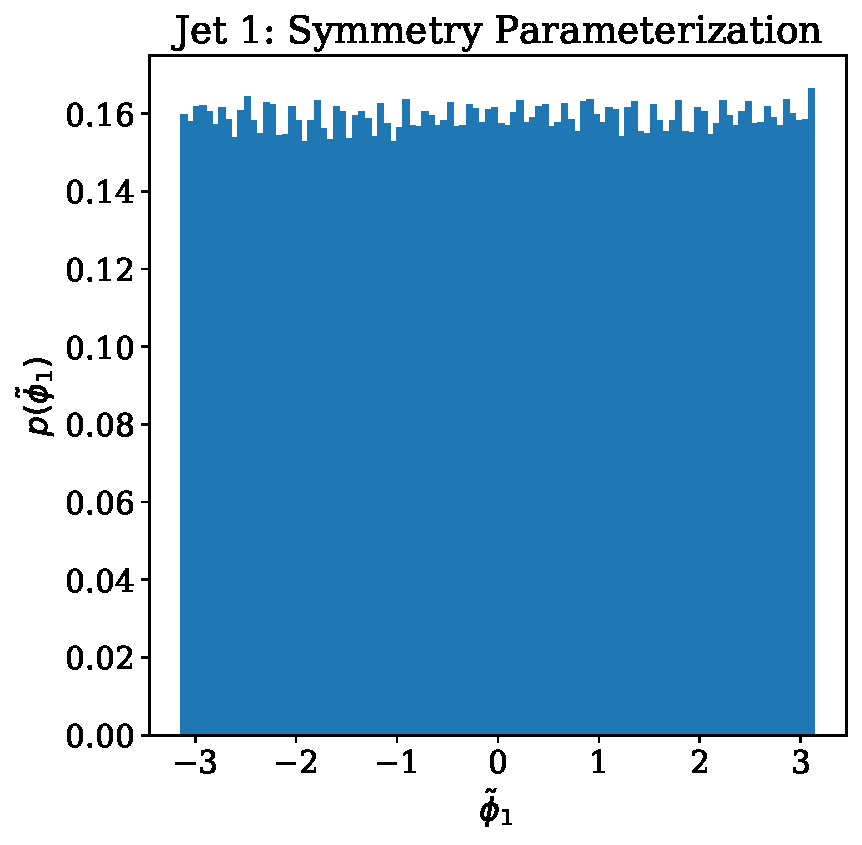
\includegraphics[width=\textwidth]{figures/chapter-09/KL_symm1.pdf}
        \caption{}
        \label{fig:KLsymm_i}
    \end{subfigure}
    \hfill
    \begin{subfigure}[b]{0.45\textwidth}
        \centering
        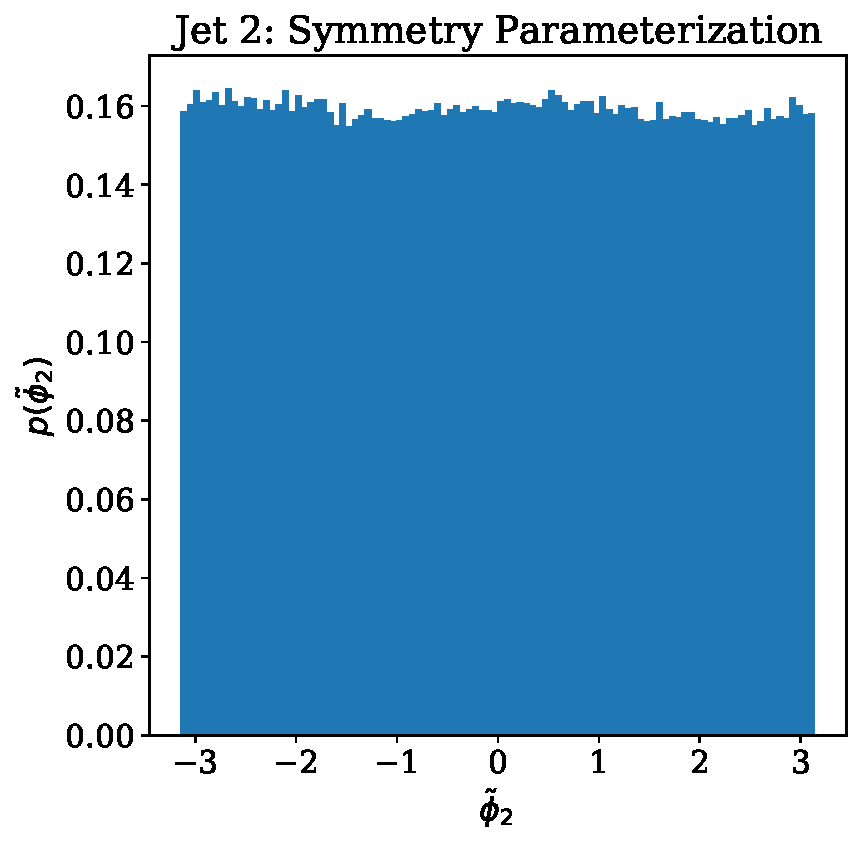
\includegraphics[width=\textwidth]{figures/chapter-09/KL_symm2.pdf}
        \caption{}
        \label{fig:KLsymm_ii}
    \end{subfigure}
    \caption[Non-uniform azimuthal distributions from random $SO(4)$ rotations demonstrating symmetry violation, and uniform azimuthal distributions from discovered symmetry confirming invariance of dijet system.]
    {(a) and (b) Azimuthal angle distributions after applying a random $SO(4)$ rotation to dijet events, demonstrating violation of symmetry. Transformed azimuthal angles $\tilde{\phi}_1, \tilde{\phi}_2$ exhibits clear non-uniformity. The Kullback-Leibler divergence $D_{KL}(p||\mathcal{U}) \approx 0.15$ quantifies this deviation from uniformity, confirming that arbitrary $SO(4)$ rotations do not preserve the dijet distribution. This serves as a negative control for the symmetry discovery algorithm.
    (c) and (d) Azimuthal angle distributions after applying a discovered symmetry transformation, validating the symmetry discovery. Transformed azimuthal angle $\tilde{\phi}_1, \tilde{\phi}_2$ exhibit uniformity within statistical fluctuations. $D_{KL}(p||\mathcal{U}) < 10^{-2}$ confirms near-perfect agreement with the uniform distribution.}
    \label{fig:KL_rand_and_sym}
\end{figure}

             
            Expanding to the full \(SO(4)\) search space introduces greater complexity.
            %
            An arbitrary element of \(SO(4)\) is the composition of six independent rotations, in the six possible orthogonal \(2-\)planes.
            %
            The six parameter group does not admit a simple visualisation, and the discovered symmetries no longer lie in any two or three dimensional subspace.
            %
            Validation requires more sophisticated statistical tests.
            
            Visual inspection can, however, serve as a smell test.
            %
            Projections of the original and transformed distributions onto physically meaningful observables (jet \(p_T\), azimuthal angles) show excellent agreement \cref{fig:LHCO_Comparison}.
            %
            Having passed the visual test, one can now apply more discerning tests to ensure the symmetries are not spurious.
            %
            The transformed azimuthal angles
            \[
                \mqty[\tilde{\phi}_1\\\tilde{\phi}_2] = \mqty[
                    \arctan \frac{g(\theta_1, \theta_2)(p_{1y})}{g(\theta_1, \theta_2)(p_{1x})} \\
                    \arctan \frac{g(\theta_1, \theta_2)(p_{2y})}{g(\theta_1, \theta_2)(p_{2x})}
                ]
            \]
            %
            are uniformly distributed only for true symmetries, and not for any other transformation, as shown in \cref{fig:KL_rand_and_sym}.
\begin{figure}
    \centering
    \begin{subfigure}[b]{0.45\textwidth}
        \centering
        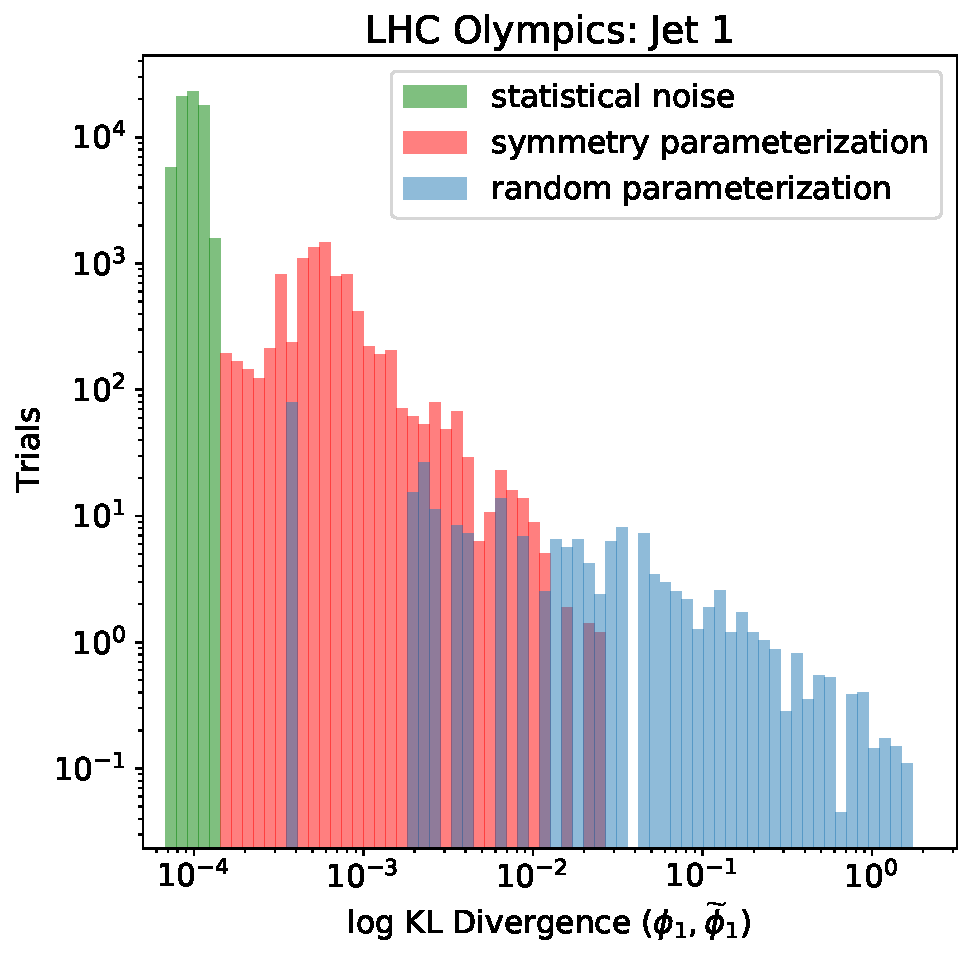
\includegraphics[width=\textwidth]{figures/chapter-09/KL_Div1.pdf}
        \caption{}
        \label{fig:KLdiv_i}
    \end{subfigure}
    \hfill
    \begin{subfigure}[b]{0.45\textwidth}
        \centering
        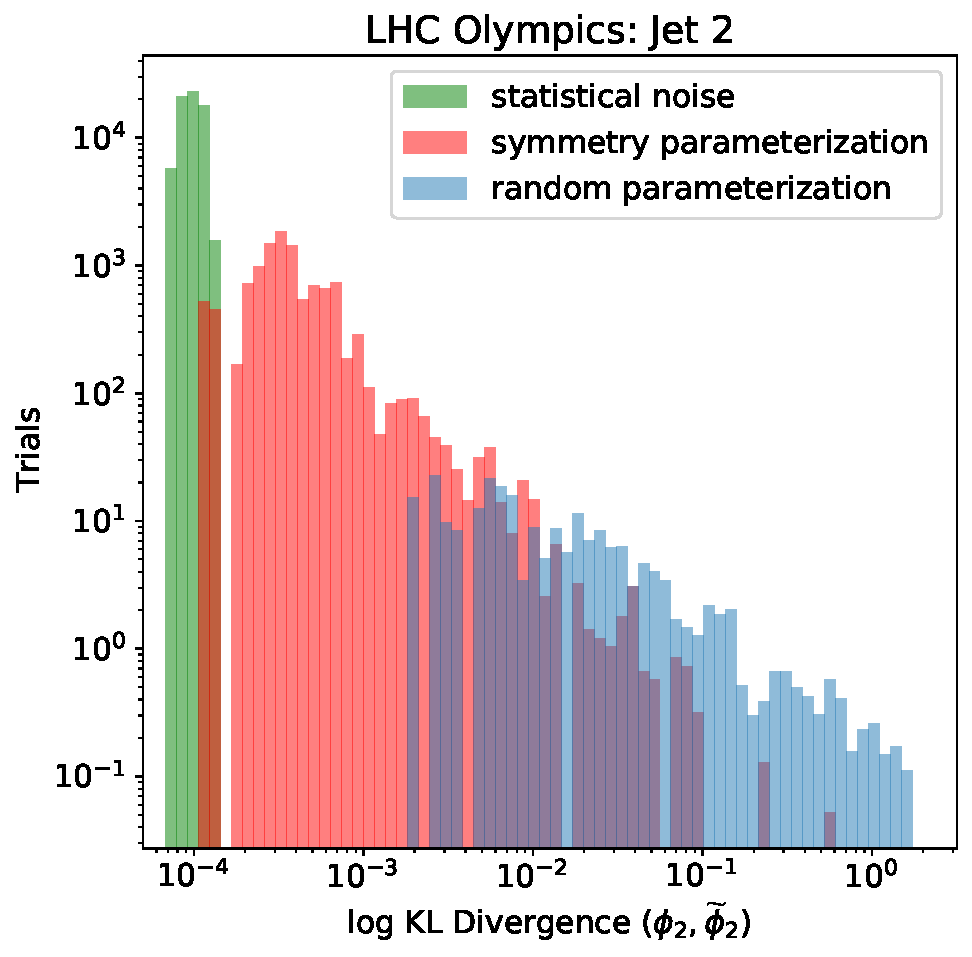
\includegraphics[width=\textwidth]{figures/chapter-09/KL_Div2.pdf}
        \caption{}
        \label{fig:KLdiv_ii}
    \end{subfigure}
    \caption[Kullback-Leibler divergence analysis showing discovered symmetries approach statistical noise floor.]{Quantitative validation of discovered symmetries via Kullback-Leibler divergence analysis. Histograms show $D_{KL}(\phi || \tilde{\phi})$ between original and transformed azimuthal angle distributions for (a) leading jet and (b) subleading jet. Three distinct populations emerge: discovered symmetries (red) with means of 0.0058 and 0.0090 respectively, approaching the irreducible statistical noise floor (green) at $D_{KL} \approx 10^{-3}$ arising from finite sample size. Random $SO(4)$ rotations (blue) exhibit significantly higher divergences with means of 0.37 and 0.34, confirming they violate the symmetry. Note the logarithmic scale emphasises the low divergence region.}
    \label{fig:KL-symm}
\end{figure}

\begin{figure}
    \centering
    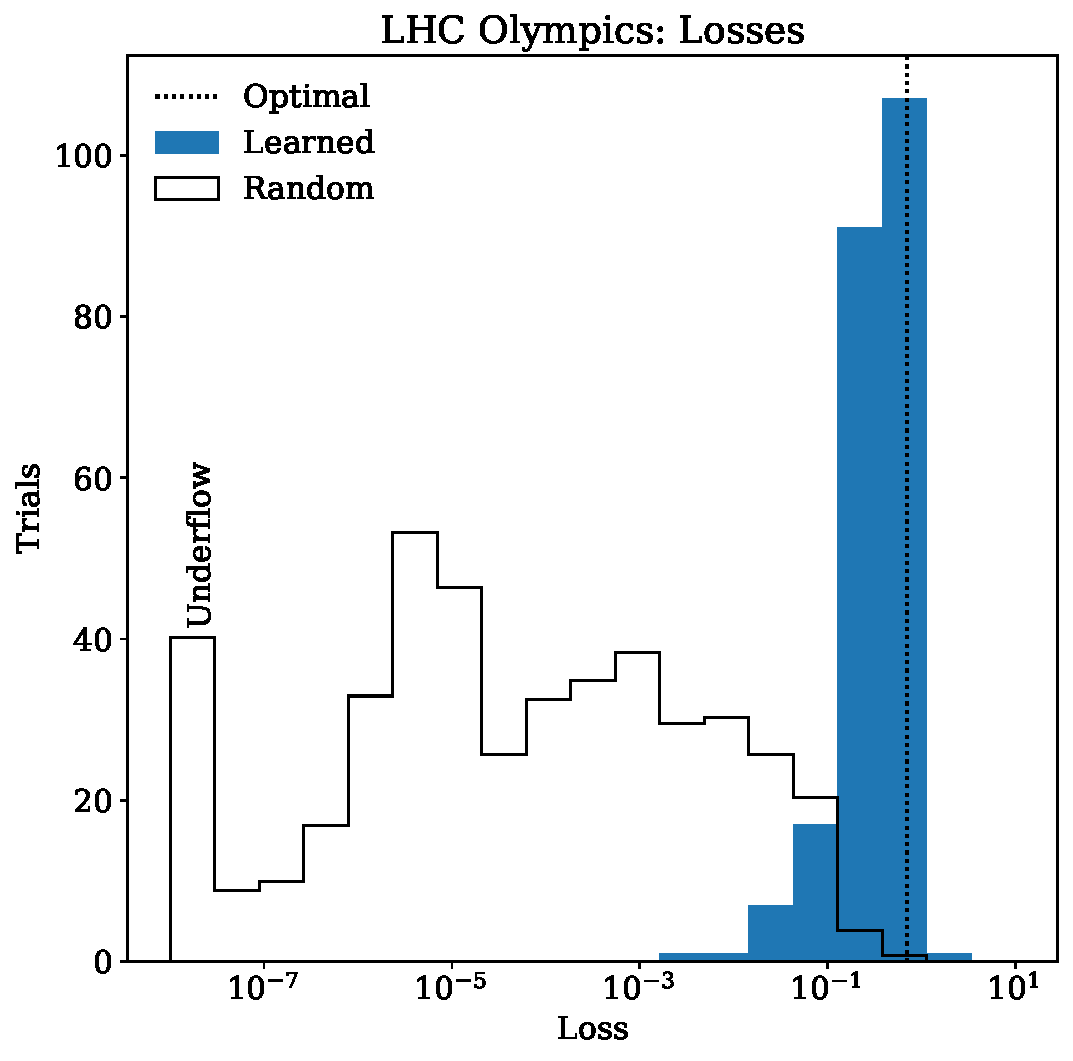
\includegraphics[width=0.6\textwidth]{figures/chapter-09/LHCOLosses.pdf}
    \caption{Discriminator loss distributions validating discovered symmetries against theoretical optimum. The histogram shows \textit{ post hoc} discriminator losses when trained to distinguish original from transformed dijet events. Discovered symmetries (blue) achieve losses tightly clustered around $2\log 2 \approx 1.386$ (dashed line), the theoretical minimum for perfect symmetries where transformed and original distributions are indistinguishable.
    %
    Random $SO(4)$ rotations (black) yield significantly lower losses, indicating the discriminator easily identifies these as non-symmetries. The discovered transformations achieve losses within 1\% of the theoretical optimum, providing independent confirmation that \textsc{SymmetryGAN} identifies genuine invariances of the dijet system without prior physics knowledge.}
    \label{fig:LHCOLosses}
\end{figure}            
            Computing the KL divergence between the transformed and original distributions is another way to test for symmetry.
            %
            The KL divergence should be zero for true symmetries, and non-zero for any other transformation.
            %
            While this is never exactly true, \cref{fig:KL-symm} shows the KL divergence for true symmetries approach the irreducible statistical noise floor.
            
            Finally, \textit{post hoc} discriminators trained on discovered transformations achieve losses within 1\% of the theoretical optimum \(2\log 2\) confirming these represent genuine symmetries, illustrated in \cref{fig:LHCOLosses}.
            %
            The discovered subgroup of \(SO(4)\) includes the expected \(SO(2)\) rotations reflecting cylindrical detector geometry, but also unexpected combinations that would be difficult to identify through physical intuition alone.
            
        \subsection{Interpreting discovered symmetries.}
            The interpretation of discovered symmetries requires bridging the gap between abstract mathematical transformations and physical understanding.
            %
            This translation process reveals both the power and limitations of automated symmetry discovery.
            
            Each discovered symmetry transformation corresponds to a conservation law or invariance principle in the underlying physics.
            %
            For the dijet system, the discovered azimuthal rotations connect directly to angular momentum conservation about the beam axis.
            %
            The continuous \(SO(2)\) symmetry reflects the absence of any preferred direction in the transverse plane---a fundamental consequence of the cylindrical geometry of both the collision process and the detector.
            
            More subtle are the discovered discrete symmetries.
            %
            The non-\(SO(2)\) transformations found combine specific overall rotations with jet exchanges.
            %
            For example,
            \[
                g_{Z_2}(p_{1x}, p_{1y}, p_{2x}, p_{2y}) = (-p_{2x}, -p_{2y}, -p_{1x}, -p_{1y})
            \]
            is a transformation that simultaneously rotates by \(\pi\) and exchanges the two jets---a symmetry that follows from the identical nature of QCD jets but may not be obvious without a systematic search.        
            %
            The relationship between discovered symmetries and known physics provides crucial validation.
            %
            Each symmetry found by \textsc{SymmetryGAN} corresponds to either:
            \begin{itemize}
                \item A fundamental symmetry of physics (Lorentz invariance, gauge symmetry)
                \item A symmetry of the experimental setup (cylindrical detector geometry)
                \item An emergent symmetry from kinematic constraints (momentum conservation)
            \end{itemize}
            %
            No spurious symmetries appear, demonstrating the method's reliability.
            
            The next challenge in this space is: how does one move from discovering individual symmetry transformations to understanding the complete symmetry group structure?

\section{Towards symmetry inference.}
            The distinction between symmetry discovery and symmetry inference represents a fundamental challenge in the \textsc{SymmetryGAN} framework.
            %
            While the method excels at finding individual elements of a symmetry group, reconstructing the complete group structure requires additional theoretical machinery.
            
            The task of symmetry inference can be formulated as ``Given a set of discovered symmetry transformations \(\{g_1, g_2, ..., g_n\}\), determine the minimal group \(G\) containing all these elements.''
            %
            Three complementary approaches emerge for tackling this challenge.
            \begin{enumerate}
                \item \textbf{Discrete subgroup analysis}: By modifying the loss function to enforce specific algebraic relations, \textsc{SymmetryGAN} can systematically probe for discrete subgroups.
                %
                \textsc{SymmetryGAN} trained with the cyclic group constraint, \cref{eq:cyclic-loss}, successfully identifies \(Z_q\) subgroups within larger symmetry groups, as seen in \cref{fig:MSE}.
                %
                This approach extends naturally to other discrete groups through appropriate constraint terms, though non-Abelian groups require more sophisticated loss modifications.
                \item \textbf{Group composition methods}: The closure property of groups suggests an iterative approach: given discovered symmetries \(\{g_i\}\), compute all possible compositions \(g_i \circ g_j\) to expand the known group elements.
                %
                For continuous groups like \(SO(2)\), a single irrational rotation angle generates a dense subgroup, effectively recovering the entire group through composition~\cite{hall_matrix_2015}.
                %
                However, numerical precision limits this approach.
                %
                Each composition compounds errors, leading to degradation after multiple iterations.
                %
                The practical limit appears to be \numrange{10}{20} compositions before accumulated errors overwhelm the signal.
                \item \textbf{The Symmetry Discovery Map}: Perhaps the most promising direction involves learning the complete mapping from initialisation space to symmetry space:
                \[
                    \Omega: \mathbb{R}^k \rightarrow \mathcal{G}
                \]
                where \(\mathcal{G}\) represents the symmetry group manifold.
                %
                This map encodes the complete symmetry structure implicitly, as its image is precisely the symmetry group.
                %
                Preliminary attempts to learn \(\Omega\) had limit success.
                %
                The main challenges are that the map must begin near the identity to preserve the connection between initial and final parameters, and the min--max nature of GAN training becomes more complex when optimising over maps on the space of transformations rather than transformations themselves.
                %
                Despite these challenges, successful learning of even approximate symmetry discovery maps would provide a powerful tool to characterise symmetry groups.
            \end{enumerate}

\section{Symmetry informed unfolding}
\label{sec:symmetry-informed-unfolding}
    The fundamental challenge of unfolding, recovering truth level distributions from detector smeared observations, stems from its ill posed nature.
    %
    Multiple truth distributions can yield identical observations after detector effects, creating an underdetermined system primed for additional constraints.
    %
    Symmetry provides a natural regularisation scheme for unfolding problems.
    %
    When a physical process respects a symmetry, that invariance constrains the space of valid solutions, effectively regularising the inverse problem without introducing artificial biases.
    %
    Consider the standard unfolding problem formulated as an optimisation,
    \[
        \min_{p(z)} \left[ \chi^2\qty{p(x), \int r(x\mid z) \, p(z)\,\dd z} + \lambda \cdot \mathcal{R}(p(z)) \right]
    \]
    where \(r\) represents is detector response and \(\mathcal{R}\) is a regularisation term.
    %
    Traditional approaches use generic smoothness penalties, but symmetries provide physically motivated constraints.
    %
    For a symmetry group \(G\) discovered through \textsc{SymmetryGAN}, one could construct the symmetry preserving regularisation,
    \[
        \mathcal{R}_\text{sym}(p) = \sum_{g \in G} \left\| p - g \cdot p \right\|^2
    \]
    %
    This penalty vanishes for distributions respecting the symmetry while penalizing asymmetric solutions.
    %   
    Such a regularisation term would enforce invariances that the underlying physics demands rather than imposing arbitrary smoothness constraints.
    
    However such an implementation would have to address subtle challenges.
    %
    For continuous symmetries like \(SO(2)\), the sum over group elements becomes an integral requiring careful handling.
    %
    A possible solution is to select group elements that uniformly cover the symmetry manifold.
    %
    For \(SO(2)\), for instance, one could sample angles \(\theta_i = 2\pi i/N\) for \(i = 0, ..., N-1\).
    %
    However, any such choice would be \textit{ad hoc} and would introduce artifacts into the unfolding process, because one would be treating the data as though it had the symmetry \(\mathbb{Z}_N\) rather than \(SO(2),\) in this example.

    For non-compact groups, the challenge is further compounded by the fact that there no longer exists a equivariant sampling strategy in the first place.
    %
    Methods such as importance sampling based on data distribution do exist~\cite{goertzel_quota_1949}, but they remain to be tested in the physics context.
    
    The theoretical foundation of this approach connects to information theory.
    %
    Each symmetry represents a constraint reducing the effective dimensionality of the solution space.
    %
    For a distribution over \(N\) bins with a \(\mathbb{Z}_k\) cyclic symmetry, the degrees of freedom reduce from \(N\) to \(N/k\), improving the effective statistics by a factor of \(k\).
    %
    This dimensionality reduction should translate directly to improved unfolding stability.

    \subsection{Symmetry preserving neural network architectures.}
        The architectural encoding of symmetries represents a paradigm shift from \textit{post hoc} constraints to intrinsic guarantees.
        %
        \begin{definition}
        A neural network \(f_\theta\) is said to be \textit{equivariant} under the action group \(G\) on its input space \(X\) if
        \[
            \forall g\in G\quad\forall x\in X\quad\,f_\theta(g \cdot x) = g \cdot f_\theta(x)
        \]
        \end{definition}
        For unfolding applications, one could seek architectures where the mapping from observed to truth level distributions preserves known symmetries.
        %
        The Group Convolutional Neural Network (G-CNN) framework provides one example of such an approach~\cite{Cohen:2016wkb}.
        %
        For a symmetry group \(G\) acting on the input space, G-CNN layers take the form
        \[
            f * \psi = \int_H f(h)\psi(g^{-1}h) dh
        \]
        where \(*\) denotes group convolution and \(h\in H\) is the stabilizer subgroup.
        %
        This formulation guarantees equivariance by construction, not training.

        The LGN (Lorentz Group Network) architecture~\cite{Bogatskiy:2020tje} constructs features from Lorentz scalars and 4--vectors in order to preserve Lorentz invariance.
        %
        For identical particle handling, Deep Sets~\cite{Zaheer:2017wmg} and Set2Graph~\cite{Serviansky:2020qwa} provide principled approaches in which
        \[
            f(\{x_1, ..., x_n\}) = \rho\left(\sum_i \phi(x_i)\right)
        \]
        where \(\phi\) and \(\rho\) are learned functions, guaranteeing invariance to particle ordering.
        
        For processes involving gauge bosons, architectures must respect gauge transformations.
        %
        The Gauge Equivariant Mesh CNN~\cite{haan_gauge_2021} provides a framework for \(SU(3) \times SU(2) \times U(1)\) invariance.

        A hybrid architecture for symmetry aware unfolding could combine these elements.
        %
        The architecture would then necessarily ensure that certain symmetries would be present in the unfolded distribution.
        %
        However, the practical implementation of such an architecture remains an open question.
    \subsection{Reducing dimensionality through symmetry identification.}
        The curse of dimensionality poses a significant challenge for unfolding problems, especially for binned approaches.
        %
        Each additional degree of freedom exponentially increases the dimension of the solution space, degrading statistical power and amplifying instabilities.
        %
        Symmetry identification offers a principled method for revealing redundancies that can be eliminated without information loss.
        
        For a distribution with symmetry group \(G\), the effective dimensionality of the distribution can be reduced from the ambient space dimension to the dimension of the quotient space \(X/G\).

        \begin{definition}
        A function \(f: X \rightarrow \mathbb{R}\) is \(G\)-\textbf{invariant} if and only if there exists a function \(\tilde{f}: X/G \rightarrow \mathbb{R}\) with \(f = \tilde{f} \circ \pi\) where \(\pi: X \rightarrow X/G\) is the canonical projection.
        \end{definition}
        
        This factorisation is the key to dimensionality reduction.
        %
        One needs only unfold \(\tilde{f}\) on the lower--dimensional quotient space.
        
        The statistical gain from this procedure scales dramatically with dimensionality.
        %
        For a \(d\)-dimensional space with a \(k\)-parameter continuous symmetry group, the effective dimensionality reduces to \(d-k\), yielding an effective statistics increase of
        \[
            N_{\text{eff}} = \frac{N}{C_d}
        \]
        where \(C_d\) is a complexity measure (e.g. covering number~\cite{shalev-shwartz_understanding_2014}, VC dimension~\cite{vapnik_uniform_1971}, local intrinsic dimensionality~\cite{tempczyk_lidl_2022}, or metric entropy~\cite{20166.1Uses}).
        %
        Dimensionality reduction reduces \(C_d\), which increases \(N_{\text{eff}}\).
        %
        Any such process of symmetry based projection, however, requires careful treatment of statistical uncertainties.
        
        \subsection{Hidden symmetries and emergent simplicity.}
            Often, the most powerful dimensionality reductions come from unexpected symmetries.
            %
            The discovery of approximate custodial symmetry in electroweak physics simplified phenomenology dramatically.
            %
            Similarly, emergent symmetries in complex physical ensembles can enable radical dimensionality reduction~\cite{schmalian_emergent_2008}.

            The quantitative impact of symmetry based dimensionality reduction admits a rigorous mathematical treatment.
            \subsubsection{Formalism}
            \begin{definition}[{\(G\)-Equivariant Fisher Information}]
                For a likelihood \(\mathcal L(x\mid\theta)\) whose parameter space carries an action of a finite or Lie group \(G\), the \emph{\(G\)-equivariant Fisher information matrix} is  
                \[
                  \bigl[\mathcal I_G(\theta)\bigr]_{ij}
                  \;=\;
                  \mathbb E\!\Bigl[
                      \frac{\partial\log \mathcal L}{\partial\theta_i}
                      \frac{\partial\log \mathcal L}{\partial\theta_j}
                  \Bigr]
                  \;-\;
                  \sum_{g\in G} w_g\,
                  \mathbb E\!\Bigl[
                      \frac{\partial\log \mathcal L}{\partial\theta_i}
                      \frac{\partial\log \mathcal L(g \cdot \theta)}{\partial\theta_j}
                  \Bigr],
                \]
                where \(\{w_g\}_{g\in G}\) are averaging weights satisfying \(\sum_{g\in G}w_g=1\).  Equivalently,  
                \(\mathcal I_G(\theta)=P_G\,\mathcal I(\theta)\,P_G^{T}\) where \(P_G\) is the orthogonal projection operator onto the \(G\)-invariant subspace~\cite{nielsen_elementary_2020}.
\end{definition}
\begin{theorem}[Symmetry-Adapted Cramér–Rao Bound~\cite{Cramer1946MathematicalStatistics, RadhakrishnaRao1945InformationParameters, rao_selected_1994, darmois_sur_1945, aitken_xvestimation_1942, deming_letters_1970}]
    Let \(\hat\theta\) be any unbiased estimator of \(\theta\in\mathbb R^d\) based on \(N\) i.i.d.\ samples, and assume the statistical model \(p(x\mid\theta\) is \(G\)-equivariant.
Then the covariance matrix obeys the lower bound
\[
  \operatorname{Cov}(\hat\theta)
  \;\succeq\;
  \frac{1}{N}\,\mathcal I_G^{-1}(\theta),
\]
where \(\succeq\) denotes the Loewner partial order.  The lower bound is saturated if and only if the score vectors projected onto the invariant subspace are linear in \((\hat\theta-\theta)\).
\end{theorem}

\begin{proof}[Proof sketch.]
The classical information inequality states that
\(\operatorname{Cov}(\hat\theta)\succeq N^{-1}\mathcal I^{-1}(\theta)\).
Because the model and the estimator respect the group action, both sides commute with \(P_G\).  
Projecting the score function onto the invariant subspace and using \(P_G^2=P_G\) yields  
\(\operatorname{Cov}(\hat\theta)\succeq N^{-1}(P_G\mathcal I P_G)^{-1}=N^{-1}\mathcal I_G^{-1}\,\).
\end{proof}

\begin{corollary}[Variance Reduction for Finite Symmetries]
For a discrete group \(G\) of order \(|G|\) and a scalar parameter, if  
\[\rho=\frac{\mathbb{E}\qty[\pdv{\log \mathcal L}{\theta}\pdv{\log \mathcal L\circ g}{\theta}]}
          {\mathbb{E}\qty[\qty(\pdv{\log L}{\theta})^2]}
\] for the average pairwise correlation of score functions across group orbits,  
then
\[
  \frac{\operatorname{Var}(\hat\theta_{\text{sym}})}
       {\operatorname{Var}(\hat\theta_{\text{unconstrained}})}
  \;=\;
  \frac{1}{|G|}+\frac{|G|-1}{|G|}\,\rho.
\]
This means that symmetry is maximally beneficial (\(\rho \to 0\)) when orbit scores are uncorrelated, recovering the \(1/|G|\) ideal reduction factor.
\end{corollary}

When \(G\) is continuous, replacing the group sum with Haar integration yields an integral projector and analogous results.
%
The practical implication is that enforcing equivariance in unfolding algorithms tightens the attainable RMS by precisely the factor dictated by group averaged score correlations.


    \subsection{Applications for unfolding jet substructure variables.}
        Consider unfolding jet substructure observables like N-subjettiness ratios \(\tau_{21}\).
        %
        The IRC safety of these observables implies approximate scale invariance.
        %
        For a scaling symmetry with parameter \(\lambda\):
        \[
            \tau_{21}(\lambda p_T, \lambda m_\text{jet}) = \tau_{21}(p_T, m_\text{jet})
        \]
        This symmetry reduces the 2D unfolding problem in \((p_T, m_\text{jet})\) to a 1D problem in the ratio \(m_\text{jet}/p_T\).
        %
        The maximal possible theoretical precision gain is
        \[
            \sigma_{\tau_{21}}^\text{sym} = \frac{\sigma_{\tau_{21}}^\text{2D}}{\sqrt{\log(p_T^\text{max}/p_T^\text{min})}}.
        \]
        For typical jet \(p_T\) ranges spanning a few orders of magnitude, this offers a tangible improvement in precision.

        Such analyses also provides additional insights.
        %
        Each symmetry can theoretically reduce the Kullback--Leibler divergence between truth and reconstructed distributions by as much as
        \[
            \Delta D_{KL} = \frac{1}{2} \log |G| - \frac{1}{2N} \text{Tr}(\mathcal{I}_G^{-1} \mathcal{I}_\text{unconstrained})
        \]
        This reduction could directly translate to improved unfolding fidelity, with larger symmetry groups yielding greater gains.

        Such thought experiments point toward a broader principle.
        %
        The most powerful machine learning approaches for physics don't just learn from data but incorporate fundamental physical principles into their architecture.
        %
        Discovering and enforcing symmetries can transforms unfolding from a purely statistical exercise into a physics informed inference problem, achieving results that respect both the data and the underlying theoretical framework.

\section{Improved precision using symmetries}
\label{sec:improved-measurement-prediction}
    The transformation of symmetry from abstract mathematical concept to concrete measurement tool represents one of the most profound opportunities in modern particle physics analysis.
    %
    This section speculates about how integrating symmetry awareness and unfolding might affect the ability to extract truth from data.
    %
    These ideas, while not yet implemented, are intended to reflect on potential future directions that translate discovered invariances into measurement precision.
    \subsection{Data augmentation using discovered symmetries.}
        The concept of data augmentation through symmetry sits at the intersection of theoretical physics and practical statistics.
        %
        The flip side of the dimensionality reduction discussed in \cref{sec:symmetry-informed-unfolding} is that when a dataset respects certain transformations, the effective statistics of that dataset can be multiplied without collecting a single additional event.
        %
        This is not merely a computational trick, it reflects a deep truth about the information structure of symmetric systems.

        Symmetry based data augmentation is the process of generating statistically equivalent synthetic data by applying discovered symmetry transformations to existing events, effectively increasing sample size while preserving all physical properties.
        %
        Traditional data augmentation in machine learning often relies on heuristic transformations.
        %
        These modifications hope to capture invariances without formal guarantees.
        %
        By contrast, symmetry based augmentation leverages proven invariances discovered through methods like \textsc{SymmetryGAN}.
        %
        Every augmented event is, by construction, as physically valid as the original.

        As with the dimension reduction discussed in \cref{sec:symmetry-informed-unfolding}, the the sampling strategy can introduce challenges.
        %
        For finite groups, one might include all group elements, and for compact continuous groups so long as one samples carefully from the uniform measure on the group manifold to avoid bias, the artifacts introduced will, in the very least, be unbiased.
        %
        For non-compact groups, the uniform measure is not well defined, and there is no way to guarantee that the artifacts introduced are unbiased.

        The power of symmetry based augmentation extends beyond simple counting statistics.
        %
        Symmetry augmentation can heal detector defects.
        %
        Imagine a calorimeter module at \(\phi = \pi/2\) suffering from reduced efficiency.
        %
        With symmetry augmentation, one can rotate events from healthy detector regions to fill the gap:

        The corrected distribution would be given by
        \[
            n_{\text{corrected}}(\phi = \pi/2) = \frac{1}{|G|} \sum_{g \in G} \epsilon(g^{-1} \cdot \phi) \cdot n_{\text{observed}}(g^{-1} \cdot \phi)
        \]
        where \(\epsilon(\phi)\) represents the \(\phi-\)dependent efficiency.
        %
        This is more than mere interpolation.
        %
        It is the use of physical symmetry to transport information across phase space.

        The interplay with machine learning architectures reveals another dimension.
        %
        Neural networks trained on symmetry augmented data should exhibit
        \begin{itemize}
            \item \textbf{Faster convergence}: The effective sample size increase should translate directly to fewer training epochs.
            \item \textbf{Better generalisation}: The network `sees' the full symmetry orbit during training, preventing overfitting to specific configurations.
            \item \textbf{Automatic equivariance}: Even non-equivariant architectures should learn equivariant information from augmented data.
        \end{itemize}
        
        For all the benefits that symmetry aware augmentation might provide, not all symmetries admit straightforward augmentation.
        %
        Even with simple discrete symmetries like a \(\mathbb{Z}_2\) while one can invert event coordinates, care is needed with derived quantities.
        %
        Or for instance, a jet clustering algorithm might produce different multiplicities when applied to parity reflected events, breaking the supposed equivalence.
        %
        In this sense the augmentation must respect the full analysis chain, not just the raw kinematics, and symmetries that admit all the steps of the analysis chain are, naturally, more difficult to find.

    \subsection{Symmetry constrained unfolding.}
        A variant of moment unfolding where the functional basis is restricted to symmetry respecting functions could guide choices of basis functions grounded in physical principles.
        %
        \cref{chap:moment-unfolding} discussed the \(p_T\) dependent Boltzmann--like basis functions, \(\vb*{\beta}_a(p_T)\), which were approximated as linear functions of jet \(p_T\),
        \[
            \vb*{\beta}_a(p_T) = {\beta}_a^{(0)} + {\beta}_a^{(1)}\,p_T,
        \]
        to constrain the flexibility of the generator network.
        %
        A symmetry aware parametrisation of the \(\vb*{\beta}_a(p_T)\) could provide a more principled way to constrain the generator network, while still achieving the necessary regularisation.
        
        Implementing a similar approach in RAN architectures would requires careful attention to the increased complexity of the architecture, but a symmetry aware regularisation scheme could provide improved conditioning, by making the response matrix block--diagonal in symmetry sectors, and imposing physical consistency constraints where unfolded distributions automatically respect, for example, IRC safety, providing smoothness within symmetry sectors without violating invariance.

        The quantitative impact of symmetry awareness on measurement precision admits rigorous analysis through the lens of information theory and statistical estimation.
        %
        The information content of data about parameters \(\theta\) under symmetry group \(G\) is captured by the equivariant Fisher information matrix \(\mathcal{I}_G(\theta)\), which bounds the achievable precision of any unbiased estimator.
        %
        The fundamental result stems from the Equivariant Cramér-Rao Bound discussed in \cref{sec:symmetry-informed-unfolding}.
        
        In addition, symmetry awareness provides more than variance reduction.
        %
        It fundamentally alters the bias-variance tradeoff.
        %
        Traditional unfolding must balance bias from regularisation and variance from statistical fluctuations.
        
        Symmetry constraints modify the bias-variance tradeoff,
        \[
            \text{Bias}_{\text{sym}} = \frac{\text{Var}_0}{n \cdot S(\mathcal{G})}
        \]
        where \(S(\mathcal{G})\) is the `symmetry factor' quantifying variance reduction, so that the total error becomes
        \[
            \text{MSE}_{\text{total}} = \text{Bias}_{\text{sym}}^2 + \frac{\text{Var}_0}{n \cdot S(\mathcal{G})}.
        \]
        In this sense, symmetry aware unfolding is not only about improved statistics, but also about extracting the maximum physical information from finite data.

\section{Conclusion}
\label{sec:symmetrygan-conclusion}
    This chapter began with the seemingly simple question of what it means for a dataset to possess symmetry, only to wade layers of mathematical formalism involving Jacobian factors, inertial reference densities, and the interplay between statistical and physical invariances.
    %
    This final section looks forward to new territory ready for exploration.

    \subsection{Beyond linear symmetries.}
        The restriction to affine equiareal maps, while yielding impressive results, also represents a clear limitation of current analyses.
        %
        Nature's symmetries extend far beyond the affine group, encompassing transformations that twist, fold, and reshape phase space in ways that linear maps cannot capture.
        %
        Consider the H\'enon map~\cite{ibanez_simple_1976}, a deceptively simple area preserving transformation,
        \[
            g(x,y) = (x, y - x^2)
        \]
        It is but one of a vast and relatively uncharted space of the full (nonlinear) \emph{equiareal group}.
        %
        The structure of the equiareal group is complex enough to allow for a rich theory of symmetries and their associated invariances with the right computational tools.
        
        In particle physics, such transformations emerge naturally, and are ubiquitous, from the rapidity transformation in relativistic kinematics, to the symplectic structure imposed by Poisson brackets on classical phase space and the corresponding commutation relations of quantum mechanics.
        %
        Normalising flows, on account of their bijective nature, could be a natural fit for exploring symplectic geometries and their associated symmetries.
        %
        That said, the greater challenge lies not in the architecture but in the search space.
        %
        Linear transformations form a finite dimensional Lie group, amenable to systematic exploration.
        %
        Non-linear symplectic maps form an infinite dimensional space that lacks a known parametrisation or classification.
        %
        Recent work on Hamiltonian neural networks~\cite{greydanus_hamiltonian_2019} suggests one possible path to describe transformations through generating functions that automatically preserve symplectic structure.
        
        A few examples of particle physics applications of non-linear symmetries are
        \begin{itemize}
            \item \textbf{Jet substructure}: The Lund plane reveals approximate scale invariant symmetries best expressed through logarithmic transformations~\cite{Dreyer:2018nbf}.
            \item \textbf{Heavy flavor physics}: Dalitz plot analyses exhibit non-linear symmetries from resonance dynamics~\cite{Asner:2003gh}.
            \item \textbf{Multiparticle correlations}: Collective flow in heavy ion collisions follows non-linear hydrodynamic symmetries~\cite{Yan:2015lwn}.
        \end{itemize}
        The path forward requires synergy between differential geometry, machine learning, and physics intuition, a synthesis that will push the boundaries of all three fields.
    
    \subsection{Approximate symmetries and symmetry breaking.}
        Perfect symmetries, while mathematically elegant, rarely survive contact with experimental reality.
        %
        The universe abounds in approximate symmetries---patterns that almost hold, invariances with small violations, conservation laws with small deviations.
        %
        Understanding and exploiting these near--symmetries represents perhaps the most important frontier for practical applications.
        
        An approximate symmetry is a transformation under which probability distributions remain invariant up to small, controlled deviations, characterised by a symmetry--breaking parameter \(\epsilon \ll 1\).
        %
        The mathematical framework for approximate symmetries builds on perturbation theory.
        %
        For a transformation \(g_\epsilon\) depending on breaking parameter \(\epsilon\),
        \[
            p(g_\epsilon(x)) |g'_\epsilon(x)| = p(x) + \epsilon \Delta p(x) + O(\epsilon^2)
        \]
        The first--order breaking term \(\Delta p(x)\) encodes how symmetry violation depends on phase space location, crucial information for precision measurements.
    
        Consider isospin symmetry in nuclear physics---preserved at low energies and progressively violated as electroweak effects become important.
        %
        A symmetry aware unfolding framework must gracefully handle this energy dependent breaking:
        \[
            \mathcal{L}_{\text{approx}} = \mathcal{L}_{\text{data}} + \lambda(E) \,\mathcal{R}_{\text{isospin}}
        \]
        where \(\lambda(E) \propto \exp(-E/\Lambda_{\text{QCD}})\) weakens the constraint at high energies~\cite{Chreim:2023tvs}.
    
        A soft symmetry breaking framework could be promising.
        %
        Instead of binary classification (symmetric or not symmetric), one could attempt to quantify the degree of symmetry through continuous measures,
        \[
            S(p, g) = 1 - \frac{D_{KL}(p || g \cdot p)}{\log 2}.
        \]
        Such a symmetry score \(S \in [0,1]\) could enable gradient based optimisation while naturally handling approximate invariances.
    
    \subsection{A unified framework.}
        Measurement, inference, and physical understanding all form parts of a coherent self--consistent cycle of inference.
        %
        Symmetries discovered from data improve unfolding precision, and better unfolding reveals cleaner symmetry patterns.
        %
        Additionally, every symmetry provides a consistency check.
        %
        Violations of expected symmetries signal systematic uncertainties.
        
        Finally, the discovered symmetries themselves are physics outputs.
        %
        The questions of which symmetries hold and where they break are not only of applied interest, but also of fundamental theoretical interest to our of the laws of physics.
    
        Looking ahead, several concrete developments seem within reach including automated analysis pipelines that start with raw detector data, automatically discover relevant symmetries, perform symmetry aware unfolding, quantify uncertainties, all in a self--consistent unbinned chain of inference.
        %
        The marriage of machine learning's pattern discovery with physics' principled reasoning promises new paradigms of analysis, where every symmetry discovered is both a practical tool and a theoretical insight.
